\documentclass{master_thesis}
\usepackage{blindtext}
\usepackage{graphicx}
\usepackage{caption}
\usepackage{subcaption}
\usepackage{amsmath}
\usepackage{hyperref}
\usepackage{bbold}
\usepackage{bm}
\usepackage{svg}
\usepackage{amssymb}
\usepackage[T1, T2A]{fontenc}
\usepackage[export]{adjustbox}
\usepackage[sort&compress,square,numbers]{natbib}
\bibliographystyle{unsrtnat}
\usepackage[utf8]{inputenc}

\hypersetup{
    colorlinks=true,
    linkcolor=black,
    filecolor=magenta,      
    urlcolor=blue,
    citecolor=black,
    pdftitle={Overleaf Example},
    pdfpagemode=FullScreen,
    }

\def\code#1{\texttt{#1}}
\newcommand{\hcm}{h_{\textrm{c.m.}}}
\newcommand{\overbar}[1]{\mkern 1.5mu\overline{\mkern-1.5mu#1\mkern-1.5mu}\mkern 1.5mu}

\renewcommand{\abstractname}{Summary}

\author{Kamil Kolasa}

\nralbumu{405765}

\title{Dynamics of dumbbell-shaped colloidal particles near a wall}

\tytulang{Dynamika cząstek koloidalnych o kształcie hantla w pobliżu ściany}

\kierunek{Physics (Studies in English)}

\opiekun{dr hab. Maciej Lisicki, prof. UW \\Institute of Theoretical Physics\\Faculty of Physics, University of Warsaw\\
and\\dr Radost Waszkiewicz\\Institute of Physics, Polish Academy of Sciences}

\date{January 2025}

\keywords{colloidal dynamics - Brownian motion - stochastic differential equations - microhydrodynamics - electric double layer - Stern potential - Stokesian dynamics}


\begin{document}

    \maketitle
    \let\cleardoublepage\clearpage
    
\begin{abstract}

This thesis investigates the dynamics of colloidal particles, focusing on their behaviour in low ionic strength electrolytes. The theoretical framework is built on the interplay between the hydrodynamics of an axisymmetric body in Stokes flow, Brownian motion, van der Waals attraction and the overlapping electric double layers repulsion. A key emphasis is placed on the last one, as recent experimental findings highlight the need for better description of this phenomenon, especially in the regime of significant overlaps. A detailed theoretical model based on the DLVO theory is developed to predict the motion of dumbbell-shaped colloidal particles near an impenetrable wall.

The fluid dynamics of particle movement in the Stokesian regime are studied using analytical techniques to approximate the mobility of dumbbell-shaped particles, accounting for system symmetries. These results are compared with numerical findings based on Stokes multipoles and Blake’s tensor. Brownian motion is incorporated via stochastic differential equations for translational and rotational movement. A new algorithm using Cartesian components of the Euler rotation vector is introduced, avoiding the singularities of common Euler-angles approaches. The method is thoroughly tested, allowing us to correct recent works.

This work applies and explores DLVO theory, focusing on electric repulsion. The unique shape of the particles studied leads to a complex electric double layer around their surface. Several simplifications of these interactions are considered, particularly in light of recent experimental findings [Verweij \textit{et al.}, Phys. Rev. E, 2020, {\bf 102}, 062608] \nocite{verweij2021}. This thesis evaluates these findings in detail, with special attention to the observed preferred non-zero angles of colloidal dumbbells relative to a nearby wall. The system is modelled numerically, using a combination of the aforementioned analytical and numerical methods.

This work provides a detailed basis for understanding the complex phenomena governing the motion of colloidal particles in suspension, which is relevant to industrial and biological applications. It also introduces advanced methodologies for simulating less-explored aspects of colloidal physics, establishing a solid framework for future research. The complex interplay between various innovative algorithms developed for the scope of this thesis enhances the potential for continued investigation in the field of colloidal suspension physics.

\end{abstract}

\tableofcontents

\chapter{Introduction}

\section{Colloidal particles -- basic information}

A colloid is a mixture in which one substance, consisting of microscopically dispersed insoluble particles (ranging in size from 1 nm to 10 $\mu$m), is suspended throughout another substance \cite{wikipedia_colloids}. The motion of these particles is predominantly driven by diffusion, with negligible influence of inertial effects, with Reynolds number $Re \ll 1$. Colloidal suspensions are ubiquitous in everyday life \cite{kim_2010,wu_2017,fuller_2022} -- they exist in blood systems \cite{fedosov_2012,takeishi_2017}, oceans \cite{jokulsdottir_2016,slomka_2020,jiang_2020,leiva_2022}, and clouds \cite{wang_2008,grabowski_2013,fries_2017,gustavsson_2021}. Microswimmers, such as sperm cells or modern medical microrobots \cite{balzani_2000,lauga_2008,cholakova_2021}, navigate through fluids in our bodies, often playing crucial roles in our existence. Since the human body is composed of up to $78\%$ water, several trillion colloidal particles can be suspended in bodily fluids at a given time \cite{alberts_2003}. Moreover, understanding the interactions, collisions, and coalescence of cloud droplets or marine phytoplankton is essential for understanding the processes driving weather and climate. Therefore, the mechanics of colloidal particles are an essential topic in many branches of physics, often closely related to our everyday life.

In the case of a single particle immersed in an unbounded fluid body, the simple hydrodynamics and Brownian motion are the forces driving the mechanics of this system. It was already comprehensively described and understood in 1905 and 1906 by Einstein \cite{einstein1905,einstein1906} and Smoluchowski \cite{smoluchowski1906}. This theory was further developed throughout the years \cite{fokker1914,planck1917,langevin1908,ito1951}. However, in many cases, the colloidal particles are located near some geometrical confinement, for example, a wall or a pipe (like a blood vessel) \cite{verweij2021,han_2019}. The interactions between particles and the boundaries can be complex and remain a question of live interest. One of the interaction types is the hydrodynamic one -- the entities are affected by each other through the medium of a fluid \cite{kim_karilla,blake1971,cichocki1998,cichocki2000,lisicki_nagele_2016,lisicki2016}. 

The second crucial effect is related to electrostatics \cite{andelman_2006,israelachvili_2011,liang_2007,gouy_1910,derjaguin_landau_1941,verwey_overbeek_1948}. Even if the particle and confinement are electrically neutral, they can repel each other. A cloud of electrical charge is formed on every surface in contact with a fluid due to chemical interactions between the surface and the fluid and further screening of it. This cloud consists of both positive and negative charges and is called the Electric Double Layer (EDL). It is well described by the DLVO theory, developed by Derjaguin and Landau \cite{derjaguin_landau_1941}, and Verwey and Overbeek \cite{verwey_overbeek_1948}. The mentioned repulsion happens due to the overlapping of the EDL formed on the surfaces of the particles and the wall. These interactions are non-trivial, especially for small particle-wall separations.

All of the mentioned effects must be combined to successfully describe the motion of a colloidal particle close to the wall. The main difficulties of the theoretical investigations are the non-differentiability of the stochastic differential equations of particle motion (due to Brownian effects), finding the resistance to the external forces on a particle with non-trivial shape and evaluating the complex interactions between overlapping double layers, especially in the cases of significant proximity. However, all these difficulties can be overcome with various analytical approximations and numerical methods combined \cite{ohshima1998,cichocki2000,lisicki2016,waszkiewicz2023}, which is a subject of this work.

\section{Motivations}

Our main points of interest are the dumbbell-shaped particles, which consist of two touching spheres joined together as in Fig. \ref{fig:dumbbell_shape}. Leaving aside the well-understood sphere-like particles, the axisymmetric rod-like or bead-like shapes are the most common in the world of naturally occurring colloidal molecules \cite{hunter_1987,alberts_2003,clavano_2007}. Therefore, research on the particles of this type is especially important in the colloidal suspensions physics. An example of such research is presented in a work of Verweij \textit{et al.} \cite{verweij2021}, who developed an experimental setup of silica dumbbell particles in fluid-mediated contact with a glass wall. The authors have measured the particles position and orientation with the digital in-line holographic microscopy. According to the simple DLVO-based theory, in such a setup, the dumbbell particles should float slightly above the wall, and their symmetry axis should be oriented parallel to its surface. Contrary to these expectations, the dumbbells in experiments appeared to align at certain preferred angles with respect to the boundary. The article's authors do not find any specific mechanism to cause such a surprising behaviour. Since this question remains unanswered, this work aims to investigate this system in more detail, develop useful numerical tools to simulate the motion, find the limitations of the applied methodology, try to overcome them, and finally search for the complete explanation of the preferred-angles phenomenon.

\begin{figure}[h]
    \centering
    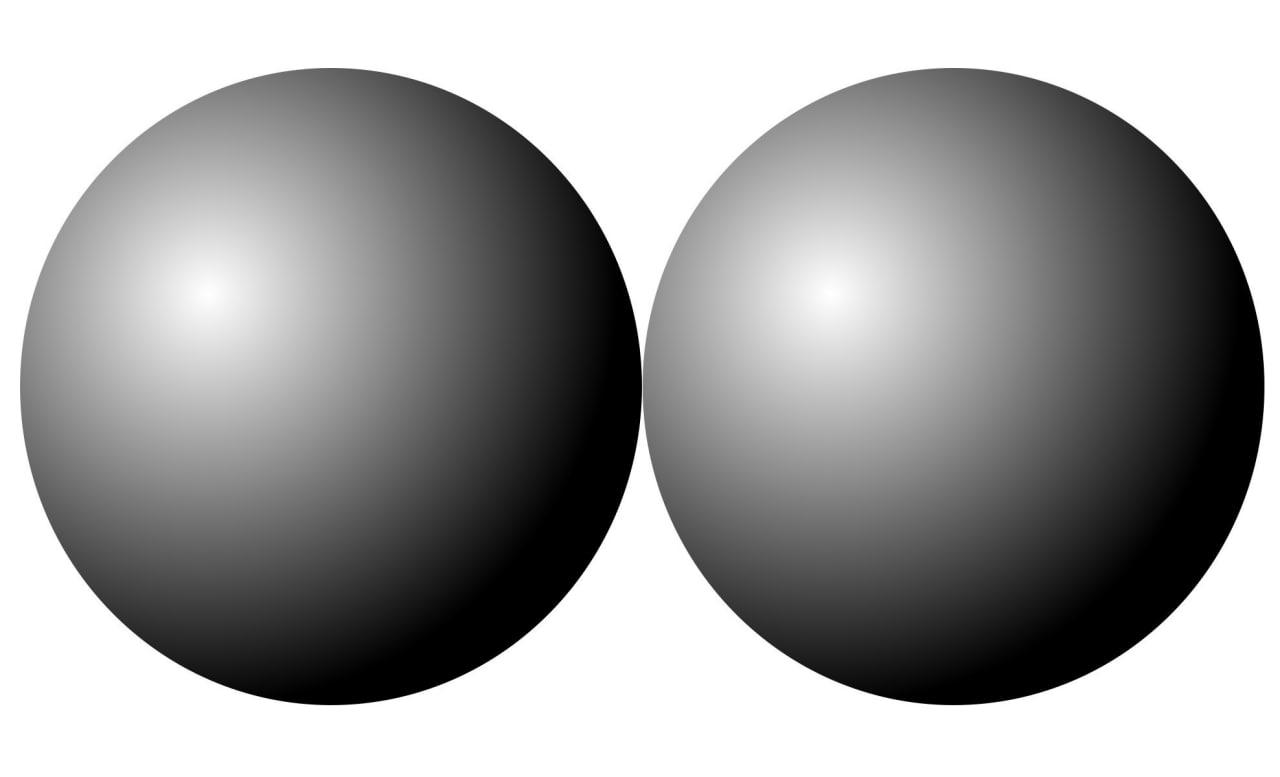
\includegraphics[width=0.33\textwidth]{figures/dumbbell_shape.png}
    \caption{Dumbbell-shaped particle -- two spheres joined together at the touchpoint.}
    \label{fig:dumbbell_shape}
\end{figure}

In Chapter \ref{chapter:theory} of this work, we study the theory required to describe the molecular dynamics close to the wall and understand the experiment of Ref. \cite{verweij2021}. Sections \ref{sec:hydrodynamics_theory} and \ref{sec:electr_theory} refer to wall-particle hydrodynamic and electrostatic interactions, respectively. Section \ref{sec:sde_theory} describes the possible approaches to solve the SDEs governing the particle's motion, especially numerically. In Section \ref{sec:verweij_theory} we look at the experiment of Ref. \cite{verweij2021} in detail, alongside the theory proposed by the authors. We discuss its limitations and possible phenomena that were missed in their interpretation of the results. Chapter \ref{chapter:methodology} describes the methodology of this work, including various numerical techniques and codes applied in the research. In Chapter \ref{chapter:results} one can find the results of this work's investigations, beginning with the computation of the particle mobility matrix values in Section \ref{sec:mobility_results}. Section \ref{sec:unbounded_results} shows the approach to the motion of particles in an unbounded fluid body, with a particular focus on describing the angular orientation. Section \ref{sec:verweij_results} shows the reconstruction of the mentioned experimental setup and comparison of the remodelled results with the ones of Ref. \cite{verweij2021}. Finally, in Section \ref{sec:developments_results} we analyse possible developments of the proposed theory and compare them with the original results. Chapter \ref{chapter:summary} is a summary of this work.

\chapter{Molecular dynamics of the dumbbells close to the wall -- theory} \label{chapter:theory}

\section{Wall-particle hydrodynamic interactions} \label{sec:hydrodynamics_theory}

\subsection{Stokes flow}

The fluid mechanics can be generally described with the famous Navier-Stokes equations. They state that an incompressible Newtonian fluid of density $\rho$ and dynamic viscosity $\eta$ can be described with
\begin{equation}
    \rho \frac{\partial\boldsymbol{v}}{\partial t} + \rho(\boldsymbol{v \cdot \nabla})\boldsymbol{v} = \eta\Delta\boldsymbol{v}-\nabla p + \boldsymbol{f},
\label{eqn:incompressible_ns}
\end{equation}
\begin{equation}
    \boldsymbol{\nabla \cdot v}=0,
\label{eqn:incompressibility_condition}
\end{equation}
where $\boldsymbol{v}=\boldsymbol{v}(\boldsymbol{r},t)$ is the fluid velocity in the point $\boldsymbol{r}$ and time $t$. The velocity field is affected by the pressure $p=p(\boldsymbol{r},t)$ and the external forces density $\boldsymbol{f}$, often simply associated with gravitational effects. Equation \eqref{eqn:incompressibility_condition} is called the incompressibility condition -- intuitively, it stands for the condition of the conservation of mass at constant fluid density.

The Navier-Stokes Equations can be rewritten in terms of the characteristic scales for the length $L_0$, time $T_0$, velocity $V_0$ and pressure $P_0=\rho V_0^2$ (as in Bernoulli's principle \cite{batchelor_2000}). For each of them, the dimensionless variables are, respectively: $\boldsymbol{x}^*=\boldsymbol{x}/L_0$, $t^*=t/T_0$, $\boldsymbol{v}^*=\boldsymbol{v}/V_0$ and $p^*=p/\rho V_0^2$. Then, Equation \eqref{eqn:incompressible_ns} can be expressed as
\begin{equation}
    \frac{\partial \boldsymbol{v}^*}{\partial t^*} 
    + \boldsymbol{v}^*\boldsymbol{\cdot\nabla}^*\boldsymbol{v}^* 
    = -\frac{1}{\rho V_0^2}\nabla^*p^* 
    + \frac{1}{Re}\nabla^{*2}\boldsymbol{v}^* 
    + \frac{L}{\rho U^2}\boldsymbol{f}^*,
\label{eqn:dimensionless_ns}
\end{equation}
where $\nabla^*=L_0\nabla$ is the dimensionless gradient operator, $\boldsymbol{f}^*$ is a dimensionless force density and $Re=\rho V_0 L_0 / \eta$ is the Reynolds number. The latter is the ratio of inertial to viscous effects in the fluid -- roughly speaking, it says whether the flow is more turbulent or laminar. For the colloidal particles, which are our main point of interest, the characteristic scales can vary as $L_0\sim0.1 - 10$ $\mu$m and $V_0\sim1 - 100$ $\mu$m/s. These very low Reynolds numbers indicate that viscous forces dominate over inertial forces in the system. Therefore, the Reynolds numbers for such systems vary in the range of $Re \sim 10^{-7}-10^{-3}$ for the viscosity and density of water \cite{klumpp_2019}. As a result, the inertial terms on the LHS of Eq. \eqref{eqn:dimensionless_ns} can be neglected. This simplification is characteristic of colloidal suspensions, where viscosity plays a key role in determining the dynamics of the particles. Setting the inertial terms to zero and multiplying by $\rho V_0^2/L_0$ one can obtain
\begin{equation}
    \eta \nabla^2 \boldsymbol{v} = \nabla p - \boldsymbol{f}
\label{eqn:stokes_equation}
\end{equation}
which, together with the incompressibility condition of Eq. \eqref{eqn:incompressibility_condition}, forms the Stokes equations.

\subsection{Mobility matrix of an axisymmetric particle} \label{sec:axisymmetric_mobility_theory}

The Stokes equations are widely used to describe small Reynolds number flows. Their main advantage is linearity, which simplifies multiple physical problems. One such problem is a particle immersed in a fluid and the relation between its velocity and force acting on it. The flow around this particle can be described by the Stokes equations and superposed with the ambient time-independent flow velocity $\boldsymbol{v}_0(\boldsymbol{r})$, vorticity $\boldsymbol{\omega}(\boldsymbol{r}) = \frac{1}{2}\nabla \times \boldsymbol{v}_0$ and strain rate $\boldsymbol{E}_0(\boldsymbol{r}) = \overbar{\nabla \boldsymbol{v}_0(\boldsymbol{r})}$, with the bar denoting the symmetric and traceless part. Due to the linearity of the Stokes equations and the boundary conditions, we can assume that force $\boldsymbol{F}$, torque $\boldsymbol{T}$ and symmetric dipole moment $\boldsymbol{S}$ acting on the particle are linearly related to the velocity, vorticity and strain rate via some specific coefficients, called the resistance coefficients. This relation can be expressed as
\begin{equation}
    \begin{pmatrix}
    \boldsymbol{F}\\\boldsymbol{T}\\\boldsymbol{S}
    \end{pmatrix}=\begin{pmatrix}
    \bm{\zeta}^{\textrm{tt}} & \bm{\zeta}^{\textrm{tr}} & \bm{\zeta}^{\textrm{td}} \\
    \bm{\zeta}^{\textrm{rt}} & \bm{\zeta}^{\textrm{rr}} & \bm{\zeta}^{\textrm{rd}} \\
    \bm{\zeta}^{\textrm{dt}} & \bm{\zeta}^{\textrm{dr}} & \bm{\zeta}^{\textrm{dd}}
    \end{pmatrix}
    \begin{pmatrix}
    \boldsymbol{v}_0(\boldsymbol{r})-\boldsymbol{V}\\
    \boldsymbol{\omega}_0(\boldsymbol{r})-\boldsymbol{\Omega}\\
    \boldsymbol{E}_0(\boldsymbol{r})
    \end{pmatrix},
\label{eqn:resistance_matrix}
\end{equation}
where $\boldsymbol{V}$ and $\boldsymbol{\Omega}$ are the particle's translational and rotational velocity, respectively. The relation between forces and velocities is governed by the resistance matrix $\left( \bm{\zeta}^{\textrm{tt}} \ldots \bm{\zeta}^{\textrm{dd}} \right)$, which describes how the particle resists the forces acting on it. Each component of this matrix explains the relation between each type of motion and stress. For example, $\bm{\zeta}^{\textrm{tt}}$ determines the relation between the linear force $\boldsymbol{F}$ and particle's translational velocity $\boldsymbol{v}$, whereas $\bm{\zeta}^{\textrm{tr}}$ describes the translation-rotation coupling between $\boldsymbol{F}$ and $\boldsymbol{\Omega}$. It is important to note that all the elements of forces and velocities vectors contain three components, and each element of the resistance matrix has the dimension of $3\times 3$.

In many cases, you can restrict your attention to the force and torque, and therefore the resistance matrix can be reduced to its upper left minor. Also, one can define the mobility matrix $\bm{\mu}$, which for the strainless variant of $\bm{\zeta}$ is
\begin{equation}
    \bm{\mu}=\begin{pmatrix}
    \bm{\mu}^{\textrm{tt}} & \bm{\mu}^{\textrm{tr}}\\
    \bm{\mu}^{\textrm{rt}} & \bm{\mu}^{\textrm{rr}}
    \end{pmatrix}=\begin{pmatrix}
    \bm{\zeta}^{\textrm{tt}} & \bm{\zeta}^{\textrm{tr}}\\
    \bm{\zeta}^{\textrm{rt}} & \bm{\zeta}^{\textrm{rr}}\\
    \end{pmatrix}^{-1}=\bm{\zeta}^{-1}.
\label{eqn:mobility_matrix}
\end{equation}

The mobility matrix $\bm{\mu}$ is exactly the inverse of the resistance matrix $\bm{\zeta}$. In fact, it answers the reverse question: \textit{What will be the particle's velocities if we know the forces acting on it?} Indeed, this is what we usually seek in the particle dynamics simulations -- knowing the estimated forces, we calculate the velocities to determine the particle position and orientation in each time step.

For an axisymmetric particle in the vicinity of a wall, the mobility matrix obeys multiple symmetries and many of the mobility matrix components of $\bm{\mu}^{ij}$ are equal to zero, as derived by Lisicki \textit{et al.} \cite{lisicki2016}. The cartesian components of specific mobility coefficients depend on the particle's position and orientation. The Cartesian position can be described with the distance between the wall and the particle's centre of mass $h_{\textrm{c.m.}}$, whereas the orientation is described with $\theta$ -- the angle between the particle's symmetry axis and any wall-parallel plane. To make the description clearer, it is useful to introduce a parameter $w=\cos\theta$, as well as a particle-fixed frame of reference RW (rod-wall). This frame is defined by three unit vectors ($\hat{\boldsymbol{u}}_1$,$\hat{\boldsymbol{u}}_2$,$\hat{\boldsymbol{u}}_3$), where $\hat{\boldsymbol{u}}_1$ is pointing along the particle's axis of symmetry. The other two components are defined as
\begin{equation}
    \hat{\boldsymbol{u}}_2=\frac{\hat{\boldsymbol{e}}_z\times\hat{\boldsymbol{u}}_1}{|\hat{\boldsymbol{e}}_z\times\hat{\boldsymbol{u}}_1|} \hspace{.6cm} \hat{\boldsymbol{u}}_3=\hat{\boldsymbol{u}}_2\times\hat{\boldsymbol{u}}_1,
\label{eqn:wr_frame}
\end{equation}
where $\hat{\boldsymbol{e}}_z$ is the wall-normal unit vector, pointing upwards. Fig. \ref{fig:wr_frame} shows a schematic illustration of the particle-fixed RW frame.
\begin{figure}
    \centering
    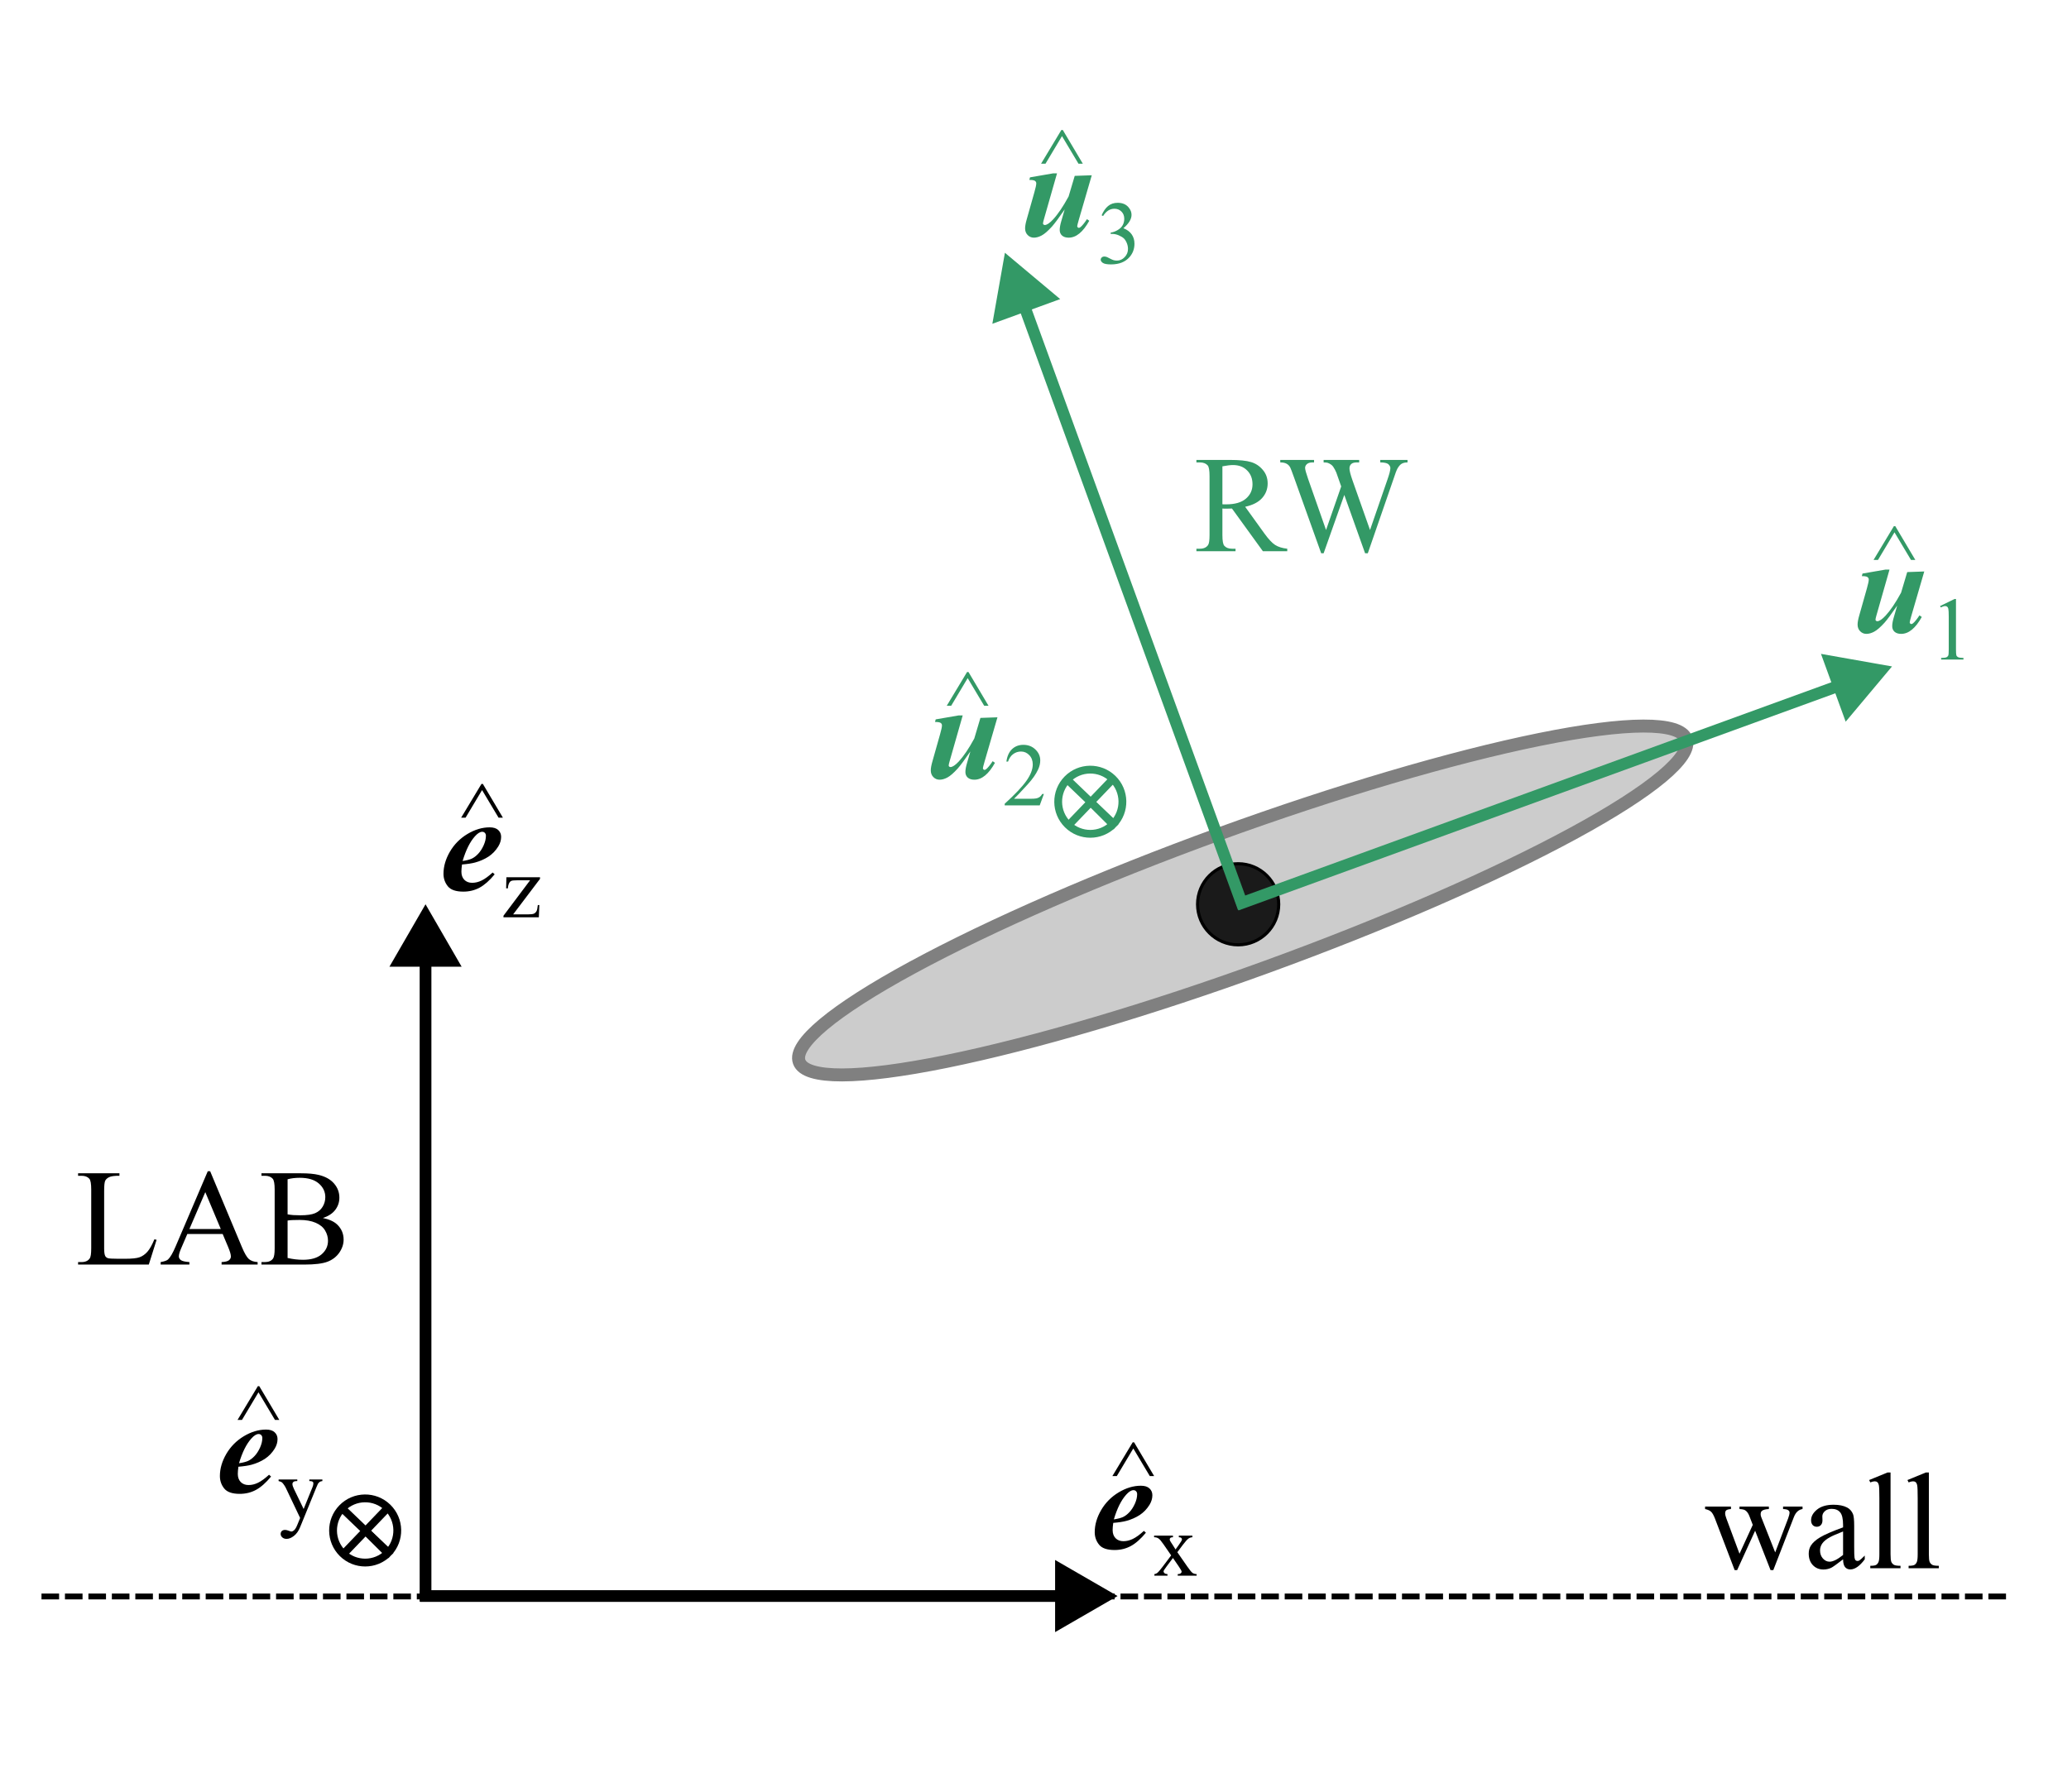
\includegraphics[width=0.43\linewidth]{figures/rw_frame.png}
    \caption{Schematic illustration of the particle-fixed RW frame. Unit vector $\hat{\boldsymbol{u}}_1$ is pointing along the particle's symmetry axis, whereas $\hat{\boldsymbol{u}}_2$ and $\hat{\boldsymbol{u}}_3$ are normal to the axis. The unit vector $\hat{\boldsymbol{u}}_2$ is defined as always parallel to the wall.}
    \label{fig:wr_frame}
\end{figure}
In these selected coordinates, the components of the translational mobility matrix become
\begin{equation}
    \bm{\mu}^{\textrm{tt}}(h,w)=\begin{pmatrix}
    a_{\textrm{t}}(h,w) & 0 & c_{\textrm{t}}(h,w) \\
    0 & b_{\textrm{t}}(h,w) & 0 \\
    c_{\textrm{t}}(h,w) & 0 & d_{\textrm{t}}(h,w)
    \end{pmatrix}_{\textrm{RW}}.
\label{eqn:mobility_tt}
\end{equation}

Most of the symmetries of $\bm{\mu}^{\textrm{tt}}$ hold due to the vector $\hat{\boldsymbol{u}}_2$ being normal to the particle's symmetry axis and always parallel to the wall. Therefore, the velocity or force in the direction normal to $\hat{\boldsymbol{u}}_2$ (superposition of $\hat{\boldsymbol{u}}_1$ and $\hat{\boldsymbol{u}}_3$) does not induce any translational coupling. The rotational mobility matrix has an analogous structure as the translational one.

When it comes to the translation-rotation coupling, the mobility matrix structure is different, defined as
\begin{equation}
    \bm{\mu}^{\textrm{tr}}(h,w)=\begin{pmatrix}
    0 & a_{\textrm{tr}}(h,w) & 0 \\
    b_{\textrm{tr}}(h,w) & 0 & c_{\textrm{tr}}(h,w) \\
    0 & d_{\textrm{tr}}(h,w) & 0
    \end{pmatrix}_{\textrm{RW}},
\label{eqn:mobility_tr}
\end{equation}
for which the exactly opposite elements of the matrix vanish. For example, a force pointing along $\hat{\boldsymbol{u}}_1$ does not induce rotation around the symmetry axis of the particle. However, the induced rotation around $\hat{\boldsymbol{u}}_2$ is possible and described with $a_{\textrm{tr}}(h,w)$. Looking at an example depicted in Fig. \ref{fig:wr_frame}, we see that one of the rod's ends can interact with the wall differently than the other due to different distances between them and a boundary. Therefore, both of the parameters $h$ and $w$ are crucial to determine the particle's configuration with respect to the wall and the mobility coefficients.

Even though the matrices' structures seem quite simplified, finding the analytical expressions for the individual mobility components is difficult. The work of Lisicki \textit{et al.} \cite{lisicki2016} provides analytical approximations of the resistance matrix and its dependencies on ($h$,$w$). Each element of $\bm{\zeta}$ is approximated by a polynomial of given elements of the particle's resistance matrix $\bm{\zeta}_0$ infinitely far from the wall, trigonometric functions of the orientation $\sin\theta$ and $\cos\theta$, and particle-wall separation $h$ (see Eq. 12-20 in Ref. \cite{lisicki2016}). However, these equations are simply expansions with respect to $h^{-1}$ and they do not consider the lubrication effects, which are significant when the gap height $h_{\textrm{g}}$ between the particle surface and wall becomes much smaller than the particle size. Luckily, we can find these solutions numerically with very good accuracy, provided by the \code{HYDROMULTIPOLE} code \cite{cichocki2000}, described in Section \ref{sec:methodology:hydromultipole}. Nonetheless, to understand the code's methodology, one should first familiarise oneself with the concept of Blake's tensor, described below.

\subsection{Blake's tensor and its extensions}

To better understand the relation between velocity and force acting on a colloidal particle, let us imagine a single point force with density $\boldsymbol{f} = \bm{\delta}(\boldsymbol{r} - \boldsymbol{r}_0) \boldsymbol{F}$, applied at the point $\boldsymbol{r}_0$ in a fluid body. Such entity is called a Stokeslet, and its magnitude is $F=|\boldsymbol{F}|$. The resultant fluid velocity field $\boldsymbol{v}$ in the point $\boldsymbol{r}$ can be described as
\begin{equation}
    \boldsymbol{v}(\boldsymbol{r}) = \mathsfbi{T}_0(\boldsymbol{r} - \boldsymbol{r}_0) \cdot \boldsymbol{F},
\label{eqn:stokeslet_velocity}
\end{equation}
where $\mathsfbi{T}_0(\boldsymbol{r}) = (\hat{\bm{1}} + \hat{\boldsymbol{r}}\hat{\boldsymbol{r}}) / 8 \pi \eta r$ is called the Oseen tensor \cite{kim_karilla}, $r = |\boldsymbol{r}|$ and $\hat{\boldsymbol{r}}=\boldsymbol{r}/r$. A flow induced by the Stokeslet is presented in Fig. \ref{fig:stokeslets}a. The streamlines are predominantly aligned with force direction, with characteristic narrowing in behind and expansion before the Stokeslet. The flow is symmetrical with respect to the force's axis due to the system's lack of any boundaries.

\begin{figure}
    \centering
    \includegraphics[width=\linewidth]{figures/stokeslets.png}
    \caption{ \textbf{a)} Streamlines of a Stokeslet-induced flow in an infinite fluid body. \textbf{b)} Streamlines of a Stokeslet placed in the vicinity of a wall, pointing parallel to the wall's plane. The wall is symbolised with a thicker line at the bottom. \textbf{c)} An analogous to b), with the force directed normal to the boundary. The plots a)-c) were reproduced from Ref. \cite{lisicki_nagele_2016} (Fig. 7a and 18). \textbf{d)} Blake's original illustrations of the wall's screening of a wall-parallel Stokeslet, placed at the separation $h$ above the boundary. An image system is constructed from the three multipole solutions, pointing in specific directions. \textbf{e)} Blake's multipole solution for the wall-normal Stokeslet.}
    \label{fig:stokeslets}
\end{figure}

In case of homogenous boundary conditions standard result from Green's function theory applies, where
\begin{equation}
    \boldsymbol{v}(\boldsymbol{r}) = \boldsymbol{v}_0(\boldsymbol{r}) + \int d\boldsymbol{r}' \mathsfbi{T}(\boldsymbol{r}, \boldsymbol{r}') \cdot \boldsymbol{f},
\end{equation}
with $\mathsfbi{T}(\boldsymbol{r}, \boldsymbol{r}')$ being the Green's function \cite{lisicki_2013}. The above equation can also be solved for the case of a Stokeslet placed above the impenetrable wall at a distance $h$, with the no-slip boundary condition $\boldsymbol{v}=0$ at the interface. Such a solution has been found by Lorentz \cite{lorentz_1907}. Thanks to the linearity of the equations, we can use the method of images to describe the flow. The Green's function would be then given as $\mathsfbi{T}(\boldsymbol{r}, \boldsymbol{r}') = \mathsfbi{T}_0(\boldsymbol{r} - \boldsymbol{r}_0) + \mathsfbi{T}_\textrm{w}(\boldsymbol{r}, \boldsymbol{r}')$, where the latter is the wall-screened term, often referred as the Blake's tensor, given by
\begin{equation}
    \mathsfbi{T}_\textrm{w}(\boldsymbol{r}, \boldsymbol{r}') = -\mathsfbi{T}_0(\boldsymbol{r} - \boldsymbol{r}'^*) \cdot \mathsfbi{P} - 2h\hat{\bm{e}}_z \cdot \mathsfbi{T}_0(\boldsymbol{r} - \boldsymbol{r}'^*) \overleftarrow{\nabla}_{\boldsymbol{r}} \cdot \mathsfbi{P} + h^2 \nabla_{\boldsymbol{r}}^2 \mathsfbi{T}_0(\boldsymbol{r} - \boldsymbol{r}'^*) \cdot \mathsfbi{P},
\label{eqn:blakes_tensor}
\end{equation}
where $[\hat{\bm{a}}\overleftarrow{\nabla}_{\boldsymbol{r}}]_{\alpha\beta}=\partial a_\alpha / \partial r_\beta$ and $\mathsfbi{P}$ is the reflection operator, mirroring any point with respect to the wall's plane. The consecutive terms in the RHS of Eq. \eqref{eqn:blakes_tensor} are the zeroth, first and second derivative of the Oseen tensor. In the work of Blake \cite{blake1971}, they are interpreted as the subsequent multipole solutions: the Stokeslet, the Stokes doublet and the Source doublet, all placed in $\boldsymbol{r}'^*$. The Stokes doublet can be interpreted as the flow induced by two Stokeslets pointing in opposite directions, separated by an infinitely small distance. Its magnitude is equal to $-2hF$ or $2hF$ for the original Stokeslet directed normal and parallel to the wall, respectively. The Source consists of two Stokes doublets separated by $h$, and its magnitude varies from $-2h^2F$ to $2h^2F$.

The complete superpositions are presented in Fig. \ref{fig:stokeslets}, which consist of the original illustrations from Blake's work \cite{blake1971} for the Stokeslet oriented parallel (d) and normal (e) to the wall. For both cases, the image Stokeslets are parallel to the original ones but have opposite directions. The Stokes doublet consists of two Stokeslets pointing in the two wall-normal directions in two possible configurations as depicted in Fig. \ref{fig:stokeslets}. Then, the Source doublets can also be placed on the axis, either normal or parallel to the wall. The resultant flows are also presented in Fig. \ref{fig:stokeslets}. While the unbounded fluid flow (a) is symmetrical with respect to the axis direction, the wall's presence significantly affects the velocity field. When the Stokeslet is wall-parallel (b), the streamlines resemble the unbounded ones but are slightly pushed away by the wall. The tangent force streamline especially shows how the wall repels the Stokeslet. However, the flow becomes significantly different for the wall-normal configuration (c). In this case, the fluid is pushed more strongly in the force direction, and the suction between the Stokeslet and the wall is more pronounced. For forces in directions other than parallel or normal, the flow is simply a superposition of these two configurations (due to the linearity of the Stokes equations).

The point force concept is useful for investigating systems where the particle's size is negligible compared to the separation from the wall. However, in the case of non-negligible particle sizes, we need first to find the force density $\boldsymbol{f}(\boldsymbol{r})$, which then would allow us to calculate the overall force $\boldsymbol{F}=-\int_\Sigma\boldsymbol{f}(\boldsymbol{r})d\boldsymbol{r}$ via integration over the particle's surface $\Sigma$. An approach comprehensively described by Ekiel-Jeżewska and Wajnryb \cite{ekiel_2009} is a convenient way to approximate the force density $\boldsymbol{f}(\boldsymbol{r})$ and the velocity field $\boldsymbol{v}(\boldsymbol{r})$. This method is based on expressing these two quantities on the surface of the conglomerate of $N$ spherical particles in the form of a boundary integral equation projected onto a complete set of multipolar solutions of the Stokes equations. Due to the induced forces concept \cite{albano_1975}, we can extend our Stokes flow calculations inside the spherical particles. Then, in an ambient flow of velocity $\boldsymbol{v}_0(\boldsymbol{r})$, the velocity field $\boldsymbol{v}_i(\boldsymbol{r})$ on the surface of particle $i$ can be expressed as
\begin{equation}
    \boldsymbol{v}_i(\boldsymbol{r}) = \sum_{j=1}^N \mathsfbi{T}_0(\boldsymbol{r} - \boldsymbol{r}_0) \cdot \boldsymbol{f}_j(\boldsymbol{r}'),
\label{eqn:stokeslet_velocity2}
\end{equation}
where $\boldsymbol{f}_j(\boldsymbol{r}')$ is the force density on the $j$-particle's surface. The self-contribution term $i=j$ can be expressed as $\boldsymbol{f}_i=-\boldsymbol{Z}_{0,i}(\boldsymbol{v}_i - \boldsymbol{v}_0)$, where $\boldsymbol{Z}_{0,i}$ is the single-particle resistance operator. For the sphere-sphere contribution ($i\neq j$), we can define the Green's function $\boldsymbol{G}_{ij}$ as
\begin{equation}
    [\boldsymbol{G}_{ij}\boldsymbol{f}_j](\boldsymbol{r}) = \int d\boldsymbol{r}' \mathsfbi{T}(\boldsymbol{r},\boldsymbol{r}') \cdot \boldsymbol{f}_j(\boldsymbol{r}'),
\end{equation}
where $\boldsymbol{r}$ belongs to the surface of the particle $i$. Then, we can write that
\begin{equation}
    \boldsymbol{v}_i - \boldsymbol{v}_0 = \boldsymbol{Z}_{0,i}^{-1} \boldsymbol{f}_i + \sum_{j \neq i}^{N} \boldsymbol{G}_{ij} \boldsymbol{f}_j,
\end{equation}
where $i=1, \cdots, N$. The velocity field and force densities in the equations above can be expanded into multipoles, analogous to the ones of Blake \cite{blake1971}. Then, they can be truncated at a given multipole order, for example, $L=4$ (Stokes-doublet is of order $L=1$, Source-doublet is $L=2$). Then, we can numerically solve a set of linear equations, where we put all the velocities $\boldsymbol{v}_i - \boldsymbol{v}_0$ into a vector $\boldsymbol{c}$ and we arrange all the force multipole moments $\boldsymbol{f}_i$ into a vector $\boldsymbol{f}$. Then, $\mathsfbi{Z}_{0}^{-1}$ and $\mathsfbi{G}$ become matrices and
\begin{equation}
    \boldsymbol{c} = \left( \mathsfbi{Z}_0^{-1} + \mathsfbi{G} \right) \cdot \boldsymbol{f},
\end{equation}
which resembles Eq. \eqref{eqn:resistance_matrix} for the resistance matrix $\bm{\mu}$. Indeed, the reverse problem is
\begin{equation}
    \boldsymbol{f} = \mathsfbi{Z} \cdot \boldsymbol{c},
\end{equation}
where $\mathsfbi{Z}$ is the friction matrix. We can find it numerically by solving the abovementioned linear equations for the multipoles of a given order. Then, after calcutating the wall-screening corrections (see Ref. \cite{ekiel_2009} or Appendix B of Ref. \cite{lisicki2016}) to the friction matrix $\mathsfbi{Z}$, we finally obtain the resistance matrix $\bm{\zeta}$.

The methodology briefly explained above is employed in the \code{HYDROMULTIPOLE} code, discussed in more detail in Section \ref{sec:methodology:hydromultipole}. This algorithm is used in the numerical findings of the dumbbell particle's mobility matrix, presented in Section \ref{sec:mobility_results}. However, let's first focus on another crucial topic of the research presented in this thesis, namely the stochastic differential equations.

\section{The stochastic differential equations of particle motion} \label{sec:sde_theory}

\subsection{Langevin and Itō approach}

In the description of colloidal particle dynamics, a crucial topic is the influence of Brownian motion, which was first observed by Brown in 1828 \cite{brown_1828} and later explained by Einstein \cite{einstein1905,einstein1906} and Smoluchowski \cite{smoluchowski1906} in 1905 and 1906. The Brownian particle, which in this thesis can be understood as an equivalent of the colloidal particle, experiences an enormous number of collisions each second with fluid particles surrounding it. For a colloidal particle of a diameter $d \sim1 \textrm{ }\mu\textrm{m}$ suspended in water, the collision rate is $\sim 10^{19}$ s$^{-1}$. Due to the fluctuations of this collision rate, the particle experiences a random force that is modelled as normally distributed. The difficulty in the description of this force is its vanishingly small correlation time, scaling as the speed of sound in the given fluid and the particle size, meaning that $\textrm{E}[\boldsymbol{F}_n(t)\boldsymbol{F}_n(t')]=0$ for two different values of time $t \neq t'$, where $\textrm{E}[x]$ is an expected value of the variable $x$. There were various approaches to cope with Brownian motion randomness, developed by Smoluchowski \cite{smoluchowski1906}, Fokker \cite{fokker1914} and Planck \cite{planck1917} or Langevin \cite{langevin1908}. The latter proposes to describe the particle's position $\boldsymbol{x}$ as
\begin{equation}
    m \ddot{\boldsymbol{x}} = -\zeta \dot{\boldsymbol{x}} + \boldsymbol{F}(\boldsymbol{x},t) + \boldsymbol{F}_n(t),
\label{eqn:langevin}
\end{equation}
where $\dot{\boldsymbol{x}}$ and $\ddot{\boldsymbol{x}}$ are the first and second time derivatives of $\boldsymbol{x}$. The coefficient $\zeta$ is the measure of the resistance of the fluid in which the particle is immersed and for now we assume it does not depend on $\boldsymbol{x}$ (see Eq. \eqref{eqn:translational_timestep}). Besides the noise term $\boldsymbol{F}_n(t)$, there is also an arbitrary external force $\boldsymbol{F}(\boldsymbol{x},t)$. What is more to say about $\boldsymbol{F}_n(t)$ is that its covariance at given temperature $T$ is equal to $E [ \boldsymbol{F}_n(t)\boldsymbol{F}_n(t') ] =  2 k_B T \zeta \delta(t-t') $, where $k_B$ is the Boltzmann constant.

Although the Langevin formalism is a standard tool used to describe the Brownian motion, solving this equation remains difficult, since the force $\boldsymbol{F}_n(t)$ still remains unpredictable. The variation of $\boldsymbol{F}_n(t)$ over any given time interval is infinite and therefore, it is impossible to calculate the Lebesgue integral. The correct mathematical formalism to address the issue of non-integrability in the Lebesgue sense of the fluctuating force is to express the motion in terms of a Stochastic Differential Equation (SDE) form, that captures both deterministic and stochastic components in a well-posed manner. To mimic the Langevin formalism, SDEs are often written in terms of the infinitesimals as a change $\boldsymbol{dx}$ of position $\boldsymbol{x}(t)$ in time $t$ and after a time step $dt$, written as
\begin{equation}
    \boldsymbol{dx}(t+dt) = \boldsymbol{a}(\boldsymbol{x}(t),t)dt + \boldsymbol{b}(\boldsymbol{x}(t),t)\boldsymbol{dW}(t),
\label{eqn:sde_general}
\end{equation}
where $\boldsymbol{a}(\boldsymbol{x}(t),t)$ is called the drift term, fully deterministic and fluctuation-free, and the element $\boldsymbol{b}(\boldsymbol{x}(t),t)$ is the diffusion (or noise) term that characterises the stochastic part of the equation, especially its strength. It is multiplied by $\boldsymbol{dW}(t)$, which is the Wiener process that captures the stochastic nature of Brownian motion. It is defined as the unique Gaussian martingale process with mean $\textrm{E}[\boldsymbol{dW}(t)]=0$ and covariance $\textrm{E}[\boldsymbol{dW}(t_1)\boldsymbol{dW}(t_2)] = \textrm{min}(t_1, t_2)$. An approach coherent with Eq. \eqref{eqn:sde_general} was developed by Itō \cite{ito1951} and is given as
\begin{equation}
    \boldsymbol{dx} = \bm{\mu} \boldsymbol{F} dt + \sqrt{2 D} \boldsymbol{dW},
\label{eqn:ito}
\end{equation}
where $\bm{\mu}\boldsymbol{F} dt$ is the drift term and $\boldsymbol{F}$ is simply the external force acting on a particle. The noise term is given by the diffusion coefficient $D$ and the Wiener process $\boldsymbol{dW}$, for which we omit the time-dependence.  Eq. \eqref{eqn:ito} is convenient for the simulations due to the similarities with the commonly used Euler-Maruyama  approach that can be derived via Taylor-Itō expansion (see Section \ref{sec:methodology_pychastic}). It calculates the particle displacement $\boldsymbol{dx}$ for each time step $dt$. The Wiener process is easy to obtain in each step as well. The Eq. \eqref{eqn:sde_general} and \eqref{eqn:ito} should be understood in a weak (distributional) sense with respect to the Itō integral, that is
\begin{equation}
    \boldsymbol{x}(\tau) = \int_0^{\tau}\boldsymbol{dx}=\int_0^{\tau} F(\boldsymbol{x},t) + \int_0^{\tau}\sqrt{2D}\boldsymbol{dW},
\label{eqn:ito_integral}
\end{equation}
where all the integrals of Eq. \eqref{eqn:ito_integral} are taken in Itō sense. This approach allows one to create an equation to simulate a change $\boldsymbol{dx}$ of the chosen particle's position $\boldsymbol{x}(t)$ in time $t$ after a timestep $dt$. It is given as
\begin{equation}
    \boldsymbol{dx} = k_BT\frac{\partial\bm{\mu}(\boldsymbol{x})}{\partial \boldsymbol{x}} dt + \sqrt{2 k_B T} \boldsymbol{dW}.
\label{eqn:translational_timestep}
\end{equation}
Here, we assume that the mobility matrix may depend on the particle's position $\boldsymbol{x}$, for example due to the presence of a confinement in the system. The gradient of the mobility matrix $\partial \bm{\mu}(\boldsymbol{x}) / \partial \boldsymbol{x}$ determines the drift. The last term introduces the Brownian effects (noise) to the system. To solve the Eq. \eqref{eqn:translational_timestep} in a satisfactory time and stay in the user-friendly environment of Python, we can use the \code{pychastic} package \cite{waszkiewicz2023}, described in detail in Section \ref{sec:methodology_pychastic}. Roughly speaking, it uses the Itō formalism to solve the SDEs given by the user in an analogous form to Eq. \eqref{eqn:ito} -- split into the drift and noise term. With this powerful tool it is possible to simulate not only the translational movement of a particle but its rotation as well.

\subsection{Description of the particle orientation} \label{sec:evensen_theory}

A description of the particle's translational movement in Cartesian coordinates is a simple task using Eq. \eqref{eqn:ito}. However, simulations of the angular orientation are more complex. Usually, the orientation is described with Euler angles, which define three consecutive rotations of the coordinate system about the specific axes. However, the equations of motion in these coordinates contain strong singularities around the polar orientations. These singularities lead to numerical instabilities and undefined behaviour when the particle approaches certain orientations. Therefore, there is a need to apply a different approach, presented in the work of Evensen \textit{et al.} \cite{evensen2008}. Its main idea emerges from the Euler's rotation theorem, which says that every change of angular position can be described as the rotation by an angle $\Phi$ around a specific unit rotation vector $\bm{\delta}$. Then, the generalised coordinates are the Cartesian components $a_1$, $a_2$, $a_3$ of the rotation vector $\boldsymbol{q} = \Phi \bm{\delta} = \left( a_1, a_2, a_3 \right)$. A change $\boldsymbol{dq}$ of the particle's angular orientation $\boldsymbol{q}(t)$ in time $t$, for each timestep $dt$, can be described as
\begin{equation}
    \boldsymbol{dq} = \left[\bm{\mu}(\boldsymbol{q})\cdot \boldsymbol{F}^{\textrm{(m)}} + k_BT \frac{\partial}{\partial\boldsymbol{q}}\cdot\bm{\mu}(\boldsymbol{q}) \right] dt    +\sqrt{2k_BT}\textrm{ }\bm{\Xi}\cdot\bm{\Omega}^\textrm{T}\cdot\bm{\mu}^{(\omega)}_{\textrm{d}}\cdot\boldsymbol{dW},
\label{eqn:rotational_timestep}
\end{equation}
where the second term emerges from the choice of specific coordinate system and it ensures that the equilibrium distribution equals the Boltzmann distribution. Usually $\boldsymbol{F}^{\textrm{(m)}}$ is called a metric force and it is defined as
\begin{equation}
    \boldsymbol{F}^{\textrm{(m)}}=k_BT\left(\frac{\textrm{sin}\Phi}{1-\textrm{cos}\Phi}-\frac{2}{\Phi}\right)\bm{\delta}^{(a)}.
\label{eqn:metric_force}
\end{equation}

In the Eq. \eqref{eqn:rotational_timestep} the mobility matrix $\bm{\mu}$ is expressed in the LAB frame of reference. Its gradient with respect to $\boldsymbol{q}$ is taken into account in the third term and it ensures that the particle tends to the lowest potential configuration. Let's write the particle-fixed mobility matrix as $\bm{\mu}^{(\omega)}$. Since the Cartesian particle-fixed coordinate system coincides with the principal axes of the mobility matrix, $\bm{\mu}^{(\omega)}$ is always diagonal. The last part of the Eq. \eqref{eqn:rotational_timestep} accounts for the stochastic term, for which we need a root of the particle-fixed mobility matrix $\bm{\mu}^{(\omega)}_{\textrm{d}}$, described as
\begin{equation}
    \bm{\mu}^{(\omega)}_{\textrm{d}}=
    \begin{pmatrix}
    \sqrt{\mu^{(\omega)}_1} & 0 & 0\\
    0 & \sqrt{\mu^{(\omega)}_2} & 0\\
    0 & 0 & \sqrt{\mu^{(\omega)}_3}
    \end{pmatrix}.
\end{equation}

The matrices $\tilde{\bm{\Omega}}$ and $\tilde{\bm{\Xi}}$ from the Eq. \eqref{eqn:rotational_timestep} are the rotation and transformation matrix, respectively. The first one rotates the mobility matrix from the particle-fixed frame to the wall-fixed one. The second matrix transforms the coordinates to the Cartesian components of $\boldsymbol{q}$. In terms of $(a_1,a_2,a_3)$ and $\Phi$ they are expressed as
\begin{equation}
    \begin{split}
    \bm{\Omega}=\frac{1}{\Phi^2}
    \begin{pmatrix}
    \Phi^2\textrm{cos}\Phi & -a_3\Phi\textrm{sin}\Phi & a_2\Phi\textrm{sin}\Phi\\
    a_3\Phi\textrm{sin}\Phi & \Phi^2\textrm{cos}\Phi & -a_1\Phi\textrm{sin}\Phi\\
    -a_2\Phi\textrm{sin}\Phi & a_1\Phi\textrm{sin}\Phi & \Phi^2\textrm{cos}\Phi
    \end{pmatrix}\\
    +\frac{1-\textrm{cos}\Phi}{\Phi^2}
    \begin{pmatrix}
    a_1a_1 & a_1a_2 & a_1a_3\\
    a_2a_1 & a_2a_2 & a_2a_3\\
    a_3a_1 & a_3a_2 & a_3a_3
    \end{pmatrix},
    \end{split}
\label{eqn:omega}
\end{equation}
\begin{equation}
    \begin{split}
    \bm{\Xi}=\left(\frac{1}{\Phi^2}-\frac{\textrm{sin}\Phi}{2\Phi(1-\textrm{cos}\Phi)}\right)
    \begin{pmatrix}
    a_1a_1 & a_1a_2 & a_1a_3\\
    a_2a_1 & a_2a_2 & a_2a_3\\
    a_3a_1 & a_3a_2 & a_3a_3
    \end{pmatrix}\\
    +\frac{1}{2}
    \begin{pmatrix}
    \frac{\Phi\textrm{sin}\Phi}{1-\textrm{cos}\Phi} & -a_3 & a_2\\
    a_3 & \frac{\Phi\textrm{sin}\Phi}{1-\textrm{cos}\Phi} & -a_1\\
    -a_2 & a_1 & \frac{\Phi\textrm{sin}\Phi}{1-\textrm{cos}\Phi}
    \end{pmatrix}.
    \end{split}
\label{eqn:xi}
\end{equation}

Given the equations above, angular orientation simulations become much easier to perform. However, some of the expressions can give rise to a numerical division by zero. Even though analytically they cancel out, due to the floating point arithmetic, it is helpful to introduce Taylor expansion of chosen terms in the region of $\Phi \simeq 0$. By employing this alternative formulation using generalized rotation vectors and the mobility matrix, we avoid the numerical pitfalls associated with Euler angles, ensuring accurate and stable simulations of angular motion, even near critical orientations. Moreover, the domain of rotational motion is $SO(3)$, meaning that the coordinates $\boldsymbol{a} = (a_1, a_2, a_3)$ is limited to $|\boldsymbol{a}|\in[0,\pi\rangle$ and the rotational position values need a check of domain after each simulation step. Luckily, our algorithms can be adjusted to this easily (see Section \ref{sec:methodology_pychastic}).

\section{Wall's and particle's EDLs electrostatic interactions} \label{sec:electr_theory}

In colloidal solutions physics, electrostatic interactions play a crucial role in understanding the topic of particle-particle and particle-wall interactions. The commonly used approach is the DLVO theory, which was developed by Derjaguin and Landau in 1941 \cite{derjaguin_landau_1941}, and independently by Verweij and Overbeek in 1948 \cite{verwey_overbeek_1948}. The two primary forces in the colloidal systems are the van der Waals attraction and electrostatic interactions. The overall DLVO potential $\Psi_{\textrm{DLVO}}$ is given as
\begin{equation}
    \Psi_{\textrm{DLVO}} = \Psi_{\textrm{LJ}} + \Psi_{\textrm{el}},
\end{equation}
where $\Psi_{\textrm{LJ}}$ is the Lennard-Jones potential, chosen to represent the van der Waals attraction, and $\Psi_{\textrm{el}}$ is the electrostatic repulsion of the electric double layer. An equilibrium between these two effects provides stability in the colloidal systems. Both of the forces are described below.

\subsection{Van der Waals attraction}

The first one of the forces, van der Waals attraction, is weak and short-range interaction happening due to transient dipoles formed by fluctuations in the electron clouds of nearby atoms or molecules. A potential of these forces is often described with the Lennard-Jones potential, which for two spherical particles separated by the distance $r$ is given as
\begin{equation}
    \Psi_{\textrm{LJ}} = 4\epsilon \left( \left(\frac{\sigma}{r}\right)^{12} - \left(\frac{\sigma}{r}\right)^6 \right),
\label{eqn:lennard_jones}
\end{equation}
where $\epsilon$ determines the attraction strength and is called the depth of a potential well. Moreover, $\sigma$ is a characteristic length scale, at which $\Psi_{\textrm{LJ}}=0$. The van der Waals attraction typically operates over short distances, usually below a few nanometers, and its strength rapidly decreases with increasing separation. In contrast, electrostatic interactions, which are the primary focus of my work, dominate at larger length scales. This contrast highlights the importance of the electric repulsion for stabilizing colloidal systems over longer distances.


\subsection{Electric Double Layer}

The second one of the DLVO's forces is our main point of interest -- it is the electrostatic repulsion of the clouds of electric charge that form near the colloidal particles' surfaces. Every surface that is in contact with a fluid can become charged due to various physicochemical processes, like ionisation of surface functional groups, adsorption of ions from the solution or ion exchange with the liquid. The surface can get either a positive or negative charge, attracting the fluid's counterions. This is a mechanism of formation of a Stern layer -- a region occupied with charges of only opposite sign to the surface that are so strongly bonded to the body that they are practically immobilised. The size of the Stern layer is usually of the order of a few nanometers, similar to the length scales of van der Waals attraction.

Nonetheless, the formation of a charged layer in a fluid body causes another screening above the surface of the Stern layer. The diffuse layer consists of more loosely attracted charges of both signs, with a net value remaining the same sign as the Stern layer. This whole connected system is called an Electric Double Layer (EDL), presented in the schematic illustration of Fig. \ref{fig:double_layer}.

\begin{figure}[ht]
    \centering
    \includegraphics[width=0.65\linewidth]{figures/double_layer_fixed.png}
    \caption{Schematic illustration of the Electric Double Layer around the spherical, negatively charged particle. The characteristic regions are the particle body, the Stern layer consisting of opposite-charge particles only and the mixed-charge diffuse layer. The characteristic planes are: the particle's surface, Stern plane and slipping plane, with the values of electric potential equal to $\Psi_{\sigma}$, $\Psi_{\textrm{S}}$ and $\Psi_\zeta$, respectively. Attribution: Park \& Seo \cite{park_2011}.}
    \label{fig:double_layer}
\end{figure}

The charge density $\rho(d)$ at the distance $d$ from the charged surface can be related to the electric potential $\Psi_{\textrm{el}}$ in the fluid body via the following Poisson equation \cite{andelman_2006}, defined as
\begin{equation}
\nabla^2 \Psi_{\textrm{el}}(d) = -\rho(d)/\varepsilon,
\label{eqn:poisson}
\end{equation}
where $\varepsilon$ is the electric permittivity of the medium. At the same time, the thermal motion of ions can be described by the Boltzmann equation \cite{wikipedia_pb}. It defines the local ion density $c_i$ of each ion specie $i$ as
\begin{equation}
    c_i = c_i^0 \textrm{exp}\left( \frac{-W_i}{k_{\textrm{B}}T} \right),
\label{eqn:boltzmann}
\end{equation}
where $c_i^0$ is the ion concentration at the bulk and $W_i$ is the work needed to bring the ion from the infinite distance. Knowing that $W_i=q_i \Psi(d)$ and $\rho(d)=\sum_i c_iq_i$, and combining the Equation \eqref{eqn:poisson} with \eqref{eqn:boltzmann}, we obtain the Poisson-Boltzmann equation \cite{butt_2003}, written as
\begin{equation}
    \nabla^2 \Psi_{\textrm{el}}(d) = -\frac{1}{\varepsilon} \sum_i c_i^0 q_i \textrm{exp} \left( \frac{-q_i \Psi_{\textrm{el}}(d)}{k_{\textrm{B}}T} \right).
\end{equation}

Even though the exact expression for $\Psi(d)$ clearly depends on $\rho(d)$, especially on the system's geometry, we can name few characteristic values of the potential linked to their characteristic length scales. All of them are presented in Fig. \ref{fig:double_layer}. At the exact surface of a body, the potential is equal to the surface potential $\Psi_\sigma$. Then, it is constantly decreasing with distance. At the border of the Stern layer, it reaches the Stern potential $\Psi_{\textrm{S}}$. This surface is called the Stern plane. Above it, a diffuse layer begins, where mixed charges can exist and are more loosely attached to the particle. However, a part of the second layer is still resistant to shear, even though it contains mixed charges \cite{israelachvili_2011}. Its boundary is called a slipping plane, often associated with the Debye length $1/\kappa$. Here, the potential reaches the value of so-called zeta potential $\Psi_\zeta \simeq \Psi_{\textrm{el}}(1/\kappa)$. The zeta potential is particularly important for practical applications, as it reflects the effective charge near the boundary of the mobile layer (at the slipping plane). It is often measured experimentally and is a key indicator of colloidal stability: a higher magnitude of $\Psi_\zeta$ typically implies stronger electrostatic repulsion between particles, reducing the likelihood of aggregation. Above the slipping plane, there is the rest of a diffuse layer. As the distance increases, so does the concentration of co-ions, which are ions of the same charge as the surface. However, there is no length scale that one could specify as the end of the diffuse layer, where the positive and negative charges become equally represented. Assuming that the considered potentials are small compared to the thermal fluctuations energy, namely $e|\Psi_{\textrm{el}}| \ll k_{\textrm{B}} T$, the Poisson-Boltzmann equation can be approximated as $\nabla^2 \Psi_{\textrm{DH}}(d) = -\kappa \Psi_{\textrm{DH}}(d)$, which is usually called the Debye-Hückel approximation \cite{huckel_1924}. Then, the potential $\Psi_{\textrm{DH,w}}(d)$ at a distance $d$ above the planar wall of a surface potential $\Psi_{\sigma \textrm{,w}}$ is characterised as
\begin{equation}
    \Psi_{\textrm{DH,w}}(d) = \Psi_{\sigma \textrm{,w}} \textrm{exp} \left( -\kappa d \right),
\label{eqn:edl_potential_wall}
\end{equation}
which is an exponential decay that never reaches a zero value -- it exhibits the non-existence of the diffuse layer's upper limit. The decay length of Eq. \eqref{eqn:edl_potential_wall} is exactly the Debye length $1/\kappa$. Even though the charged cloud expands above this distance, EDL is usually characterised by this value. The Debye length $1/\kappa$ is much larger than the characteristic length scale $\sigma$ of the van der Waals attraction, which highlights an importance of the balance between these two types of interactions in the colloidal solutions physics. Since the decay of $\Psi_{\textrm{DH,w}}(d)$ is exponential, the magnitude of $\Psi(d)$ becomes insignificant quickly after the distance exceeds the characteristic $1/\kappa$. One can slightly modify the Eq. \eqref{eqn:edl_potential_wall} to obtain its version for a spherical particle of radius $a$. Defining a distance $r$ from the sphere's centre, the formula for the spherical particle's electric potential $\Psi_{\textrm{DH,p}}(r)$ would look as
\begin{equation}
    \Psi_{\textrm{DH,p}}(r) = \Psi_{\sigma \textrm{,p}} \frac{a}{r} \textrm{exp} \left(-\kappa (r - a) \right),
\label{eqn:edl_potential_sphere}
\end{equation}

where $\Psi_{\sigma \textrm{,p}}$ is the surface potential of the particle and $r-a$ is, similarly to Eq. \eqref{eqn:edl_potential_wall}, distance from the particle's surface. The multiplication by $a/r$ emerges from the system's spherical geometry.

In real-life colloidal systems, there exist many surfaces that form their EDLs at the same time. In the system we are interested in, the EDLs are of the same net charge; therefore, they repel each other as they approach close enough. The co-existence of multiple electric double layers and their mutual repulsion is an essential topic of this work, as well as the work of Verweij \textit{et al.} \cite{verweij2021} that is discussed in the Section \ref{sec:verweij_theory} below.


\section{Colloidal dumbbells at the wall -- the experiment} \label{sec:verweij_theory}

The motion of colloidal dumbbell particles in the vicinity of an impenetrable wall was experimentally investigated in the work of Verweij \textit{et al.} \cite{verweij2021}, results of which further became a primary motivation of the research presented in this thesis. The authors inspected the particles' positions in time, for which they calculated various statistics. Such a system experiences various physical effects, like gravitational sedimentation, hydrodynamic screening, Brownian motion and DLVO interactions. They took into account these effects by forming a simplified theoretical model. However, some of their observations were discrepant with the authors' expectations, which they could not sufficiently explain. In this Section, we discuss the experiment setup and the theory proposed by the authors. Further on, we comment on the results and search for the phenomena missed in the investigation of Verweij \textit{et al.} \cite{verweij2021}.

\subsection{Experimental setup and the theoretical model}

The research group of Verweij \textit{et al.} \cite{verweij2021} was observing spherical silica particles immersed in an electrolyte put in the glass sample holder. They used spherical particles, either prepared in advance by themselves or bought from an external supplier. Some of the spheres formed the dumbbell shapes, which were simply double aggregates, naturally occurring due to strong van der Waals attraction. The diameters $d$ of the investigated spheres were measured to be either $1.10 \pm 0.04$ $\mu$m or $2.10 \pm 0.06$ $\mu$m, and the spheres were the same size for each dumbbell particle. The electrolyte was also prepared by the authors and is described in detail in the original paper. However, most of the electrolyte's parameters remain unmeasured, which is discussed later in this Section.

The particles’ positions were measured with holographic microscopy. The position of each sphere was measured individually and described with three positional variables $x_{\textrm{c.m.}}$, $y_{\textrm{c.m.}}$, and $h_{\textrm{c.m.}}$. If two spheres were observed close enough to each other, they were interpreted as a dumbbell. Then, the dumbbell's centre of mass was calculated, determining its $h_{\textrm{c.m.}}$ and the angular orientation $\theta$ (see Fig. \ref{fig:dumbbell_forces}). Since the wall was assumed to be infinite and symmetrical, these two parameters were enough to determine the arrangement of the dumbbell in the LAB frame. The measurements were taken each $\Delta t\simeq0.053$ s, which is actually much more than the time of velocity relaxation for a particle investigated in the experiment. For a particle of radius $a \simeq 1$ $\mu$m size and fluid's kinematic viscosity similar to water's value of $\nu \simeq 10^{-6}$ m/s$^2$, the velocity relaxation timescale is of order $a^2/\nu \simeq 10^{-6}$ s.

\begin{figure}
    \centering
    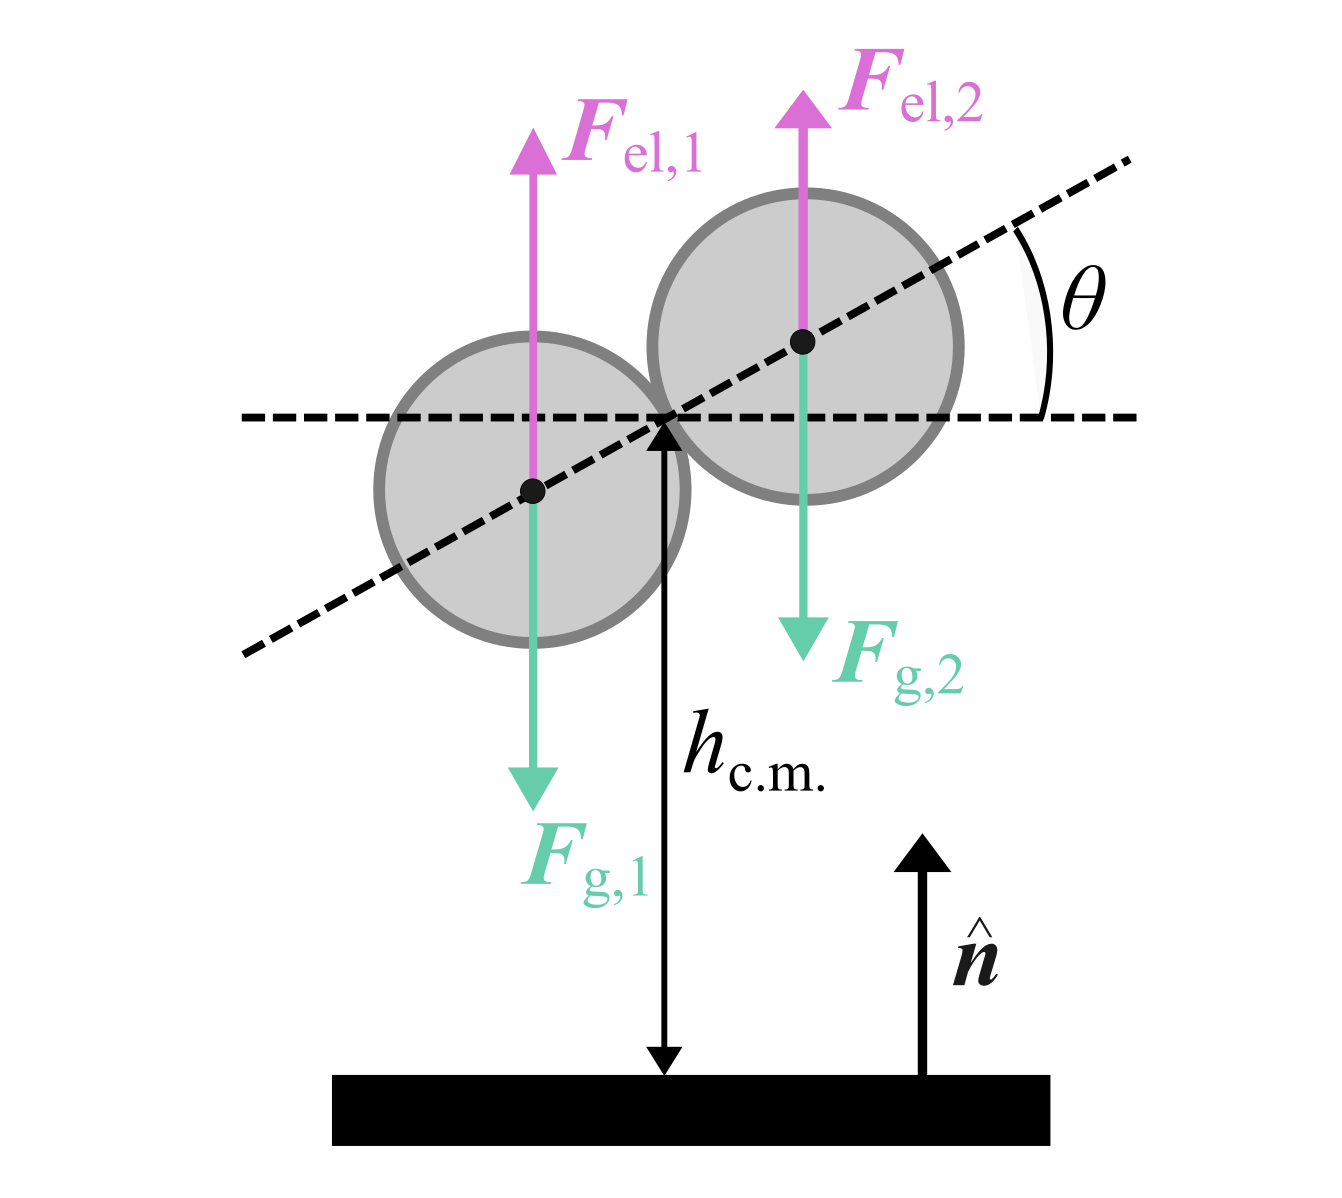
\includegraphics[width=0.4\linewidth]{figures/dumbbell_forces.png}
    \caption{Schematic picture of a dumbbell, with the distance between the particle's centre of mass and the wall $h_{\textrm{c.m.}}$ and the angle between the dumbbell's symmetry axis and the wall's plane. There are two forces acting on each sphere $i\in \{ 1,2 \}$ -- the electrostatic force $\boldsymbol{F}_{\textrm{el,}i}$ and the gravitational force $\boldsymbol{F}_{\textrm{g,}i}$. They respectively point in the direction opposite and along the wall-normal unit vector $\hat{\boldsymbol{n}}$.}
    \label{fig:dumbbell_forces}
\end{figure}

As suggested by the authors of Ref. \cite{verweij2021}, each sphere of index $i$ is assumed to be influenced by two forces -- the gravitational force $\boldsymbol{F}_{\textrm{g,}i}$ and the electrostatic force $\boldsymbol{F}_{\textrm{el,}i}$. The first one is always pointing downward; its definition is intuitive, and it can be written as
\begin{equation}
    \boldsymbol{F}_{\textrm{g}} = -\frac{4}{3} \pi a^3 \left( \rho_p - \rho_f \right) g \hat{\boldsymbol{n}},
\label{eqn:gravitational_force}
\end{equation}
where $g$ is the gravitational acceleration, $a=d/2$ is the sphere radius, $\rho_p$ and $\rho_f$ are the particle and fluid densities, respectively. The wall-normal unit vector $\hat{\boldsymbol{n}}$ is pointing upwards, as in Fig. \ref{fig:dumbbell_forces}.

The latter force emerges due to overlapping electric double layers (EDL) of the sphere and the wall. We have already introduced simplified expressions for the wall's and particle's EDL potentials $\Psi_{\textrm{DH,w}}$ and $\Psi_{\textrm{DH,p}}$ in Eq. \eqref{eqn:edl_potential_wall} and \eqref{eqn:edl_potential_sphere}. However, when two EDLs come close enough and overlap each other significantly, an expression becomes more complicated. In fact, it was already evaluated in the original paper of Verwey and Overbeek \cite{verwey_overbeek_1948}. The electric repulsion force $\boldsymbol{F}_{\textrm{el,}i}$ on the sphere of index $i$ is given as
\begin{equation}
    \boldsymbol{F}_{\textrm{el,}i}(h_{\textrm{c.m.}}) = 64 \pi \varepsilon \kappa a \left( \frac{k_B T}{e} \right)^2 \textrm{tanh} \left( \frac{e \Psi_w}{4 k_B T} \right) \textrm{tanh} \left( \frac{e \Psi_p}{4 k_B T} \right) \textrm{exp} \left(- \kappa h_{\textrm{c.m}.,i} \right) \hat{\boldsymbol{n}},
\label{eqn:electrostatic_force}
\end{equation}
where $\varepsilon$ is the electric permittivity of water, $\kappa^{-1}$ is the Debye length, $e$ is the elementary charge, $\Psi_w$ and $\Psi_p$ are the Stern potentials of the wall and the spherical particle, respectively. Even though an exponent term looks familiar to the previous expressions of Eq. \eqref{eqn:edl_potential_wall} and Eq. \eqref{eqn:edl_potential_sphere}, the preceding terms were not present in these more straightforward formulas. The $\textrm{tanh}$ terms arise from the constraint of the constant surface potentials on the wall's and particle's surfaces. In particular, the hyperbolic tangent terms arise from the nonlinear relationship between the surface potential and the ion distribution in the electrolyte, which is described with the Gouy-Chapman theory \cite{gouy_1910,chapman_1913}. As the surface potential increases, simple linear terms cannot approximate the ionic concentration profile around the surface, whereas the $\textrm{tanh}$ form captures how the potential saturates for large values. However, it is worth keeping in mind that the assumption of the constant surface potentials is not always satisfied in realistic systems, and the above formula has its limitations \cite{verwey_overbeek_1948}.

The resultant force on a dumbbell particle is a sum of the four forces acting on two spheres individually, and the resultant torque is also the sum of the four individual torques, calculated with respect to the dumbbell's centre of mass. Knowing the forces and torques on the particle, one can calculate the dumbbell's potential energy $\phi(h_{\textrm{c.m.}}, \theta)$, which is 
\begin{equation}
    \phi(h_{\textrm{c.m.}}, \theta) = -2 F_\textrm{g} h_{\textrm{c.m.}} + \frac{2 F_\textrm{el}(h_{\textrm{c.m.}})}{\kappa} \cosh(\kappa a \sin \theta ),
\label{eqn:dumbbell_potential_energy}
\end{equation}
where $F_{\textrm{g}} = |\boldsymbol{F}_{\textrm{g,}1} + \boldsymbol{F}_{\textrm{g,}2}|$ and $F_{\textrm{el}}(h_{\textrm{c.m.}}) = |\boldsymbol{F}_{\textrm{el,}1}(h_{\textrm{c.m.}}) + \boldsymbol{F}_{\textrm{el,}2}(h_{\textrm{c.m.}})|$. Now, we can use the potential $\phi(h_{\textrm{c.m.}}, \theta)$ to calculate the expected height and orientation distributions. First, let's define the two-dimensional probability Boltzmann distribution $p(h_{\textrm{c.m.}}, \theta)$, given as
\begin{equation}
    p(h_{\textrm{c.m.}}, \theta) \sim K \textrm{exp}\left( -\frac{\phi(h_{\textrm{c.m.}}, \theta)}{k_{\textrm{B}}T} \right)
\end{equation}
where $K$ represents the particle-wall hard-core interaction potential, namely $K=1$ always when the particle is above the wall and $K=0$ in other cases. To obtain each of the one-dimensional probability distributions we need to integrate out the other degree of freedom. Then, the height distribution $p(h_{\textrm{c.m.}})$ and the rotational distribution $p(\theta)$ are given as
\begin{equation}
    p(h_{\textrm{c.m.}}) \sim \int_{-\pi/2}^{\pi/2} d\theta \cos\theta K \exp \left( -\frac{\phi(h_{\textrm{c.m.}}, \theta)}{k_B T} \right),
\label{eqn:dumbbell_height_distribution}
\end{equation}
\begin{equation}
    p(\theta) \sim \int_{a}^{\infty} dh_{\textrm{c.m.}} K \exp \left( -\frac{\phi(h_{\textrm{c.m.}}, \theta)}{k_B T} \right),
\label{eqn:dumbbell_orientation_distribution}
\end{equation}

The functions defined in Eq. \eqref{eqn:dumbbell_height_distribution} and \eqref{eqn:dumbbell_orientation_distribution} were the ones that authors of Ref. \cite{verweij2021} expected to observe in the experimental data. However, not all the results matched their expectations, which is described in the next Section.


\subsection{Results and interpretation}

The simple theory proposed by Verweij \textit{et al.} \cite{verweij2021} was confronted with the experiment's results. The cyan histogram in the left panel of Fig. \ref{fig:dumbbell_experimental_distributions} represents the measured particle-wall separations $h_{\textrm{c.m.}}$, while the black line corresponds to $p(h_{\textrm{c.m.}})$ of the Eq. \eqref{eqn:dumbbell_height_distribution}. Comparing the histogram and the curve, one can see that the relatively simple theory can accurately predict the true distribution $p(h_{\textrm{c.m.}})$. However, an inset plot of Fig. \ref{fig:dumbbell_experimental_distributions}a suggests that there might be some differences between the results and the authors' theoretical model. For every dumbbell of $\theta \neq 0^{\circ}$, one can specify the lower (L, orange) and the upper (U, grey) sphere. The gap heights $h_{\textrm{g}}$ for the lower and upper spheres seem to be smaller and larger than expected, respectively. This means that the particles might be oriented more normally to the wall than the authors expected.

\begin{figure}
    \begin{minipage}{\linewidth}
         \centering
         \textbf{a)}
         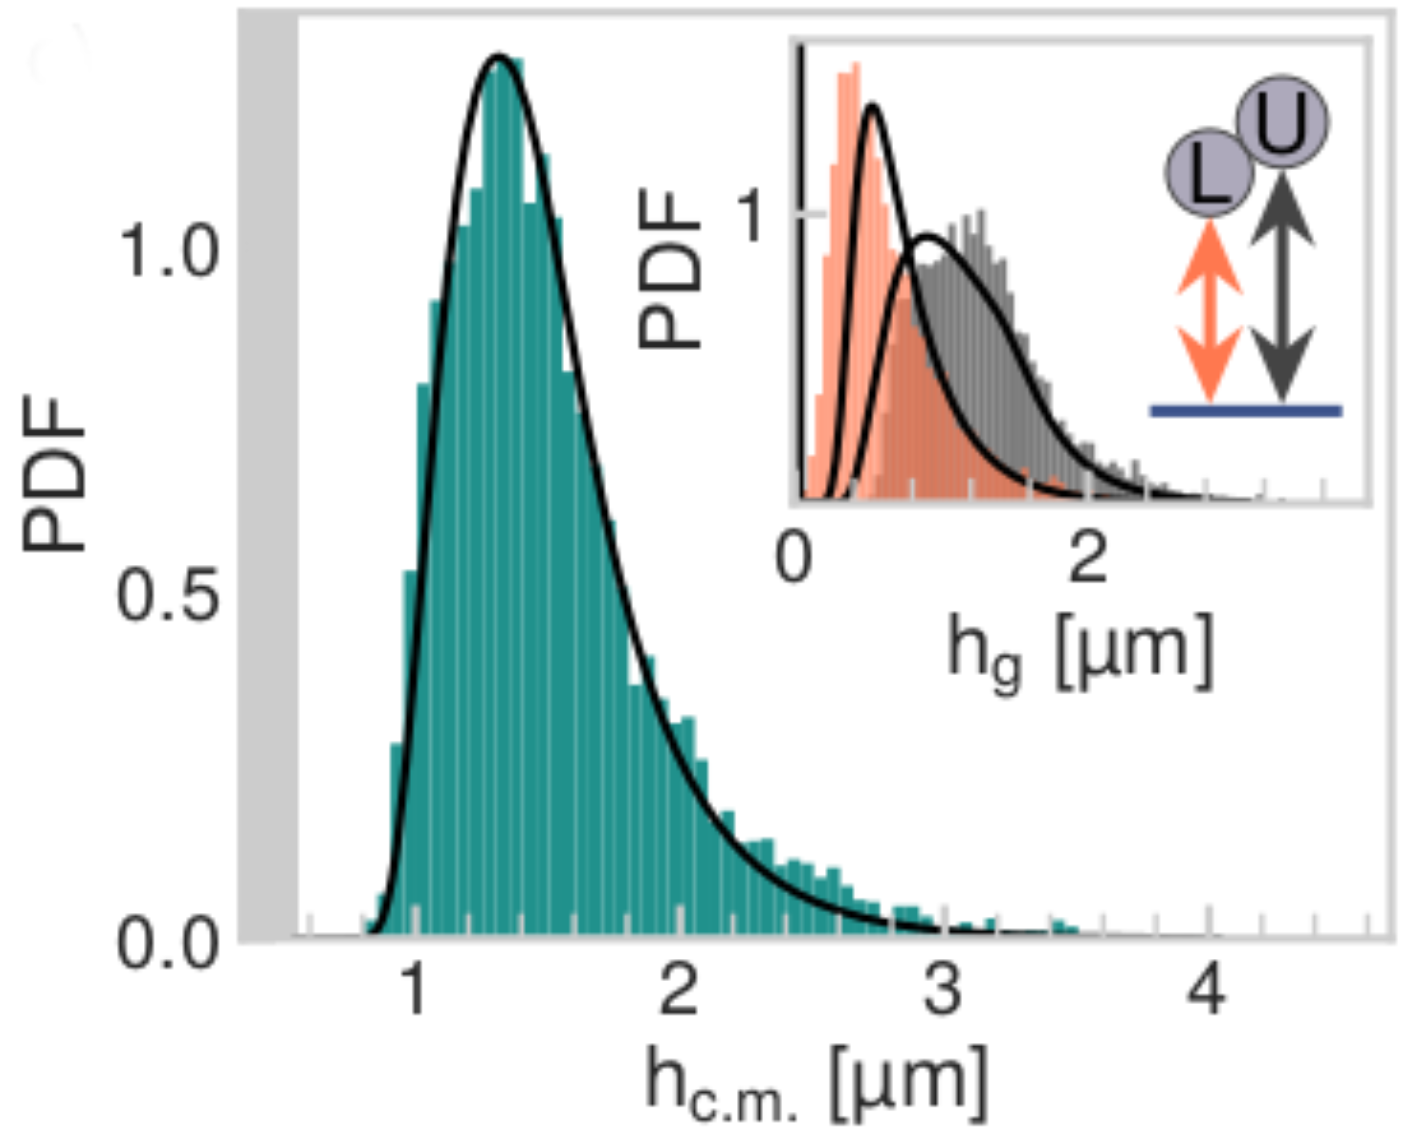
\includegraphics[width=0.45\linewidth,valign=t]{figures/small_dumbbell_heights.png}
         \textbf{b)}
         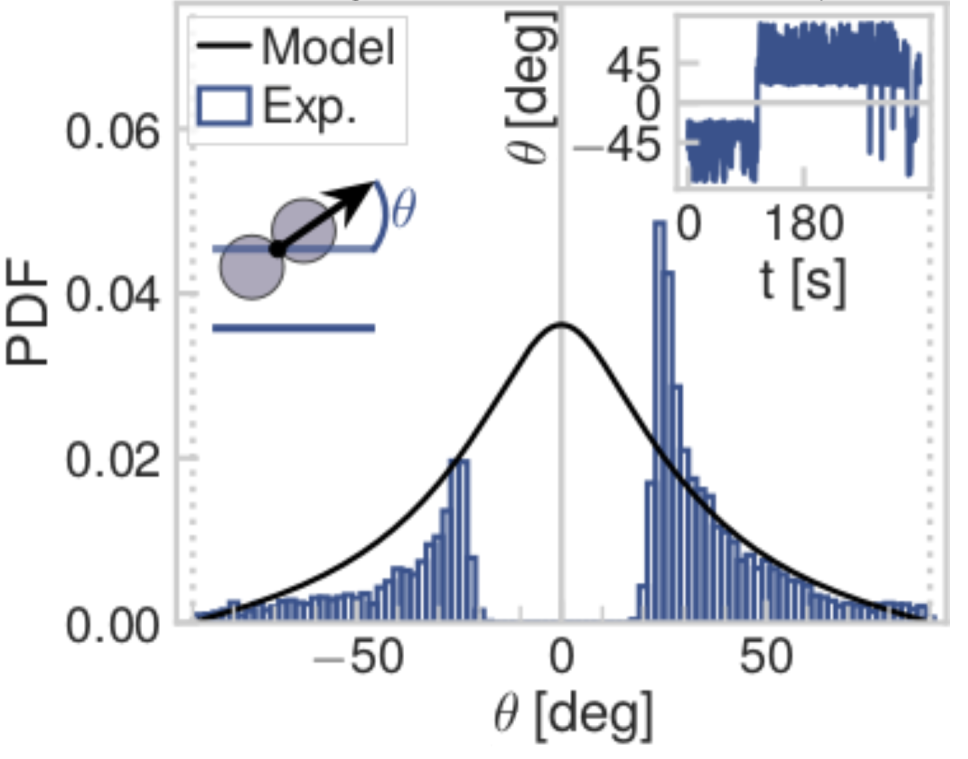
\includegraphics[width=0.45\linewidth,valign=t]{figures/small_dumbbell_orientations.png}
    \end{minipage}
    \caption{
    \textbf{a)} Histogram of the measured centre of mass heights $h_{\textrm{c.m.}}$ (green) and their expected distribution of Eq. \eqref{eqn:dumbbell_height_distribution} (black line). In the right-upper corner inset there are histograms of the measured gap height $h_{\textrm{g}}$ for the lower (orange) and the upper (grey) spheres, while black lines are their forecasted distributions. 
    \textbf{b)} Histogram of measured dumbbell angular orientations and the predicted distribution provided by the Eq. \eqref{eqn:dumbbell_orientation_distribution}. The inset plot shows a sample time $t$ evolution of a single particle's angle $\theta$. All the presented results apply to the $\sim 6$ minute trajectory of a single dumbbell of sphere diameter $d=1.10$ $\mu$m. Attribution: Verweij \textit{et al.} \cite{verweij2021} (Fig. 3c and 4b). These plots are directly reproduced from the original source.
    }
\label{fig:dumbbell_experimental_distributions}
\end{figure}

The deviating gap heights suggest investigating the particle angular orientations $\theta$ in more detail. Indeed, the right panel of Fig. \ref{fig:dumbbell_experimental_distributions} shows a striking discrepancy between the histogram of measured angles and the forecasted distribution $p(\theta)$ from the Eq. \eqref{eqn:dumbbell_orientation_distribution}. While the wall-parallel orientations are expected to be the most present, none was observed for the small particles of $d=1.10$ $\mu$m. Instead, the dumbbells were observed to be mainly oriented between the angles $25^{\circ}$ and $56^{\circ}$. Therefore, the true potential of the dumbbell energy must have some minimum in such an arrangement that one of the spheres is distinctly closer to the wall than the other one.

Moreover, in the inset of Fig. \ref{fig:dumbbell_experimental_distributions}b, the authors present a time evolution of $\theta$. In fact, all the presented histograms were calculated for this single trajectory. As one can see, the particle drastically changes its orientation to the other sign of $\theta$, which requires transition through the $0^{\circ}$ angle. However, the change is so rapid that none of the particles are captured in the middle of transition. With the relatively coarse measurement timescales $\Delta t\simeq 0.053$ s, rapid changes have indeed a low chance of being observed.

The scientists not only observed an unexpected dumbbell-twisting force but also noticed its variability with the particle size or length of particle-wall separation distances. As depicted in Fig. \ref{fig:dumbbell_KDEs}, for the bigger particles of $d=2.10$ $\mu$m the dumbbells tend to configurations that are closer to $\theta=0^{\circ}$ than it was for $d=1.10$ $\mu$m. The plots show the observed configurations of parameters ($h_{\textrm{c.m.}}, \theta$) for the smaller (a) and bigger (b) dumbbells used in the experiment. Each blue circle represents a single observation. The dashed black lines are the isolines of the distributions' kernel density estimations (KDE). The red area in the left panel is the geometrically restricted area -- to realise a configuration from this region, a dumbbell would need to penetrate the wall. Comparing these two plots, it is clear that the larger dumbbells are either less susceptible to the twisting effect or experience a smaller magnitude of this unknown torque. Whereas the maximum of smaller particles KDE lies around $\sim 32^{\circ}$, for the larger ones, it is $\sim 6^{\circ}$, and there was even no observation for which $\theta$ exceeded $30^{\circ}$. The values of $h_{\textrm{c.m.}}$ are also significantly different. While the smaller particles approach the wall at values comparable with $1/\kappa$ and sometimes nearly touch the boundary, the geometrically forbidden red area is even non-present in the scope of Fig. \ref{fig:dumbbell_KDEs}b.

\begin{figure}
    \begin{minipage}{\linewidth}
         \centering
         \textbf{a)}
         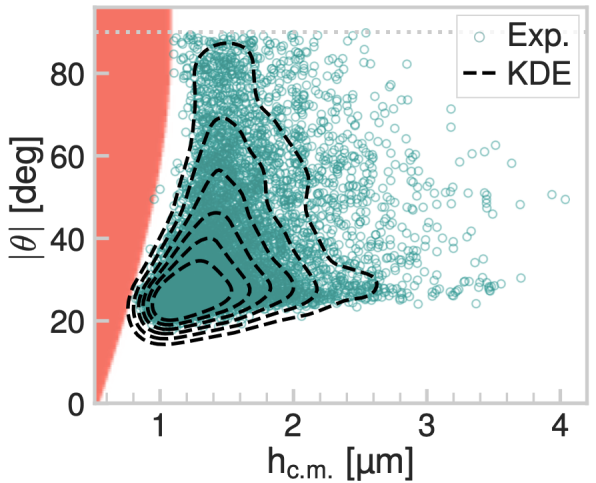
\includegraphics[width=0.45\linewidth,valign=t]{figures/small_dumbbells_KDE.png}
         \textbf{b)}
         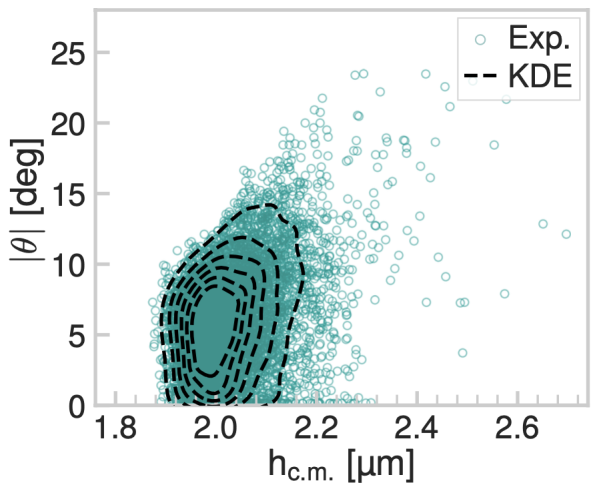
\includegraphics[width=0.45\linewidth,valign=t]{figures/big_dumbbells_KDE.png}
    \end{minipage}
    \caption{
    \textbf{a)} The distance-orientation configurations ($h_{\textrm{c.m.}}, \theta$) of each measurement (green circles) for the dumbbells of a sphere diameter $d=1.10$ $\mu$m. The black dashed lines represent chosen isolines of the kernel density estimations (KDE). The red area is the geometrically restricted region where the dumbbell would intersect the wall.  \textbf{b)} Analogous plot to the one in the left panel, presenting observations for the dumbbells of sphere size $d=2.10$ $\mu$m. Attribution: Verweij \textit{et al.} \cite{verweij2021} (Fig. 4c, 4f). The plots are directly reproduced from Ref. \cite{verweij2021}.
    }
\label{fig:dumbbell_KDEs}
\end{figure}

The reason why the twisting effect diminishes with the particle size can be twofold. One of the causes can be the growth of the particle's resistance. Even though the inertial effects are negligible in the Stokes regime, the dumbbell's mobility matrix can change with the growth of the sphere radius $a$. The second potential cause is the exponential nature of the EDL repulsion. The twisting effect might also quickly disappear since the EDL potentials decrease rapidly with growing $h_{\textrm{c.m.}}$. Both of these topics are investigated in detail in Section \ref{chapter:results}.

The striking discrepancy between the observed values of $\theta$ and the predictions of Eq. \eqref{eqn:dumbbell_orientation_distribution} was also discussed by the authors. However, they could not find a satisfactory explanation for this phenomenon. They suggest that the reason might be some higher-order electrostatic effects that they do not consider in their model. They do not exclude a more subtle interplay of other effects, such as buoyancy and hydrodynamics as well. However, before discussing possible developments of the theoretical model, we should focus on the potential shortcomings of the work of Verweij \textit{et al.} \cite{verweij2021}.


\subsection{Possible model improvements} \label{sec:shortcomings}

The experiment of Ref. \cite{verweij2021} is thoroughly described by the authors, and the setup was successfully tested for the simpler cases of spherical particles. The presented theoretical description is well-established, simple and straightforward. Given that, the observed non-parallel orientations are surprising and suggest the presence of potential shortcomings in the aforementioned work. In the rest of this Section, we will focus on the weaknesses of this publication.

When it comes to the experiment's preparation, the authors are using both the spherical particles grown by themselves (of radius $a=0.55$ $\mu$m) as well as the ones bought from the external supplier ($a=1.05$ $\mu$m). Even though the material is silicon dioxide in both cases, there is no guarantee that the potential differences in their manufacturing processes could not interfere with the experiment results. The spheres of each size had the same place of origin, however, the comparison between the results for smaller and larger dumbbells could be affected by this dissimilarity. Moreover, after obtaining the conglomerate of colloidal spheres and dumbbells in a thoroughly described electrolyte solution, the authors dissolved it in water multiple times without mentioning the exact volumes used. Finally, they obtained a $\textrm{pH} \sim 5.5$ solution of a very low ionic strength $I=3\times 10^{-6}$ M. The further estimations of the fluid properties could be more accurate if they were based not only on the measured $\textrm{pH}$.

The theory used to describe the observed particle's behaviour also contains a few crude simplifications. One of them is mentioned by the authors -- the electric interactions between a given sphere and a wall do not consider the presence of the second sphere and the resulting distortion of the electric double layers. The authors should have considered at least the simplest model of wall-mediated screening of the spheres, which we will explore further in Section \ref{sec:developments_results}. However, this is not the only simplification in the theory presented in Ref. \cite{verweij2021}. The Stern potentials of the spheres are approximated as equal to the surface potentials, and they are assumed to be constant, which is captured in Eq. \eqref{eqn:electrostatic_force}. Nonetheless, this assumption does not need to be accurate, especially in the regime of small particle-wall separations. Moreover, the authors assume that the Stern potentials are equal for both investigated spheres. Indeed, the unequal values of $\Psi_\textrm{p}$ could place the minimum energy configuration in the region of $\theta \neq 0^{\circ}$. It is also worth noticing that the Eq. \eqref{eqn:edl_potential_wall}, \eqref{eqn:edl_potential_sphere} and \eqref{eqn:electrostatic_force} are commonly considered as accurate for the ionic strengths larger than the experimental $I=3\times 10^{-6}$ M. The diffuse layer size (characterised by Debye length $1/\kappa$) should be significantly smaller than the particle size or measured particle-wall separations. However, for the smaller dumbbells of size $a$, we obtain $a \kappa \sim 3$, and a significant share of the observed values of $h_{\textrm{c.m.}}$ are of the order $\sim 3$ as well.

As we examine the observations, we notice that the time resolution of the measurements of Ref. \cite{verweij2021} is $\Delta t = 0.053$ s, which can be too coarse to observe some phenomena. Indeed, the experimental setup could not capture any of the $\theta=0^{\circ}$ configurations of smaller dumbbells. The wall-parallel orientations are necessary to perform a change of sign of $\theta$ depicted in the inset of Fig. \ref{fig:dumbbell_experimental_distributions}b and in Fig. \ref{fig:dumbbell_shortcomings}a, which analyse the same trajectory of a chosen particle. In fact, we could even hypothesise whether the shift through $\theta=0^{\circ}$ was actually performed. The post-processing of the measurement frames was not much focused on the distinction between each sphere and the exchange of indices $i$ could happen if the $z$-position of each sphere remained the same between the two frames, while the $x,y$-coordinates of each sphere would coincidentally exchange with the values of the previous frame. This topic cannot be explored in more detail with such a coarse time resolution. The left panel of Fig. \ref{fig:dumbbell_shortcomings} shows how the gap heights $h_{\textrm{g}}$ between the dumbbell's spheres and the wall change in time for a single selected trajectory. In this plot, a rapid shift in the orientation is again observed at times $t \sim 110$ s and $t\sim 340$ s. It is truly surprising that even though the example particle experienced the orientation shift twice, the researchers could not capture any transition through $\theta=0^{\circ}$ for numerous dumbbells that they measured. However, we see that the depicted trajectory is very ragged, highlighting the stochastic nature of the equations of motion and the difficulty of capturing the motion with such a large $\Delta t$.

\begin{figure}
    \begin{minipage}{\linewidth}
         \centering
         \textbf{a)}
         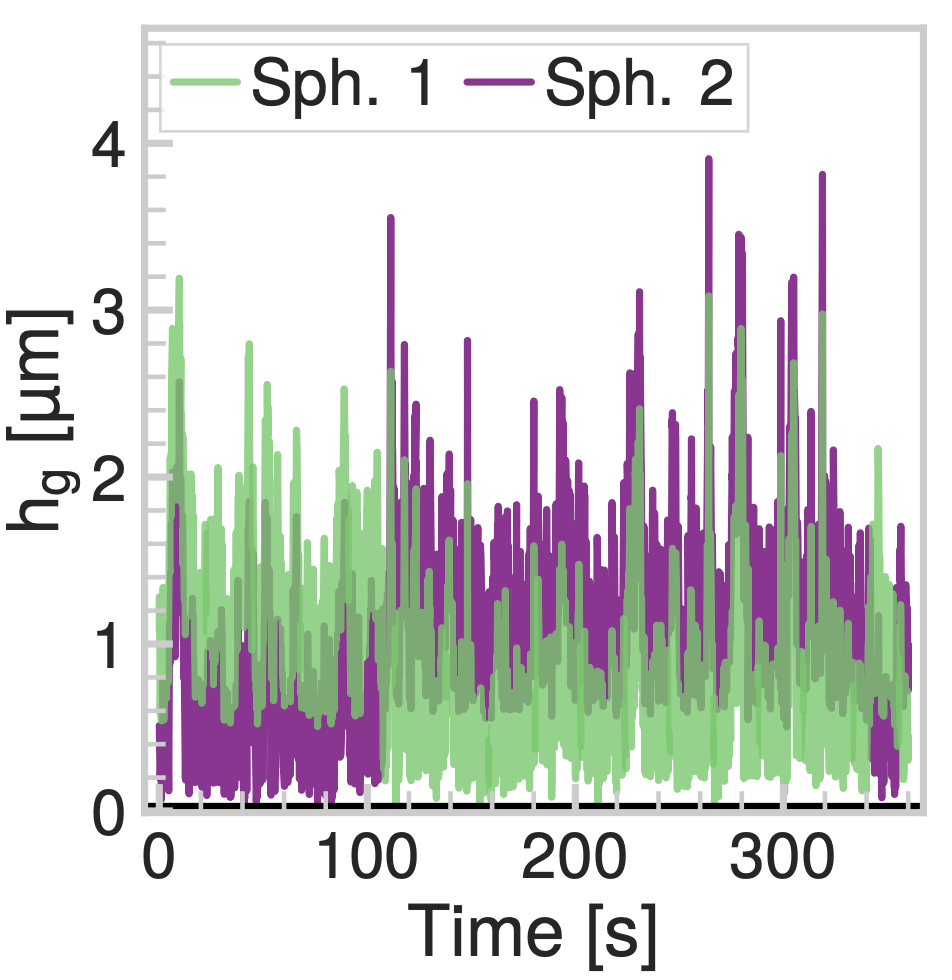
\includegraphics[width=0.395\linewidth,valign=t]{figures/small_dumbbell_trajectory.png}
         \textbf{b)}
         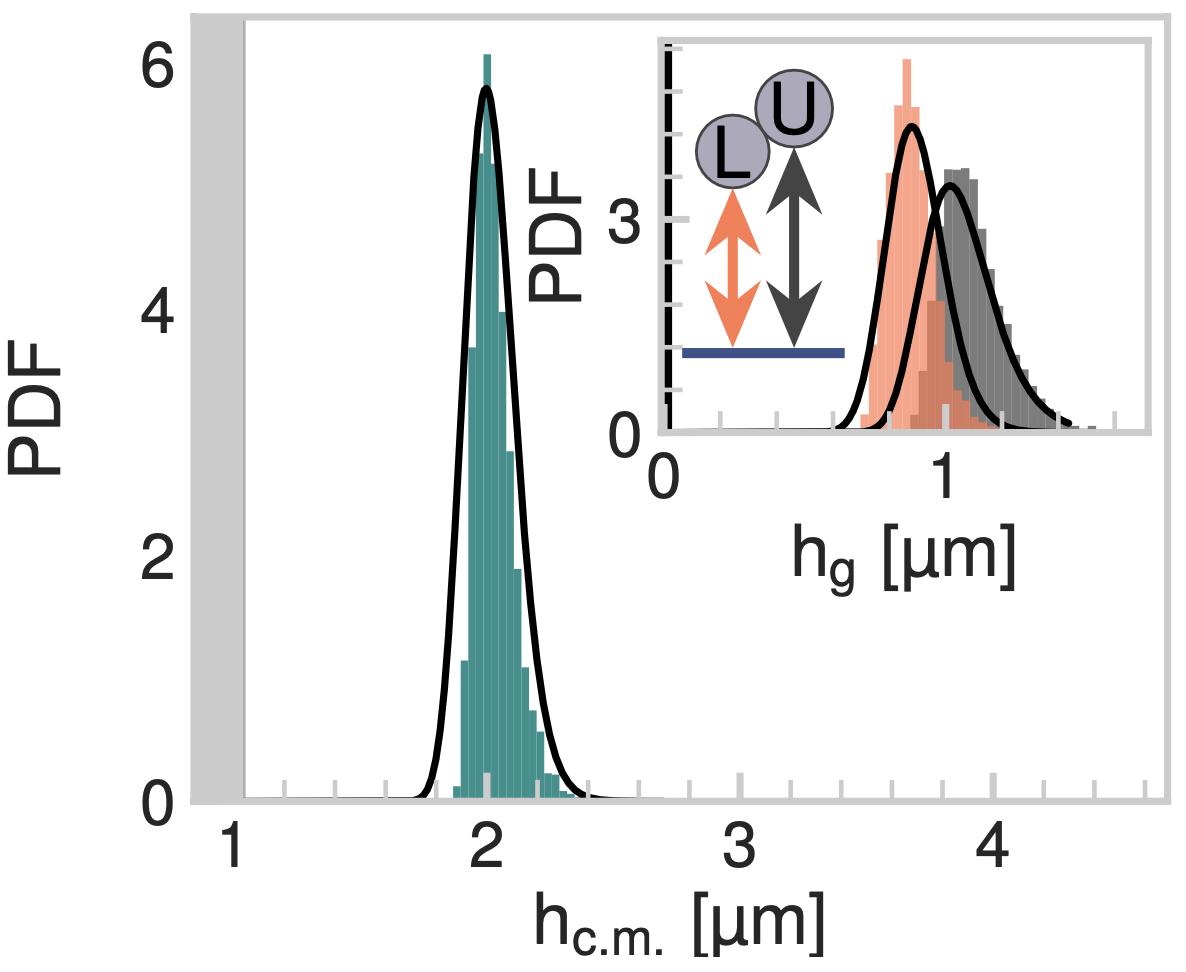
\includegraphics[width=0.5\linewidth,valign=t]{figures/large_dumbbells_heights.png}
    \end{minipage}
    \caption{
    \textbf{a)} Gap heights $h_\textrm{g}$ of a single dumbbell's trajectory, split between each of the two spheres -- Sph. 1 (green) and Sph. 2 (violet).
    \textbf{b)} Histogram of the measured centre of mass heights $h_{\textrm{c.m.}}$ (green) and their expected distribution of Eq. \eqref{eqn:dumbbell_height_distribution} (black line). In the inset, there are histograms of the measured gap height $h_{\textrm{g}}$ for the lower (orange) and the upper (grey) spheres, while black lines are their forecasted distributions, based on Eq. \eqref{eqn:dumbbell_height_distribution}. Attribution: Verweij \textit{et al.} \cite{verweij2021} (Fig. 3b, 3f). The plots are directly reproduced from Ref. \cite{verweij2021}.
    }
\label{fig:dumbbell_shortcomings}
\end{figure}

Finally, Fig. \ref{fig:dumbbell_shortcomings}b shows the histogram of the measured wall-particle separations $h_{\textrm{c.m.}}$ of the larger dumbbells and the fit (black line) of the Eq. \eqref{eqn:dumbbell_height_distribution} to this data. Although in Fig. \ref{fig:dumbbell_experimental_distributions}, the smaller dumbbell histogram and the curve align perfectly, we can not say this about the plot for the larger particles. This higlights another concern in Ref. \cite{verweij2021} -- the black curves of probability distributions $p(h_{\textrm{c.m.}})$ and $p(\theta)$ (Eq. \eqref{eqn:dumbbell_height_distribution} and \eqref{eqn:dumbbell_orientation_distribution}) are fitted to the measurements, with Debye length $1/\kappa$, particle density $\rho_p$ and particle's zeta-potential $\Psi_{\zeta \textrm{,p}}$ as the fit parameters. The density, which should be relatively easy to measure, varies from $2.0$ to $2.2$ g/cm$^3$. The values of $\Psi_{\zeta \textrm{,p}}$ are fitted as $-30$ mV and $-61$ mV for the smaller and larger dumbells, respectively. For the measurements of single spheres separations and the fitting of analogous versions of $p(h_{\textrm{c.m.}})$, Stern potential $\Psi_{\textrm{S,p}}$ is equal to $-41$ mV for smaller spheres and $-52$ mV for the bigger ones. Given that the electrostatic effects seem crucial in this system, such a disparity between the Stern potential values can be too large. The Debye length in the analysed fluid is estimated based on its $\textrm{pH}$. For the resulting ionic strength $I = 3 \times 10^{-6}$ M, the authors estimated $\kappa^{-1} = 0.304\textrm{ nm}/\sqrt{I} = 175$ nm. However, the four different fits result in $\kappa^{-1} \in \{ 103, 107, 207, 228 \}$ nm. Although the authors commented that these fitted values agree well with the primary estimate of $175$ nm, the disparity may be too large, given the sensitivity of $F_{\textrm{el}}(h_{\textrm{c.m.}})$ to $\kappa h_{\textrm{c.m.}}$. The impact of inconsistent values of both parameters $\Psi_{\textrm{S,p}}$ and $\kappa^{-1}$ is discussed in detail in Section \ref{sec:developments_results}.

Another doubt regarding the results of Ref. \cite{verweij2021} is the fact all the paper's plots (the majority of which is presented in Fig. \ref{fig:dumbbell_experimental_distributions}-\ref{fig:dumbbell_shortcomings}) involve only a single trajectory of either small or large dumbbell. A comparison with other trajectories could be beneficial in explaining the experiment results, at least to understand the possible inaccuracies of the measurements and explore the scope of possible evolution of the system's parameters.

All the points mentioned above are of a very different nature and refer to different aspects of Ref. \cite{verweij2021}. Most of them highlight the oversimplification of the electrostatic interactions model, as well as too arbitrary choice of values of $\kappa^{-1}$, $\rho_p$ and $\Psi_{\textrm{S,p}}$. The fits of the probability distributions $p(h_{\textrm{c.m.}})$ and $p(\theta)$ might seem to agree with the results thanks to the aforementioned fitting of relatively constant values -- this could cover the incapability of the measurement setup to capture more subtle phenomena in the system. The abovementioned doubts are thoroughly discussed in Section \ref{sec:developments_results}.

\chapter{Methodology} \label{chapter:methodology}

\section{Numerical mobility matrix solver -- \code{HYDROMULTIPOLE}} \label{sec:methodology:hydromultipole}

To accurately simulate the chosen particle's motion, we need to find the values of its mobility coefficients. For this, we can use the \code{HYDROMULTIPOLE} code \cite{cichocki2000}, which provides precise numerical approximations of $\bm{\mu}$ for the particles of a chosen size and shape, especially the ones constructed out of a few spheres joined together, in the vicinity of a wall. In fact, the simplest example of such an arrangement is a dumbbell shape. The code employs the approach presented in Section \ref{sec:hydrodynamics_theory} -- the force density and velocity field are rewritten in terms of the multipolar solutions to find the friction matrix $\mathsfbi{Z}$ of a colloidal particle constructed of $N$ spherical particles. Then, examining the wall's contribution is evaluated to find the particle's resistance matrix $\bm{\zeta}$. Then, it reverses the matrix to finally obtain $\bm{\mu}$. 

For the simple case of a sphere in an unbounded fluid body, its mobility matrix $\boldsymbol{\mu}_0$ is diagonal, and its coefficients can be divided into the translational $\mu^t_0$ and rotational $\mu^r_0$ ones, defined as
\begin{equation}
    \mu^t_0=\frac{1}{6\pi\eta a}, \qquad \mu^r_0=\frac{1}{8\pi\eta a^3},
\label{eqn:sphere_mobility_zero}
\end{equation}
where $\eta$ is the shear viscosity of a fluid. To show the high accuracy of \code{HYDROMULTIPOLE}, we can calculate all of the mobility coefficients of a single sphere approaching the wall at a given height $h_{\textrm{c.m.}}=a/t$. For such a relatively simple system, Cichocki and Jones \cite{cichocki1998} found the analytical exact expressions. Therefore, we can compare these two approaches, in particular, to evaluate the code's accuracy. Fig. \ref{fig:single_sphere_mobility} shows a comparison between the numerical findings (dashed lines) and the exact values (blue solid lines) of mobility. Then, for $t\rightarrow 0$, which represents configurations very far from the wall, the mobility matrix tends to $\bm{\mu}_0$. All plotted coefficients are normalised by their equivalents in the infinite case ($\mu^t_0$ and $\mu^r_0$), and therefore, the mobility curves tend to $1$ as $t\rightarrow 0$. The only exception is the translation-rotation coupling mobility $\mu^{\textrm{tr}}$ -- since its value at $h_{\textrm{c.m.}}\rightarrow \infty$ is equal to zero, it is normalised by $\sqrt{\mu^t_0 \mu^r_0}$. The tilde over the coefficients states that they are normalised.



Since the system contains multiple symmetries, the mobility matrix can be constructed from 5 different coefficients. In the LAB frame of reference (see Fig. \ref{fig:wr_frame}) these coefficients, after normalisation, are: translational wall-normal $\tilde{\mu}_z^{\textrm{t}}$ and wall-parallel mobility $\tilde{\mu}_x^{\textrm{t}}=\tilde{\mu}_y^{\textrm{t}}$, rotational wall-normal $\tilde{\mu}_z^{\textrm{r}}$ and wall-parallel mobility $\tilde{\mu}_x^{\textrm{r}}=\tilde{\mu}_y^{\textrm{r}}$, and the translation-rotation coupling $\tilde{\mu}^{\textrm{tr}}$. The nature of the first one is clearly $\sim 1 / h_{\textrm{c.m.}}$, and this is the fastest-decreasing diagonal coefficient. The translation directly towards the wall experiences the largest resistance from the fluid between the particle and the boundary. It is relatively easier to move parallel to the interface, as the curve of $\tilde{\mu}_x^{\textrm{t}}$ shows. The rotational mobilities are less susceptible to the change of $t$. Especially $\tilde{\mu}_z^{\textrm{r}}$ decays slowly as $t\rightarrow 1$, and contrary to the previous coefficients, it does not reach zero as the sphere touches the wall -- rotation around the $\hat{\boldsymbol{e}}$ vector does not violate the no-slip condition. The latter one relates the wall-parallel motion with the rotation around the wall-parallel vector. The translation-rotational mobility $\tilde{\mu}^{\textrm{tr}}$ occupies place of $a_{\textrm{tr}}$ and $b_{\textrm{tr}}$ in Eq. \eqref{eqn:mobility_tr}. Due to the system's symmetries, there is no coupling between $\hat{\boldsymbol{e}}_z$ translation and rotation. The curve of $\tilde{\mu}^{\textrm{tr}}$ is zero far from the wall, and it grows with the decreasing distance $h_{\textrm{c.m.}}$. However, its value is significantly smaller than the other mobilities and, therefore, does not impact the particle's actual motion much. Moreover, it also does not reach zero as the particle touches the wall -- a no-slip condition can be preserved with a wheel-like linked translation and rotation.

\begin{figure}
    \centering
    \includesvg[width=0.8\textwidth]{figures/sphere_mobility_comparison.svg}
    \caption{Mobility coefficients found numerically with \code{HYDROMULTIPOLE} (dashed lines) and analytical solutions (blue lines) from Ref. \cite{cichocki1998}. The translational and rotational mobilities are normalised by $\mu^t_0$ and $\mu^r_0$, respectively. The translation-rotation coupling coefficient $\tilde{\mu}^{\textrm{tr}}$ is divided by $\sqrt{\mu^t_0 \mu^r_0}$.}
    \label{fig:single_sphere_mobility}
\end{figure}

The methods investigated in Fig. \ref{fig:single_sphere_mobility} are based on different approaches and provide very similar results. Both of them take into account the lubrication effects, which are especially important in the low-separation regime. Besides the above comparison, the accuracy of \code{HYDROMULTIPOLE} was tested in multiple works, and this algorithm will be treated in the rest of this thesis as a source of the accurate estimations of $\bm{\mu}$.

\section{Numerical SDE solver -- \code{pychastic}} \label{sec:methodology_pychastic}

To effectively simulate the particle's behaviour close to a wall, we must solve its stochastic differential equations (SDE) of motion. While there are already some SDE-dedicated numerical packages available, \code{pychastic} is the one that operates in the user-friendly environment of Python. The package was presented in Waszkiewicz \textit{et al.} \cite{waszkiewicz2023}, where we already incorporated the results presented in Section \ref{sec:unbounded_results_sphere} into the publication as one of the examples of code's usage. The author of this thesis is one of the paper's co-authors, which allowed us to swiftly adjust the algorithms to some special cases and naturally, this dissertation can be perceived as one of the packages use cases.

Similarly to other SDE solvers, in \code{pychastic} we employed the Itō's approach, described in Section \ref{sec:sde_theory}. The change $\boldsymbol{dx}$ of a simulated variable $\boldsymbol{x}$ in a time $t$ and after a time step $dt$ is, as in Eq. \eqref{eqn:sde_general}, split into the drift term $\boldsymbol{a}(\boldsymbol{x}(t),t)$ and the noise term $\boldsymbol{b}(\boldsymbol{x}(t),t)$, driven by a Wiener process $\boldsymbol{dW}$. While the simulation of the deterministic part is straightforward and does not require any special integration methods, the stochastic part must be treated cautiously. We can rewrite it in terms of the Taylor-Itō expansion, considering its first three terms (see Eq. 6-9 in Ref. \cite{waszkiewicz2023}). \code{Pychastic} offers three different integration schemes that take the first, first two or first three terms of the Taylor-Itō expansion. They are of the strong order $1/2$, $1$ and $3/2$, respectively, named Euler, Milstein, and Wagner-Platen. Given the nature of our simulations, the Euler scheme provided sufficient accuracy, eliminating the need for more complex integration methods.

Another advantage of \code{pychastic} was that its creation process was connected with the research presented here. In fact, the \code{step\_post\_processing} function was created particularly for the case of Eq. \eqref{eqn:rotational_timestep} simulations. Since the coordinates $\boldsymbol{a} = (a_1,a_2,a_3)$ subspace is limited to $|\boldsymbol{a}|\in [0,\pi \rangle$, the equations need a check of a domain after each simulation time step. This feature is not always available in other SDE solvers and was not present in \code{pychastic} before the research presented here. Since this thesis was closely related to the development of the package, we could relatively easily obtain most of the results presented in Chapter \ref{chapter:results}. All the results presented below, if not stated differently, were obtained with the Euler algorithm and a time step $dt = 0.05$ s.

\chapter{Results} \label{chapter:results}

\section{Mobility matrix of a dumbbell particle} \label{sec:mobility_results}
To perform simulations of the dumbbell-shaped particle motion, first, we need to find the mobility matrix of such a body. Its mobility coefficients depend on the distance $h_{\textrm{c.m.}}$ between the particle's centre of mass and the wall, and the orientation -- an angle $\theta$ between the particle's symmetry axis and the wall's plane (see Fig. \ref{fig:dumbbell_forces}). In the case of axisymmetric particles, due to the system's various symmetries, the mobility matrix can be constructed of twelve $(h_{\textrm{c.m.}}, w)$-dependent elements, where $w=\cos\theta$ (see Eq. \eqref{eqn:mobility_tt} and \eqref{eqn:mobility_tr}).

Figure \ref{fig:dumbbell_mobilities_comparison} shows how every of these mobility coefficients depends on the scaled wall-particle distance $(1+w)t$ for a fixed angle $\theta = 45^{\circ}$, where $t=a/h_{\textrm{c.m.}}$. While the $t$ variable was enough to describe sphere's mobility in Fig. \ref{fig:single_sphere_mobility}, the dumbbell particle is elongated and the minimum distance $h_{\textrm{c.m.,min}}$ between the particle's centre of mass and the boundary changes with the changing $w$: $h_{\textrm{c.m.,min}}=a$ while dumbbell lies parallel to the wall, and $h_{\textrm{c.m.,min}}=2a$ for $w=0$. Therefore, we must apply a scaling factor of $(1+w)$ to make plots for different $w$ comparable with each other. The mobility matrix was calculated with the \code{HYDROMULTIPOLE} code and is expressed in the particle-fixed RW frame (see Fig. \ref{fig:wr_frame}), with each of the RW-axes $(\hat{\boldsymbol{u}}_1, \hat{\boldsymbol{u}}_2, \hat{\boldsymbol{u}}_3)$ indices expressed in the subscripts. For example, $\mu^{\textrm{tt}}_{12}$ describes the particle's mobility in the case of both forces pointing in the direction of $\hat{\boldsymbol{u}}_2$ and linear velocity along $\hat{\boldsymbol{u}}_1$. Each of the subplots of Fig. \ref{fig:dumbbell_dimensionless_mobilities_comparison} is separated into three regions. The white regions on the left-hand side represent the configurations where the particle is far away from the boundary, and its influence on the mobility is insignificant. The limit of $(1+w)t \rightarrow 0$ represents the unbounded fluid case, where the wall is infinitely far away from the particle. The second white region is the area of close proximity and the high influence of lubrication effects on the particle's motion. The case of $(1+w)t = 1$ is a configuration where the particle touches the wall. The grey region between these two represents typical particle-wall separations usually observed in experiments. The equilibrium between gravitational and electrostatic forces predominantly lies somewhere in this regime. In fact, the borders of grey areas were determined based on the distributions obtained in the experiment of Verweij \textit{et al.} \cite{verweij2021}. 

The top panel of Fig. \ref{fig:dumbbell_mobilities_comparison} shows how translational mobility coefficients change with the distance $h_{\textrm{c.m.}}$. Similarly to $\tilde{\mu}^{\textrm{t}}_z$ (see Fig. \ref{fig:single_sphere_mobility}), for most of the configurations, the translational mobility relations are $\sim t$ and only in the lubrication regime the curves deviate from linear behaviour. In fact, the wall's close proximity strongly influences the particle's mobility, and all the translational elements tend to zero as $h_{\textrm{c.m.}} \rightarrow (1 + w) a$. The three coefficients along the RW-axes are the largest far from the wall, whereas, in the limit of $h_{\textrm{c.m.}}\rightarrow\infty$, the mobility along the particle's symmetry axis is the largest. In the far field regime, there is nearly no coupling between motion in the directions $\hat{\boldsymbol{u}}_1$ and $\hat{\boldsymbol{u}}_3$. As the particle approaches the boundary, the wall's screening links the motion in these two directions together, even though they are normal to each other. This relation is determined by $\tilde{\mu}^{\textrm{tt}}_{13}$, which indeed grows with decreasing distance $h_{\textrm{c.m.}}$ but this quantity also reaches zero as the particle touches the boundary.

When it comes to the rotational mobility, the left panel shows that the mobility coefficients remain nearly constant and decay slowly with the distance's inverse, as for the simpler case of a single sphere. An interesting observation is the negative sign of $\tilde{\mu}^{\textrm{rr}}_{13}$ -- it means that i.e. clockwise rotation around $\hat{\boldsymbol{u}}_1$ results in an anti-clockwise torque in the direction of $\hat{\boldsymbol{u}}_3$. Whereas the rotational mobility in the RW axes is suppressed as the particle touches the wall, this is not the case of $\tilde{\mu}^{\textrm{rr}}_{13}$. This quantity is non-zero even when $h_{\textrm{c.m.}} = (1 + w) a$.

The right panel of Fig. \ref{fig:dumbbell_mobilities_comparison} shows the mobility coefficients for the coupling between translation and rotation. These quantities can be positive or negative. Contrary to the previous ones, they are zero infinitely far from the wall since there is no interaction that could bond the translation with rotation. They quickly alter as the dumbbell approaches the interface and often reach maximum mobility for the configuration where the particle and the barrier are in direct contact. Although these elements of the mobility matrix seem to be the most complex, their magnitude is much smaller than the tt or rr ones. In fact, they become significant only in the lubrication regime, which is not the subject of our further investigation.


\begin{figure}
    \centering
    \includesvg[width=\textwidth]{figures/dumbbell_mobilities_comparison.svg}
    \caption{Mobility coefficients of a dumbbell particle with an inclination angle $\theta=45^{\circ}$. The coefficients are grouped into specific types of motion coupling: translational (top panel), rotational (left) and translational-rotational (right). All of the plots are divided into three regions: far field, area of typically observed particle-wall separations and the lubrication regime. The results were found numerically with the \code{HYDROMULTIPOLE} code.}
    \label{fig:dumbbell_mobilities_comparison}
\end{figure}

Since the numerical finding of $\bm{\mu}$ can lead to singularities, a common approach is to first find the resistance matrix $\bm{\zeta}$ and then calculate its inverse. As discussed in Section \ref{sec:axisymmetric_mobility_theory}, each element of $\bm{\zeta}$ for an axisymmetric particle close to the wall can be approximated as a polynomial of the resistance matrix elements in an unbounded fluid $\bm{\zeta}_0$, height $h_{\textrm{c.m.}}$ and the trigonometric functions $\cos\theta = w$ and $\sin\theta = \sqrt{1 - w^2}$. These approximations were derived based on the approach presented in work of Lisicki \textit{et al.} \cite{lisicki2016} (in particular Eq. 6-9 in that work), and will be referred to as an analytical approach for the rest of this Section.

A comparison between the chosen mobility coefficients found numerically (dashed lines), and their polynomial approximations (solid lines) is depicted in Figure \ref{fig:dumbbell_dimensionless_mobilities_comparison}. Since the mobility coefficients depend on two parameters $h_{\textrm{c.m.}}$ and $w$, we can investigate the $h_{\textrm{c.m.}}$-dependence via putting the scaled particle-wall distance $(1+w)t$ on the x-axis, whereas the angle changes between three values: $\theta\in\{0^{\circ}, 45^{\circ}, 90^{\circ}\}$, for which $w\in\{ 1, \frac{1}{\sqrt{2}}, 0 \}$, presented in the left, middle and right panels of Fig. \ref{fig:dumbbell_dimensionless_mobilities_comparison}, respectively. The translational and rotational mobility coefficients are normalised by their values in an infinite space -- $\mu_{11,0}^{\textrm{tt}}$ and $\mu_{22,0}^{\textrm{rr}}$. Therefore, for $(1+w)t\rightarrow 0$ the normalised mobility values reach $1$. However, in the case of the translation-rotation coupling coefficient, its value is zero in the far field limit. Therefore, these coefficients are normalised by $\sqrt{\mu_{11,0}^{\textrm{tt}}\mu_{11,0}^{\textrm{rr}}}$, which is a combination of the far-field translational and rotational mobility along the particle's symmetry axis.

\begin{figure}
    \centering
    \includesvg[width=\textwidth]{figures/dumbbell_dimensionless_mobilities_comparison.svg}
    \caption{Chosen elements of the mobility matrix $\bm{\mu}(h_{\textrm{c.m.}}, w)$ of a dumbbell, calculated numerically (dashed lines) and approximated analytically (solid lines). The top panels show the translational mobility coefficient $\tilde{\mu}^{\textrm{tt}}_{11}$, the middle ones the rotational coefficient $\tilde{\mu}^{\textrm{rr}}_{22}$, and the bottom ones show the translation-rotation coupling mobility $\tilde{\mu}^{\textrm{tr}}_{23}$. Configurations in the left, middle and right panels were calculated for $w \in \{1, 1/\sqrt{2}, 0 \}$, respectively. The tt and rr coefficients were normalised by their values infinitely far away from the wall -- $\mu^{\textrm{tt}}_{11,0}$ and $\mu^{\textrm{rr}}_{22,0}$. The coefficient $\tilde{\mu}^{\textrm{tr}}_{23}$ was normalised by $\sqrt{\mu^{\textrm{tt}}_{11,0}\mu^{\textrm{rr}}_{11,0}}$.}
    \label{fig:dumbbell_dimensionless_mobilities_comparison}
\end{figure}

Looking at a chosen translational mobility coefficient $\tilde{\mu}_{11}^{\textrm{tt}}$, presented in the top panels, the analytical approximations are usually close to the accurate numerical results. The relative error (yellow line), calculated with respect to the numerical outcomes, is usually below $10\%$ for the region of typical wall-particle separations. The estimations of $\tilde{\mu}_{11}^{\textrm{tt}}$ are the most accurate when the dumbbell is oriented parallel to the wall. Here, the dumbell's spheres are within the same distance to the confinement. The analytical approach is the least accurate for the wall-normally oriented dumbbells. While $\tilde{\mu}_{11}^{\textrm{tt}}$ shows clear dependence on $h_{\textrm{c.m.}}^{-1}$, this coefficient does not change significantly with $w$.

An example of the rotational mobility is presented in the middle panels of Fig. \ref{fig:dumbbell_dimensionless_mobilities_comparison}, investigating the $(h_{\textrm{c.m.}}, w)$-dependence of the coefficient $\tilde{\mu}^{\textrm{rr}}_{22}$. Similarly to the translational mobility, the analytical approximations work well, with the relative error below $10\%$ for the region of typical separations. The particle's resistance to rotation is similar for both $\theta=45^{\circ}$ and $\theta=90^{\circ}$ cases. However, when the dumbbell is in the wall-parallel position, its mobility quickly drops as it approaches the boundary. In fact, a rotation around $\hat{\boldsymbol{u}}_2$ axis in this specific configuration ($\theta = 0^{\circ}$) results in the most significant possible change of the gap between the particle's surface and a wall, which can be the most influential parameter in this system.

The bottom panels of Fig. \ref{fig:dumbbell_dimensionless_mobilities_comparison} show how the translation-rotation coupling coefficient $\tilde{\mu}^{\textrm{tr}}_{23}$ depends on $h_{\textrm{c.m.}}$ and $w$. An interesting observation is that for $w=1$, there is no coupling between translation and rotation in these two directions. While the dumbbell is parallel to the wall, a movement along $\hat{\boldsymbol{u}}_2$ does not imply rotation around $\hat{\boldsymbol{u}}_3$, and vice versa. In this case we do not calculate a relative error. However, this is not the case for any other value of $w$. In the limiting case of the wall-normal orientation, both $\hat{\boldsymbol{u}}_2$ and $\hat{\boldsymbol{u}}_3$ are parallel to the wall, while the particle's symmetry axis is normal to its surface. In fact, it is easy to imagine such a particle moving along some specific direction and rotating around the other one, like a wheel that rotates due to direct contact with the ground.

The two proposed approaches differ primarily in the lubrication regime, which is not our current point of interest. For the separations typical to the ones observed in Ref. \cite{verweij2021}, the relative error is below $5\%$. Therefore, we can now rely on the approach proposed by Ref. \cite{lisicki2016} and possibly compare its further performance with \code{HYDROMULTIPOLE} again.

\section{Brownian motion in an unbounded fluid} \label{sec:unbounded_results}

\subsection{Spherical particle} \label{sec:unbounded_results_sphere}

Once we have found satisfying approximations of the mobility matrix $\bm{\mu}$, we can perform simulations of the colloidal particle's motion. Beginning with the simplest case of dynamics in an unbounded fluid, we first simulate the translational and rotational equations of motion, described by the Eq. \eqref{eqn:translational_timestep} and \eqref{eqn:rotational_timestep}, of a colloidal sphere of radius $a$. The SDE calculations were conducted with the use of the \code{pychastic} package and with the implementation of the algorithm proposed by Evensen \textit{et al.} \cite{evensen2008}. Even though the procedures of Ref. \cite{evensen2008} are clear and seem to be an efficient way to describe the evolution of a particle's angular orientation, throughout the research process, it turned out that some of the original equations contain typographical errors. Therefore, the results in Fig. \ref{fig:unbounded_sphere} are divided into the ones obtained with the original version of the equations presented in Evensen \textit{et al.} \cite{evensen2008} (violet), and the outcomes of our algorithm with the correct equations (green). Moreover, the Eq. \eqref{eqn:rotational_timestep} can become problematic around the polar orientations due to $\Phi=0$ and consequent division by zero. Therefore, one should apply the Taylor expansion for $\Phi\simeq 0$. This was already performed by Ilie \textit{et al.} \cite{ilie2014}; however, this work also contains some typos. Our algorithm is based on both works of Ref. \cite{evensen2008,ilie2014}, with the errors fixed. The differences between all the original and corrected equations are rather technical; therefore, they are not presented in this thesis. For the exact formulae, one should look into the work of Waszkiewicz \textit{et al.} \cite{waszkiewicz2023}, in particular Appendix B.

To evaluate the performance of both algorithms, we can investigate whether the system tends to any equilibrium distribution and what it looks like. For the spherical particle, an equilibrium distribution probability density $P^{\textrm{eq}}(\Phi)$ is given as
\begin{equation}
    P^{eq}(\Phi)=\frac{1-\cos\Phi}{\pi},
\label{eqn:equilibrium_probability}
\end{equation}
where $\Phi$ is the rotation vector, already introduced in Section \ref{sec:evensen_theory}. The left panel of Fig. \ref{fig:unbounded_sphere} shows that both of the algorithms tend to the same equilibrium distribution -- both violet histogram for Evensen \textit{et al.} \cite{evensen2008} and green histogram for the algorithm with correct equations align with the black curve of $P^{\textrm{eq}}(\Phi)$.

Even though the stationary distribution agrees with the predictions, we can investigate the dynamic properties of the solution in more detail. Cichocki \textit{et al.} \cite{cichocki2015} have found how the correlations of the modified rotation vector components $\Delta u_k(t) = - \frac{1}{2} \epsilon_{ijk} \Omega_{ij}(t)$ change in time $t$, which is often a great measure to evaluate the performance of colloidal dynamics simulations. These correlations are defined as
\begin{equation}
    \langle \Delta u_k (t) \Delta u_l (t) \rangle_0 = \left[
    \frac{1}{6} - \frac{5}{12}e^{-6D_r t} + \frac{1}{4}e^{-2D_r t}
    \right] \delta^{K}_{kl},
    \label{eqn:correlations_sphere}
\end{equation}
where $\delta^{K}_{kl}$ is the Kronecker delta and $D_r=k_BT/8\pi\eta a^3=k_BT\mu_0^{\textrm{r}}$ is the rotational diffusion coefficient of a spherical particle. Here, the disparity between the violet and green results is significant, as shown in the right panel of Fig. \ref{fig:unbounded_sphere}. There are three curves for each method since the correlations $\langle \Delta u_k (t) \Delta u_l (t) \rangle_0$ can be calculated with respect to three different axes. All three results align with each other for both versions of the algorithm, and both approaches resemble a similar shape. However, the violet shape is more compact than the green one -- the approach of Evensen \textit{et al.} \cite{evensen2008} tends to the equilibrium state significantly quicker than our corrected algorithms.

\begin{figure}
    \centering
    \includesvg[width=\linewidth]{figures/unbounded_sphere.svg}
    \caption{\textbf{Left:} Probability density functions after significant time $t>2$ of simulations for both of the original algorithm of Evensen \textit{et al.} \cite{evensen2008} and our correct equations version. The black line is the expected symmetric solution, described with Eq. \eqref{eqn:equilibrium_probability}. \textbf{Right:} Time evolution of the correlations of the modified rotation vector components. The violet lines are based on Ref. \cite{evensen2008} algorithm, the green ones are the correct equations version. The dashed line is the analytical solution found by Cichocki \textit{et al.} \cite{cichocki2015}, described in the Eq. \eqref{eqn:correlations_sphere}.}
    \label{fig:unbounded_sphere}
\end{figure}

As presented, both of the algorithms achieve the same equilibrium distribution $P^{\textrm{eq}}(\Phi)$ after a given time, which in our case, is $t>2$. However, the simulations differ notably before reaching the stationary state due to few typos in the original equations of Evensen \textit{et al.} \cite{evensen2008}. In fact, the authors have compared their results with $P^{\textrm{eq}}(\Phi)$. However, they did not perform a more in depth analysis analogous to the one on the right panel of Fig. \ref{fig:unbounded_sphere}. This highlights a need for better design of test cases that reliably test the proposed algorithm.

Once we are sure about our description of the particle's angular position evolution, we can apply the same approach to the dumbbell shape.

\subsection{Dumbbell particle}

Once we have found an algorithm that can accurately describe the motion of a colloidal sphere, we can use it to investigate the motion of dumbbell-shaped particles. The only significant difference compared to the previous simulations is a change in the mobility matrix. When there is a lack of any wall, the translational and rotational mobility matrices $\bm{\mu}^{tt}_{\textrm{db},0}$, $\bm{\mu}^{rr}_{\textrm{db},0}$ of a dumbbell are approximately equal to
\begin{equation}
    \bm{\mu}^{tt}_{\textrm{db},0} \simeq 
    \begin{pmatrix}
        0.26 & 0 & 0\\
        0 & 0.23 & 0\\
        0 & 0 & 0.23
    \end{pmatrix} \frac{1}{6 \pi \eta a},
    \qquad
    \bm{\mu}^{rr}_{\textrm{db},0} \simeq 
    \begin{pmatrix}
        0.55 & 0 & 0\\
        0 & 0.27 & 0\\
        0 & 0 & 0.27
    \end{pmatrix} \frac{1}{8 \pi \eta a^3},
\label{eqn:unbounded_dumbbell_mobility}
\end{equation}
where the values in the denominators are the mobility coefficients of a single sphere in the unbounded fluid case (see Eq. \eqref{eqn:sphere_mobility_zero}). The approximated numerical values of Eq. \eqref{eqn:unbounded_dumbbell_mobility} were found with the \code{HYDROMULTIPOLE} code, taking the limit of $h_{\textrm{c.m.}}\rightarrow \infty$.

With the new mobility coefficients, we can employ the same algorithm for the colloidal sphere by changing the values of $\bm{\mu}$ in the equations. The sample trajectories of a dumbbell, simulated with \code{pychastic}, are shown in the left panel of Fig. \ref{fig:unbounded_dumbbell}. All plotted curves are significantly ragged, highlighting the stochastic nature of the colloidal particle motion. Since any geometrical confinement does not bound the motion, the three green-blue Cartesian variables describing the particle's centre of mass position ($x_{\textrm{c.m.}}$, $y_{\textrm{c.m.}}$, $z_{\textrm{c.m.}}=h_{\textrm{c.m.}}$) can freely evolve, with their expected value equal to zero (see Section \ref{sec:sde_theory}). However, the particle's angular orientation $\theta$ (blue line) is limited to $[-\pi/2, \pi/2\rangle$, which is emphasised with two dashed orange lines in Fig. \ref{fig:unbounded_dumbbell}. 

\begin{figure}
    \centering
    \includesvg[width=\linewidth]{figures/evensen_comparison_dumbbell.svg}
    \caption{\textbf{Left:} Example time $t$ evolution of the position of the dumbbell particle's centre of mass, described with three Cartesian coordinates $x_{\textrm{c.m.}}$, $y_{\textrm{c.m.}}$, $z_{\textrm{c.m.}}=h_{\textrm{c.m.}}$ and the angular orientation $\theta$. \textbf{Right:} Modified rotation vector components' correlations $\langle \Delta u_k (t) \Delta u_l (t) \rangle_0$. The solid lines represent analytically-found correlations (see Eq. \eqref{eqn:correlations_dumbbell_symmetry} and \eqref{eqn:correlations_dumbbell_normal}), whereas dots are the results obtained for the simulations of a $10^4$ dumbbell-shaped colloidal particles ensemble.}
    \label{fig:unbounded_dumbbell}
\end{figure}

The right panel of Fig. \ref{fig:unbounded_dumbbell} shows the time evolution of the modified rotation vector components, analogous to the ones for the sphere in Fig. \ref{fig:unbounded_sphere}. However, the dumbbell particle is less symmetric. Therefore, it has two different values of rotational diffusion coefficient -- first one $D_1$ along the particle's symmetry axis and the second one $D_2=D_3$ in the directions normal to $\hat{\boldsymbol{u}}_1$. The correlations $\langle \Delta \bm{u} (t) \Delta \bm{u} (t) \rangle_{0}$ are described with two different equations, depending on the choice of the axis. For the symmetry axis \cite{cichocki2015}, they are given as
\begin{equation}
    \langle \Delta u_1(t) \Delta u_1(t) \rangle_{0} = \frac{1}{6} + \frac{1}{12}e^{-6 D_3 t} - \frac{1}{2}e^{-(2 D_3 + 4 D_1)t} + \frac{1}{4}e^{-2 D_3 t},
\label{eqn:correlations_dumbbell_symmetry}
\end{equation}
whereas for $\hat{\boldsymbol{u}}_2$ and $\hat{\boldsymbol{u}}_3$ \cite{cichocki2015} they can be described with
\begin{equation}
    \langle \Delta u_2(t) \Delta u_2(t) \rangle_{0} = \langle \Delta u_3 (t) \Delta u_3 (t) \rangle_{0} = \frac{1}{6} - \frac{1}{6}e^{-6 D_3 t} - \frac{1}{4}e^{-5(D_3 + D_1)t} + \frac{1}{4}e^{-(D_3 + D_1)t}.
\label{eqn:correlations_dumbbell_normal}
\end{equation}

Both of the curves are plotted in the right panel of Fig. \ref{fig:unbounded_dumbbell} -- Eq. \eqref{eqn:correlations_dumbbell_symmetry} with the green solid line, Eq. \eqref{eqn:correlations_dumbbell_normal} with the violet one, both referred to as the analytical expressions. The numerical results, represented with dots, again align with the predictions of Ref. \cite{cichocki2015}. The simulation data was averaged over a relatively small ensemble of $10^4$ dumbbell particles. For larger collectives, the lines and dots overlap and become indistinguishable. Since simulations of a relatively low computational cost can produce satisfying results, we can make the system more complex. In particular, we can introduce the wall by implementing a model of particle-wall interactions.


\section{Reconstruction of the experiment with a wall} \label{sec:verweij_results} \label{sec:wall_results}

To better understand and further investigate the surprising behaviour of colloidal dumbbells near the wall presented in Ref. \cite{verweij2021}, we can recreate the theoretical model of the authors, defined in Section \ref{sec:verweij_theory}. For the case of an unbounded fluid body, Eq. \eqref{eqn:translational_timestep} and \eqref{eqn:rotational_timestep} describe the system satisfactorily, as shown in the previous Section. To add the wall's influence, we need to supplement the equations of motion with the gravitational force $\boldsymbol{F}_\textrm{g}$ and the electrostatic repulsion force $\boldsymbol{F}_\textrm{el}$, described in Eq. \eqref{eqn:gravitational_force} and \eqref{eqn:electrostatic_force}, as well as the resulting torque. Therefore, the total force $\boldsymbol{F} = \boldsymbol{F}_{\textrm{g,}1} + \boldsymbol{F}_{\textrm{g,}2} + \boldsymbol{F}_{\textrm{el,}1} + \boldsymbol{F}_{\textrm{el,}2}$ and a resultant torque $\boldsymbol{T}$ should emerge in the equations. Moreover, the mobility matrix should also change -- while infinitely far from the wall the dumbbell can be characterised with $\bm{\mu}^{\textrm{tt}}_{\textrm{db,}0}$ and $\bm{\mu}^{\textrm{rr}}_{\textrm{db,}0}$, for the real-life cases we need to take into account the wall's influence. Description of the particle's configuration with respect to the wall with the parameters ($h_{\textrm{c.m.}},\theta$) can be translated into terms of the Cartesian position $\boldsymbol{x}$ and the rotation vector $\boldsymbol{q}$. Therefore, the mobility matrix becomes  $\bm{\mu}(\boldsymbol{x},\boldsymbol{q})$, which is influenced by the wall via hydrodynamic screening. The particle's motion in certain directions can be more resisted by the fluid, and coupling between the previously unrelated movements can emerge. These aspects are encapsulated in our analytical expressions for $\bm{\mu}(\boldsymbol{x},\boldsymbol{q})$, discussed comprehensively in Section \ref{sec:mobility_results}. Keeping all this in mind, the wall-influenced translation $\boldsymbol{dx}$ after a time step $dt$ can be defined as
\begin{equation}
    \begin{split}
    \boldsymbol{dx} = \left[k_BT\frac{\partial\bm{\mu}(\boldsymbol{x}, \boldsymbol{q})}{\partial \boldsymbol{x}} + \bm{\mu} \bm{\cdot} \boldsymbol{F}\right] &dt \\
    + \sqrt{2 k_B T} \textrm{ } \bm{\mu}_d^{(\omega)}(\bm{x}, \bm{q}) \bm{\cdot} &\boldsymbol{dW},
    \end{split}
\label{eqn:wall_influenced_translation}
\end{equation}
where $\boldsymbol{dW}$ is the Wiener process, analogously to the Eq. \eqref{eqn:translational_timestep}. The rotational equation of motion needs to be modified in a similar manner, which results in the equation for a change of angular orientation $\boldsymbol{dq}$, given as
\begin{equation}
    \begin{split}
    \boldsymbol{dq} = \left[\bm{\mu}(\boldsymbol{x}, \boldsymbol{q}) \bm{\cdot} \left( \boldsymbol{F}^{\textrm{(m)}} + \boldsymbol{T}^{(\omega)} \right)  + k_BT\left( \frac{\partial\bm{\mu}(\boldsymbol{x}, \boldsymbol{q})}{\partial\boldsymbol{q}} \right) \right]& dt\\
    +\sqrt{2k_BT} \textrm{ } \bm{\Xi \cdot \Omega}^\textrm{T} \bm{\cdot \mu}^{(\omega)}_{\textrm{d}}(\boldsymbol{x}, \boldsymbol{q}) \bm{\cdot} &\boldsymbol{dW},
    \end{split}
\label{eqn:wall_influenced_rotation}
\end{equation}
where $\boldsymbol{T}^{(\omega)} = \bm{\Xi \cdot \Omega}^\textrm{T} \bm{\cdot} \boldsymbol{T}$ is the total torque on a dumbbell, expressed in the $\boldsymbol{q}$-consistent frame of reference. The rest of the variables used were already defined in Eq. \eqref{eqn:translational_timestep} and \eqref{eqn:rotational_timestep} and discussed in Section \ref{sec:evensen_theory}.

\subsection{Smaller dumbbells}

Even though the far-field and wall-influenced equations look very similar, the wall interactions strongly influence the particle, limiting the dumbbell's motion only to a region of a few micrometres above the interface. The numerically obtained sample trajectories are presented in the left panels of Fig. \ref{fig:small_dumbbells_simulation_distributions}. The upper left plot shows time $t$ evolution of three example particle-wall distances $h_{\textrm{c.m.},1}$, $h_{\textrm{c.m.},2}$ and $h_{\textrm{c.m.},3}$. Initially, the particles were placed at relatively wall-distant separation $h_{\textrm{c.m.}}(t=0) = 3$ $\mu$m. Then, they began to sediment to the distance of $\sim 1$-$2$ $\mu$m. However, we can see the influence of the Brownian noise on the particle's movement -- especially a particle 3 ($h_{\textrm{c.m.},3}$) has sedimented down, then a few times stochastically returned to the region of separations larger than $2$ $\mu$m. Nonetheless, after a sufficiently long time of $t \sim 30$ s, most of the particles reach the region of most probable separations. 

The probability distribution $p(h_{\textrm{c.m.}})$, obtained with Eq. \eqref{eqn:dumbbell_height_distribution}, is presented as a blue line in the upper right panel of Fig. \ref{fig:small_dumbbells_simulation_distributions}. It is compared with the histogram of the $N=10^5$ particles ensemble average over their values of $h_{\textrm{c.m.}}$ at $t=30\textrm{ s}$. The calculations were conducted with the system's parameters assumed to be the same as the authors of Ref. \cite{verweij2021} estimated in the process of fitting $p(h_{\textrm{c.m.}})$ to the experimental data. These values are listed in the caption of Fig. 3c in Ref. \cite{verweij2021} and in the caption of Fig. \ref{fig:small_dumbbells_simulation_distributions}. An agreement between the line and the histogram is perfect; therefore, we can suppose our algorithm was correctly implemented. However, the analytical expression for $p(h_{\textrm{c.m.}})$ has also agreed with the experimental outcomes of Ref. \cite{verweij2021}. For further testing, we should also examine the particle orientations $\theta$, where the disparities were observed.

\begin{figure}
    \includesvg[width=\textwidth]{figures/small_dumbbells_simulation.svg}
    \caption{\textbf{Left:} Sample trajectories of three colloidal dumbbells simulated numerically. The top panel shows time $t$ evolutions of the particle-wall distances $h_{\textrm{c.m.}}$, and the bottom one shows the example angular orientations $\theta$. \textbf{Right:} Ensemble-averaged cyan histograms of the last time step ($t = 30$ s) of the $N=10^5$ dumbbells numerical simulation, compared with the analytical predictions of $p(h_{\textrm{c.m.}})$ (top) and $p(\theta)$ (bottom). The calculations were conducted with the system's parameters equal to: $a=0.55$ $\mu$m, $\rho_p = 2.0$ g/cm$^{3}$, $T=300$ K, $\kappa^{-1} = 103$ nm, $\Psi_{\zeta,\textrm{w}}=-54$ mV, $\Psi_{\zeta,\textrm{p}}=-30$ mV, which are the same as the ones assumed in calculations for the Fig. 3c in Ref. \cite{verweij2021}. The violet line in the lower-right panel shows the experimental results for the single smaller dumbbell trajectory of Fig. 3c in Ref. \cite{verweij2021}. All the histograms and black curves are normalised in a way that their area is equal to $1$. The violet experimental distribution is normalised by its maximum value.}
\label{fig:small_dumbbells_simulation_distributions}
\end{figure}

Analogously to the heights, the lower left panel of Fig. \ref{fig:small_dumbbells_simulation_distributions} shows how the sample angular orientations $\theta_1$, $\theta_2$, $\theta_3$ change with time $t$. In this case, there is no drift to other value of $\theta$ than the initial one, since an estimated value predicted by Eq. \eqref{eqn:dumbbell_orientation_distribution} is $\theta=0$. However, the simulated particles prefer parallel orientations over normal ones, which is pronounced in the last plot.

The lower right panel of Fig. \ref{fig:small_dumbbells_simulation_distributions} also shows an agreement between numerically obtained histogram for $p(\theta)$ and the black analytical expression of Eq. \eqref{eqn:dumbbell_orientation_distribution}. The simulation results agree with the theory they are based on, with a slight excess of the wall-normal particles. However, these configurations are still much less probable than the parallel ones and the general shape of distribution is recreated. A violet line was put on the chart to remind the experiment results. It is a step curve based on data scrapped from the original plots of Ref. \cite{verweij2021} (see Fig. \ref{fig:dumbbell_experimental_distributions}b). These measurements are entirely different from our simulations. Therefore, in the next Section, we should focus on finding the reason for this disparity and try to reproduce the red line. However, we first examine the analogous simulations conducted for the larger dumbbells.

\subsection{Larger dumbbells}

The Fig. \ref{fig:large_dumbbells_simulation_distributions} has an analogous structure to Fig. \ref{fig:small_dumbbells_simulation_distributions} and presents the results obtained for the larger dumbbells of $a=1.05$ $\mu$m. Due to their larger size and inertia, these particles are significantly less sensitive to the Brownian effects. The particles sediment faster, and the region of occupied heights $h_{\textrm{c.m.}}$ is much narrower, as well as for the orientations $\theta$ there are no dumbbells of an angle $|\theta|>25^{\circ}$. The obtained heights distribution again agrees with the analytically found $p(h_{\textrm{c.m.}})$. The disparity in the orientation distributions is still present; however, it is less pronounced. Even though the dumbbell-twisting effect is still present, it is much weaker, and the two peaks of the experimental histogram are significantly closer to each other. The parallel orientations were observed here, contrary to the smaller dumbbell case. Moreover, there is no excess of the more inclined configurations in the simulations in comparison with the black line of $p(\theta)$.


\begin{figure}
    \includesvg[width=\textwidth]{figures/large_dumbbells_simulation.svg}
    \caption{Analogously to Fig. \ref{fig:small_dumbbells_simulation_distributions}, the sample trajectories and the averaged results of $10^5$ dumbbell particles simulation for the larger sphere radius $a=1.05$ $\mu$m. Other parameters remain unchanged, except from $\rho_p = 2.1$ g/cm$^{3}$, $\kappa^{-1} = 228$ nm, $\Psi_{\zeta,\textrm{p}}=-61$ mV. The red line in the lower-right panel shows the experimental results of Fig. 3f in Ref. \cite{verweij2021}. The distributions normalisation is the same as in Fig. \ref{fig:small_dumbbells_simulation_distributions}.}
\label{fig:large_dumbbells_simulation_distributions}
\end{figure}

The simulations conducted for the dumbbells of both sizes $a=0.55$ $\mu$m and $a=1.05$ $\mu$m provide reliable results that agree with previous analytical predictions of $p(h_{\textrm{c.m.}})$ and $p(\theta)$. At this moment, we already have a powerful algorithm that is based on a relatively simple theory, yet can simulate the motion of colloidal dumbbells interacting with the wall, with possible extension to the particles of other shapes and sizes. However, the angular orientation histograms still disagree with the measurements of Ref. \cite{verweij2021}. The disparities vanish with the growing particle's size and distance from the wall, but they are present for both analysed cases. To improve the algorithm and increase the credibility of its results, we should try to understand the disagreement above. We need to investigate various yet unexplored aspects of the system and try to involve higher-order interactions in our, which could bring the simulations' results closer to the red lines of Fig. \ref{fig:small_dumbbells_simulation_distributions} and \ref{fig:large_dumbbells_simulation_distributions}. At the same time, we should again strongly examine the methodology of the Ref. \cite{verweij2021} experiment. Both the improvements and the experiment discussion are the subject of Section \ref{sec:developments_results}.


\section{Possible developments of the theory and comparison} \label{sec:developments_results}

As shown in previous Sections, we made a significant effort to construct an accurate algorithm to simulate a colloidal particle's motion near an impenetrable wall. However, in light of the experimental results of Ref. \cite{verweij2021}, our model does not consider any force that would be responsible for the dumbbell-shaped particle orientation at some preferred angles with respect to the boundary. In this Section, we will search for our model's potential shortcomings and possible developments. At first, we will evaluate the accuracy of our analytical approximation of the mobility coefficients; then, we will thoroughly discuss the nature of an unknown, dumbbell-twisting torque. Finally, we will discuss various ways to develop our model to reproduce the observational data. At the end of this Section, we will summarise all these efforts and attempt once again to explain the surprising outcomes of Verweij \textit {et al.} \cite{verweij2021}.

\subsection{Accurate mobility matrix}

Before we dive deep into the various developments of our model, let's make sure about the one of our previous assumptions, which we already know that has its own limitations. As shown in Fig. \ref{fig:dumbbell_dimensionless_mobilities_comparison}, our analytical approximations of $\boldsymbol{\mu}$ diverge from their exact values in certain regimes, especially the ones dominated by the lubrication effects. To test our methodology once again, we can modify our algorithm that instead of the elegant polynomial representation of the mobility coefficients, would use a large matrix $\bm{\mu}_{\textrm{H}}$ of the values that we can numerically find with \code{HYDROMULTIPOLE} code. The relatively refined resolution of our new mobility matrix will be $\Delta h_{\textrm{c.m.}} = 0.01$ $\mu$m and $\Delta w=0.01$. For any value between the grid points, we calculate a simple bilinear interpolation between the two points of indices $\bm{\mu}_{\textrm{H}}(\lfloor h_{c.m.}/\Delta h_{c.m.} \rfloor, \lfloor w / \Delta w \rfloor)$ and $\bm{\mu}_{\textrm{H}}(\lceil h_{c.m.}/\Delta h_{c.m.} \rceil, \lceil w / \Delta w \rceil)$. Even though the interpolation can still provide values different than the exact ones, they are surely more accurate than our previously applied polynomial approximations. In a case of mentioned bilinear interpolation, our calculations of the gradient of $\bm{\mu}_{\textrm{H}}$ (see Eq. \eqref{eqn:translational_timestep} and \eqref{eqn:rotational_timestep}) might be slightly problematic and inaccurate, especially for the mobility values close to the grid points. To  mitigate the possible numerical errors, we can use a smaller time step than before, namely $dt = 0.005$ s. However, the simulations are numerically more expensive with the smaller time steps. What is more, storing all the possible values of $\bm{\mu}_{\textrm{H}}$ in RAM is also costly. On the other hand, we can lower the computation costs by reducing the size of the simulated ensemble, for example to $N=10^4$ particles.

The results obtained with the accurate-mobility algorithm are presented in Fig. \ref{fig:accurate_mobility}. The left panel shows the height distribution, whereas the right one shows the angular orientation distribution. The simulations were conducted for the small-sized dumbbells, with various constants equal to the ones of Fig. \ref{fig:small_dumbbells_simulation_distributions} caption. As mentioned above, the chosen time step was $dt = 5 \cdot 10^{-3}$ s, the whole simulation time was $5$ s and the ensemble size was $N=10^4$. As for every simulation presented here, we have used the Euler algorithm. Comparing the distributions presented in Fig. \ref{fig:accurate_mobility} with our previous results of Fig. \ref{fig:small_dumbbells_simulation_distributions}, we see that the obtained histograms are similar to each other. For the left panel of height distribution, the only difference is that the dumbbells of $\bm{\mu}_{\textrm{H}}$ float slightly higher than expected. The right panel of Fig. \ref{fig:accurate_mobility} shows the angular orientation distribution, for which we see even stronger overrepresentation of wall-normal cofigurations than in Fig. \ref{fig:accurate_mobility}. These differences could emerge from the numerical difficulties in calculations of $\partial \bm{\mu} (\boldsymbol{x}, \boldsymbol{q}) / \partial \boldsymbol{x}$ and $\partial \bm{\mu} (\boldsymbol{x}, \boldsymbol{q}) / \partial \boldsymbol{q}$ or shorter than usual time of simulation. However, these inconsistencies are still not significant and in general we can say that the stationary distributions obtained with the \code{HYDROMULTIPOLE} values resemble the ones where the polynomial approximations of $\bm{\mu}$ were used.

\begin{figure}
    \centering
    \includesvg[width=\linewidth]{figures/accurate_mobility.svg}
    \caption{Ensemble-averaged cyan histograms of last time step ($t = 5$ s) of the $N = 10^4$ dumbbells simulation for the bilinearly interpolated mobility $\bm{\mu}$, based on the accurate values of the mobility matrix $\bm{\mu}_{\textrm{H}}$ found with \code{HYDROMULTIPOLE}. The results are compared with the analtyical predictions of $p(h_{\textrm{c.m.}})$ (left) and $p(\theta)$ (right). The violet line in the right panel shows the experimental results of Fig. 3c in Ref. \cite{verweij2021}. All the histograms and black curves are normalised in a way that their area is equal to 1. The violet experimental distribution is normalised by its maximum value.}
    \label{fig:accurate_mobility}
\end{figure}

The results of Fig. \ref{fig:accurate_mobility} confirm our previous assumption of the sufficient accuracy of our analytical approximations of $\boldsymbol{\mu}$. Therefore, we can be sure that the hydrodynamic interactions are not the origin of the unexplained results of Ref. \cite{verweij2021}. Now, let's dive deep into these results and try to understand the nature of the dumbbell-twisting phenomenon.

\subsection{Analysis of experimental distributions}

To better understand the nature of the dumbbell-twisting phenomenon, we should first examine the theoretical model of Ref. \cite{verweij2021} even closer than we already have done. In particular, we can analyse how the total force $\boldsymbol{F}$ and torque $\boldsymbol{T}$ change with $h_{\textrm{c.m.}}$ and $\theta$. The authors of Ref. \cite{verweij2021} have already attempted to calculate this and compare it with the experiment's results, presented below. The upper panels of Fig. \ref{fig:force_torque_distributions} show the 2D plot of total force (left) and torque (right) for the smaller dumbbells ($a=0.55$ $\mu$m), whereas the lower panels show analogous charts for the larger particles ($a=1.05$ $\mu$m). The dashed grey lines are the kernel density estimations (KDE) of the measurement data. The red-bordered regions correspond to the configurations where both $F=|\boldsymbol{F}|$ and $T=|\boldsymbol{T}|$ are relatively small and thermal fluctuations dominate the particle's motion. The white areas in the top left corners of small dumbbell plots are the regions of geometrically forbidden configurations. 

Both force plots show that as the particle approaches the boundary, $F$ quickly grows above the value of $4k_BT/2a$, much larger than the thermal fluctuations energy divided by the sphere diameter $\sim k_BT / 2a$. For any given value of the angle $\theta$, there is only a narrow range of separations $h_{\textrm{c.m.}}$ where $F \simeq 0$. These zero-force distances $h_{\textrm{c.m.}}(F \simeq 0)$ could be described with an increasing function of $\theta$. Nonetheless, the yellow areas in the left panels seem to align with the shapes of both KDEs. These observations show that besides certain limitations of this simple model, it still can predict the wall-particle separations to a certain satisfactory extent. However, the low-force region and KDE isolines deviate from each other, especially for the smaller dumbbells at the angles $|\theta|\lesssim 30^{\circ}$. While the separations $h_{\textrm{c.m.}}$ of force $F \leqslant k_{\textrm{B}}T / 2a$ and torque $T \leqslant k_{\textrm{B}}T$ are expected by our model to exist, none of the dumbbell particles was observed at any height for the angles $|\theta| \lesssim 15^{\circ}$. Therefore, there must be some kind of additional torque that suppresses the dumbbell's wall-parallel reorientation.

\begin{figure}[ht]
    \centering
    \includegraphics[width=0.75\linewidth]{figures/force_torque_2d_plots.png}
    \caption{Force (left panels) and torque (right) acting on the colloidal dumbbells of single sphere radii $a=0.55$ $\mu$m (top) and $a=1.05$ $\mu$m (bottom), based on the theoretical model of Verweij \textit{et al.} \cite{verweij2021}. The grey dashed lines are the KDE isolines of the experimental data. The red areas are the regions where both the total force $F$ and torque $T$ are $\leq k_{\textrm{B}}T/2a$ or $\leq k_{\textrm{B}}T$, respectively. These plots are directly reproduced from Verweij \textit{et al.} \cite{verweij2021} (Fig. 5a, 5b, 5d, 5e), where $F_{\textrm{DB}} = F$, $T_{\textrm{DB}} = T$, $\theta_p = \theta$ and $R=a$.}
    \label{fig:force_torque_distributions}
\end{figure}

The upper right plot of Fig. \ref{fig:force_torque_distributions} shows that the expected torque $T$ on a dumbbell is of the same sign everywhere in $\theta>0^{\circ}$. In fact, $F$ is symmetric with respect to $\theta=0^{\circ}$, whereas $T$ is antisymmetric. Our theoretical expression for the torque is nowhere exactly zero except from $\theta=0^{\circ}$. However, above the certain gap heights $h_{\textrm{g}}$, the torque magnitude is comparable with the thermal fluctuations energy. For the smaller dumbbells, this gap height $h_{\textrm{g}}(F\simeq 0)$ is of the order of the single sphere radius $a$. Moreover, the boundary of the relatively small torques yellow region coincides with the red area of $F \leqslant k_{\textrm{B}}T / 2a$ and $T \leqslant k_{\textrm{B}}T$. However, the torque's gradient is large here, and according to the model of Ref. \cite{verweij2021}, the electrostatic force should strongly reorient the dumbbell as it even slightly approaches the wall. Therefore, the force we are looking for must increase drastically in the regime of low separations $h_{\textrm{g}}\lesssim a$ to be comparable with the EDL repulsion. Contrary to the smaller dumbbell plots, the lower right panel of Fig. \ref{fig:force_torque_distributions} shows the complete discrepancy between the expected values of $T$ and the experimental data KDE. This fact confirms that while our model can predict the particle-wall separations relatively well, the torques are evaluated inaccurately, and there is a need to develop more complex formulae for $T$.

The top panels of Fig. \ref{fig:force_torque_distributions} highlight how rapidly the total force and torque can grow as the particle approaches the wall at heights comparable with $\kappa^{-1}$. To highlight how steep the electrostatic field can be, we can plot the electrostatic force magnitude on a single sphere $F_{\textrm{el},i}$ with respect to the sphere-wall separation $h_{\textrm{c.m.},i}$. In the left panel of Fig. \ref{fig:influence_of_kappa}, we can see the exponential nature of $F_{\textrm{el},i}$, plotted as the thin solid lines. It causes a strong repulsion when the particle comes too close to the boundary and nearly no electrostatic interactions when the sphere floats away from the boundary. This is noticeable in the $p(h_{\textrm{c.m.}})$ distributions shapes, plotted in Fig. \ref{fig:influence_of_kappa} as the thin solid lines. They are indeed strongly constrained from the left side and have more loose ends on the right side of the curve.

Since the particle's size $a$ and typical gap heights $h_{\textrm{g}}$ are comparable with the estimated Debye length $\kappa^{-1}=0.304\textrm{ nm}/\sqrt{I\textrm{[M]}}\simeq 175$ nm, especially for the radius $a=0.55$ $\mu$m, our choice of $\kappa^{-1}$ value can significantly impact the forces balance in our model. Even a slight change in one of these parameters can cause a significant change in a particle's motion and numerically obtained distributions. As an example, we can compare $F_{\textrm{el},i}$ for two different values of $\kappa^{-1}=103$ nm and $\kappa^{-1}=228$ nm, presented in the left panel of Fig. \ref{fig:influence_of_kappa} with the green and orange colour. Whereas both of these Debye length values were determined through fitting to the experimental data of Ref. \cite{verweij2021}, their corresponding repulsion force is significantly different at certain sphere-wall separations. Moreover, we can compare these forces with the height probability distributions $p(h_{\textrm{c.m.}})$ for both of the considered Debye length values. The points of distributions' highest values are marked with the dashed vertical lines. The magnitude of $F_{\textrm{el},i}$ is significantly different for each of these two points. This is because the Debye length $\kappa^{-1}=228$ nm was fitted to the larger dumbbell data, whereas the green lines correspond to the particles of $a=0.55$ $\mu$m. The larger spheres are under $\sim 8$ times larger gravity force due to their $\sim 2$ times larger radius.

The violet curve in the right panel of Fig. \ref{fig:influence_of_kappa} shows how the wall-particle separation of zero total force $h_{\textrm{c.m.}}(F = 0)$ depends on the choice of the Debye length $\kappa^{-1}$. For the five different values of $\kappa^{-1}\in\{ 103, 107, 175, 207, 228 \}$ nm, marked with the dashed black lines, the values of $h_{\textrm{c.m.}}(F = 0)$ can vary even more than by the factor of $2$. This once again highlights the importance of proper estimation of Debye length. In fact, it is actually better to treat the length $\kappa^{-1}$ as a fit parameter, which was indeed performed in Ref. \cite{verweij2021}. However, such a system's sensitivity on the fitted value suggests a need for a more sophisticated and accurate way of measuring $\kappa^{-1}$ to evaluate the legitimacy of the fit. Moreover, the maximum probability heights for each distribution do not exactly coincide with the points of zero force. This is due to non-symmetrical limitations on the particle diffusion in the $\hat{e}_z$ axis, covered in more detail in Section \ref{sec:screening}.

\begin{figure}
    \centering
    \includesvg[width=\linewidth]{figures/impact_of_kappa.svg}
    \caption{\textbf{Left:} Electrostatic repulsion force $F_{\textrm{el},i}$ on the sphere $i$ with respect to the sphere-wall distance $h_{\textrm{c.m.},i}$ for two different values of the Debye length: $\kappa^{-1}=103$ nm and $\kappa^{-1}=228$ nm. The dashed vertical lines symbolise the points of a maximum of the height probability distributions $p(h_{\textrm{c.m.}})$ of a dumbbell. \textbf{Right:} The height of zero force on the colloidal sphere of $a=0.55$ $\mu$m, with respect to the choice of $\kappa^{-1}$. Five different values of Debye length from Ref. \cite{verweij2021} are shown as the black dots.}
    \label{fig:influence_of_kappa}
\end{figure}

The above analysis of the experimental distributions and the sensitivity of our equations on the choice of $\kappa^{-1}$ again highlights our system's complexity. We see that the simple theoretical model proposed by Ref. \cite{verweij2021} has various limitations and many possible development areas. In the rest of this section, we will strongly focus on the possible ways to supplement this theory with the yet unconsidered phenomena.

\subsection{Beyond the Debye-Hückel approximation}

As suggested by the authors of Ref. \cite{verweij2021}, the preferred non-parallel orientations of colloidal dumbbells may be explained by considering some higher-order electrostatic effects than the ones of our current model. In fact, the Eq. \eqref{eqn:electrostatic_force} estimates the electrostatic repulsion $\boldsymbol{F}_{\textrm{el},i}$ on a colloidal sphere based on the Debye-Hückel approximation (see Eq. \eqref{eqn:edl_potential_wall} and \eqref{eqn:edl_potential_sphere}). While the preliminary tests of Verweij \textit{et al.} \cite{verweij2021} show that this assumption can predict the behaviour of the single spheres above the wall correctly (see Fig. 2 in Ref. \cite{verweij2021}), it is commonly stated that this approximation should be applied for $\kappa a>5$ and $\kappa h_{\textrm{c.m.},i}>5$ \cite{verwey_overbeek_1948,kim_karilla,andelman_2006}. However, the experimental outcomes show that in our system, these parameters can reach even a relatively small value of 3. We have already seen that too unrestricted fitting of $\kappa^{-1}$ might lead to a not always true impression of a proper interpretation of the results. At the same time, some system's parameters (e.g. $\theta$ and $T$) remain estimated inaccurately.

To include higher-order electrostatic effects, we can implement the approach developed by Ohshima \cite{ohshima1998}, which investigates electrostatic interactions between a wall and a single sphere. The approach is based on multiple expansion of the initial electrostatic potentials of the wall $\Psi_1^{(0)}$ and the sphere alone $\Psi_2^{(0)}$, and further addition of subsequent corrections $n$ that modify the overall potential $\Psi_k$ of each body, where $k\in \{1,2\}$ for the wall and the sphere, respectively. Each of the modifications needs to satisfy the boundary condition of a constant total potential $\Psi=\Psi_1 + \Psi_2$ at the boundary of a chosen body. For the odd iterations $\Psi^{(2n + 1)}_k$, the boundary condition of the opposite body is satisfied, while for the even ones $\Psi^{(2n)}_k$, this is applied to the initial body. The whole procedure is presented in Fig. \ref{fig:ohshima_corrections}. As an example, we can look at its left panel -- the initial wall's potential $\Psi_1^{(0)}$ is characterised by Eq. \eqref{eqn:edl_potential_wall}. However, since this formula does not satisfy a constraint of constant potential at the sphere's surface, we need to add $\Psi_1^{(1)}$ to our overall potential. Then, the boundary conditions are not satisfied on the wall's interface, which demands calculating another correction $\Psi_1^{(2)}$. This procedure should be continued until we reach a satisfactory level of accuracy. We should proceed analogously with the sphere's potential $\Psi_2^{(0)}$, which is depicted in the right panel of Fig. \ref{fig:ohshima_corrections}. Ultimately, we sum up all the calculated terms and obtain a formula for the total potential.

\begin{figure}
    \begin{minipage}{\linewidth}
         \centering
         \textbf{a)}
         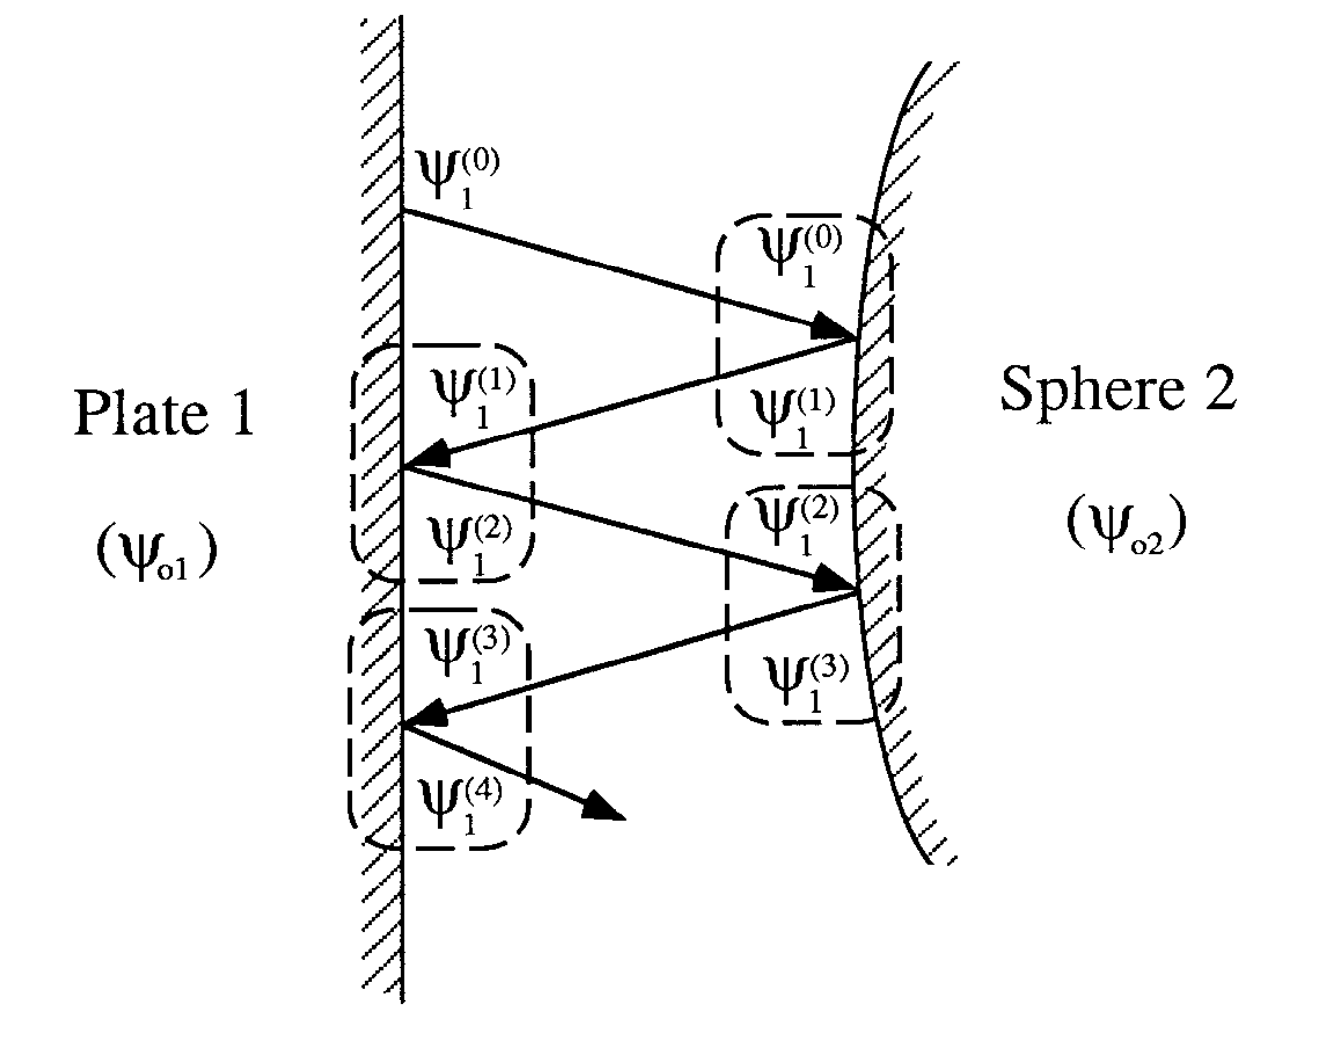
\includegraphics[width=0.45\linewidth,valign=t]{figures/ohshima_corrections_wall.png}
         \textbf{b)}
         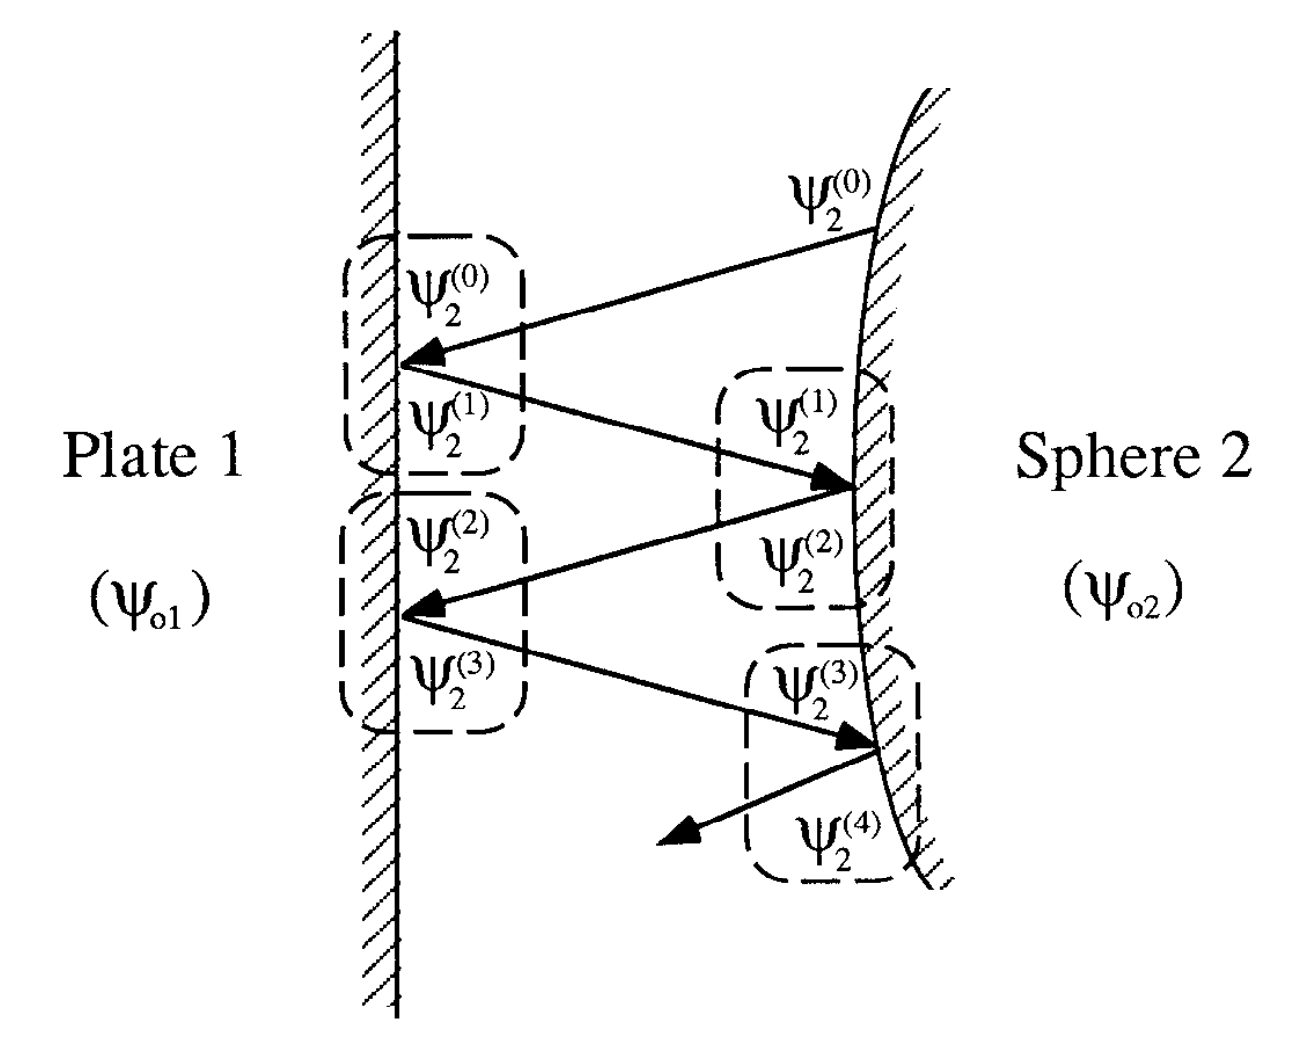
\includegraphics[width=0.45\linewidth,valign=t]{figures/ohshima_corrections_sphere.png}
    \end{minipage}
    \caption{
    \textbf{a)} An order of the wall's electrostatic potential corrections in the approach of Ohshima \cite{ohshima1998}. In this case, an initial potential is the wall's potential $\Psi_1^{(0)}$.  \textbf{b)} Analogously to the left panel, the order of corrections to the sphere's potential $\Psi_2^{(0)}$.
    }
\label{fig:ohshima_corrections}
\end{figure}

Since our system is an interplay of the planar and spherical geometry, all the corrections of the sphere-wall coupled total potential $\Psi$ are based on the various Bessel functions and Legendre polynomials. The explicit formulas are rather complicated and not essential for the scope of this thesis (see Eq. 2.7-29 of Ohshima's work \cite{ohshima1998}). Fig. \ref{fig:ohshima_corrections_compared} compares the subsequent three first steps with each other. The left panel compares the first step $\Psi_{1}^{(1)}+\Psi_{2}^{(1)}$ and the zeroth step $\Psi_{1}^{(0)}+\Psi_{2}^{(0)}$. To see the order of magnitude of the subsequent corrections, we can plot the logarithm of an absolute value of the corrections ratio. Similarly, we can compare the second-order term to the first-order one, depicted in the right panel of Fig. \ref{fig:ohshima_corrections_compared}. For both cases, we see that each correction is much smaller in the sphere's closest vicinity than the previous one. Our main point of interest is the area close to the sphere's surface since this potential affects the sphere's overall force while we seek improvements to our forces model. The first order corrections are at least $10^{3}$ times smaller than the original wall and particle potentials $\Psi_{\textrm{DH,w}}$ and $\Psi_{\textrm{DH,p}}$, and in many regions the potentials ratio is even $\sim10^{-5}$. Even though the logarithm becomes positive in the plot's corners, this is too far away from the surface to affect the overall force on the sphere. The yellow and red regions might emerge because both terms (zeroth and first) are already minimal in such distance from both surfaces, especially for the electrolyte of such a low ionic force as in Ref. \cite{verweij2021}. The terms might vanish at different rates, resulting in such divergent values in the far field. Indeed, the equations of Ref. \cite{ohshima1998} were designed especially for the close proximity region, and we should not bother with the plot's corners.

\begin{figure}
    \begin{minipage}{\linewidth}
         \centering
         \textbf{a)}
         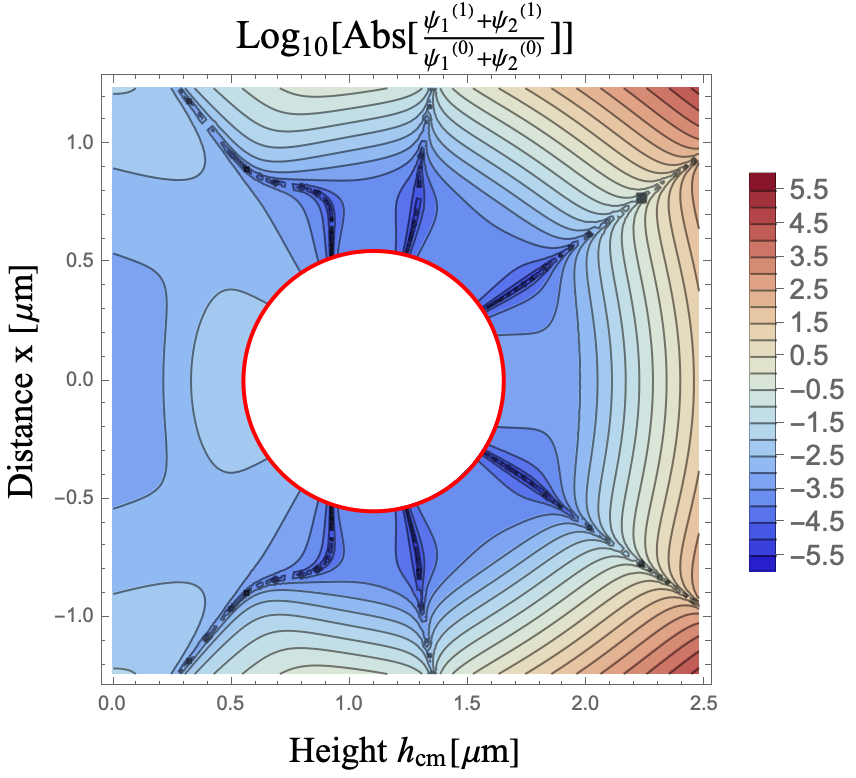
\includegraphics[width=0.45\linewidth,valign=t]{figures/ohshima_first_corrections.png}
         \textbf{b)}
         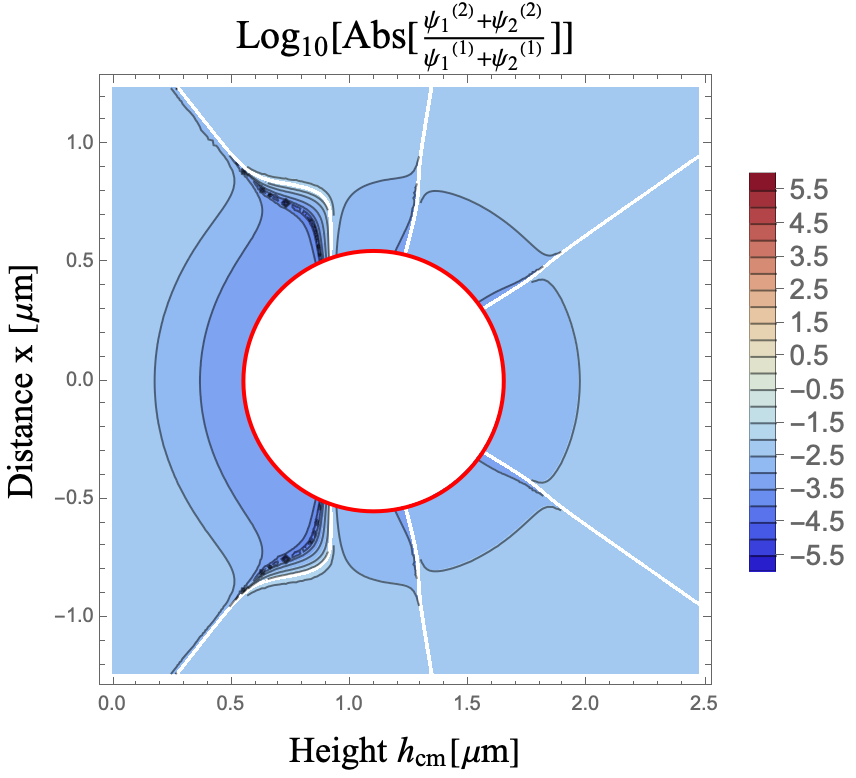
\includegraphics[width=0.45\linewidth,valign=t]{figures/ohshima_second_corrections.png}
    \end{minipage}
    \caption{Comparison between the subsequent electrostatic potential's correction steps in the approach of Ohshima \cite{ohshima1998}. The colours show the logarithm of the absolute value of a ratio between the first and zeroth correction terms (\textbf{a}) and the second and the first correction terms (\textbf{b}). The calculations were conducted for the sphere of radius $a=0.55$ $\mu$m.}
    \label{fig:ohshima_corrections_compared}
\end{figure}

The right panel of Fig. \ref{fig:ohshima_corrections_compared} shows an analogous situation -- the second-term corrections are remarkably smaller than the first ones. Here, the ratio's logarithm is negative for the whole scope of the plot. Therefore, we indeed can claim that the Debye-Hückel approximation and its resultant Eq. \eqref{eqn:electrostatic_force} for $\boldsymbol{F}_{\textrm{el},i}$ can be treated as an accurate generalisation of the Poisson-Boltzmann equation's solution for the case of our system, where we individually treat each sphere's interactions with the wall. Therefore, we should search for some other extensions of our model, such as ones that could explain the preferred-angles phenomenon. Another way to develop the description of electrostatic interactions is to introduce the wall-mediated screening between the dumbbell's spheres. This topic is thoroughly explored in the Section below.


\subsection{Wall's screening} \label{sec:screening}

Since the forces in the original model of Ref. \cite{verweij2021} treat each of the spheres as if they did not interact the second one in any other way than the van der Waals bond, a simple guess would suggest introducing a wall-mediated screening term to our equations. Even though no model in the literature would exactly match our experimental setup of a dumbbell and a wall, few works find the forces on two spheres close to a wall, separated by a given distance. To some extent, we can try to extrapolate these results to the configuration of the joint spheres. This Section will attempt to employ these formulas in our model.

Some clear and elegant expressions for the two separated spheres and a wall were found by Benesch \textit{et al.} \cite{benesch2005}, based on the work of Sader \& Chan \cite{sader_1999}. This approach uses the method of images, where for each sphere of an index $i\in\{1,2\}$, an image sphere of the opposite sign exists at exactly identical distance from the wall on the other side of it. They derive the total force from the wall applied on a single sphere of index $i$, which for the case of identical spheres is given as
\begin{equation}
\begin{split}
    \boldsymbol{F}_{\textrm{s-p-i}} = 4 \pi \varepsilon \kappa a &\Biggl[ \Psi_{\sigma\textrm{,p}} \Psi_{\textrm{eff}} \textrm{exp} \left( -\kappa\left( h_{\textrm{c.m.,}i} - a \right)\right) \\ 
    &+ \Psi_{\textrm{eff}}^2 \biggl[ \left( 1 + \frac{1}{2 \kappa h_{\textrm{c.m.,}i}} \right)\frac{a}{2 h_{\textrm{c.m.,}i}} \textrm{exp}\left(-2\kappa\left( h_{\textrm{c.m.,}i} - a \right)\right) \\ 
    &\qquad\qquad\qquad \left(1 + \frac{1}{\kappa R}\right) \frac{2ah_{\textrm{c.m.,}i}}{R^2} \textrm{exp}\left(-\kappa\left( R - 2a \right) \right) \biggr] \Biggr],
\end{split}
\label{eqn:force_benesch}
\end{equation}
where the first term of Eq. \eqref{eqn:force_benesch} is simply a wall's repulsive force on a sphere (see Eq. \eqref{eqn:edl_potential_wall}. It is scaled by the effective potential $\Psi_{\textrm{eff}}$, given as
\begin{equation}
    \Psi_{\textrm{eff}} = \frac{\Psi_{\sigma\textrm{,p}} - \Psi_{\sigma\textrm{,w}} \Gamma \textrm{exp} (-\kappa h_i)}{1 + \frac{a} {2 h_i \Gamma \textrm{exp} (-\kappa (2 h_i - a))}},
\label{eqn:effective_potential_benesch}
\end{equation}
where the factor $\Gamma$ ensures that the boundary conditions of either constant potential or constant charge on the spheres' surfaces are satisfied. Similarly to the methodology of Ref. \cite{verweij2021}, we can assume the constraint of constant surface potential and therefore $\Gamma = \textrm{sinh}(\kappa a) / \kappa a$. The second term of Eq. \eqref{eqn:force_benesch} acquires for the repulsion from the image of the original sphere, and the last term originates from the second sphere's image.  The length scales of Eq. \eqref{eqn:force_benesch} and \eqref{eqn:effective_potential_benesch} are the distance $h_i$ between the centre of sphere $i$ and the wall, and $R$, which is the distance between centres of the original sphere and an image of the second sphere. Besides the wall's repulsion on the sphere, the original paper of Ref. \cite{benesch2005} also expresses the sphere-sphere repulsion. However, in our case, we can assume it to be entirely suppressed by the strong van der Waals attraction that bonds the dumbbell particle.

Having the new forces model defined, we can examine its dependency on the dumbbell's separation $h_{\textrm{c.m.}}$ and orientation $\theta$. The left panel of Fig. \ref{fig:walls_screening} shows how the new total force on a dumbbell, given as $F_{\textrm{scr}}=|\boldsymbol{F}_{\textrm{g},1}+\boldsymbol{F}_{\textrm{g,}2}+\boldsymbol{F}_{\textrm{s-p-}1}+\boldsymbol{F}_{\textrm{s-p-}2}|$, depends on ($h_{\textrm{c.m.}}$, $\theta$) for the sphere size $a=0.55$ $\mu$m. The model parameters, like $\Psi_\textrm{p}$, $\kappa^{-1}$ etc., are exactly the same as for Fig. \ref{fig:small_dumbbells_simulation_distributions}. First of all, we see that the particle's optimal height grows with $\theta$, similar to the results of Ref. \cite{verweij2021}. However, the values of $h_{\textrm{c.m.}}(F_{\textrm{scr}}\simeq0)$ are noticeably larger than the ones of Fig. \ref{fig:force_torque_distributions}, and larger than the most common ones in the experiment results. It can be surprising that while the theory of Ref. \cite{verweij2021} does not take the wall's screening into account, it seems that it predicts $p(h_{\textrm{c.m.}})$ better than its screening-including extension. However, we need to remember the arbitrariness of the choice of $\kappa^{-1}$. Since the different values of Debye length can change the total potential significantly, there is a chance that if we calculate new probability densities that include $F_{\textrm{scr}}$ and then fit them to the data, we would again obtain a satisfactory fit. However, instead of simple fitting of another distribution to the data, let us first analyse the new torque on our particle.

The right panel of Fig. \ref{fig:walls_screening} shows how the new total torque $\boldsymbol{T}_{\textrm{scr}}$, that results from the approach of Benesch \textit{et al.}, depends on ($h_{\textrm{c.m.}}$,$\theta$). The plot is antisymmetric with respect to wall-parallel $\theta=0$, as it already was for our basic model. The signs in both halves of the plot suggest that the new torque still drives the dumbbell to the ideally parallel orientation. Therefore, the simple model of the second sphere's screening does not cause twisting force on the dumbbell, which we are trying to understand in this thesis.

\begin{figure}
    \centering
    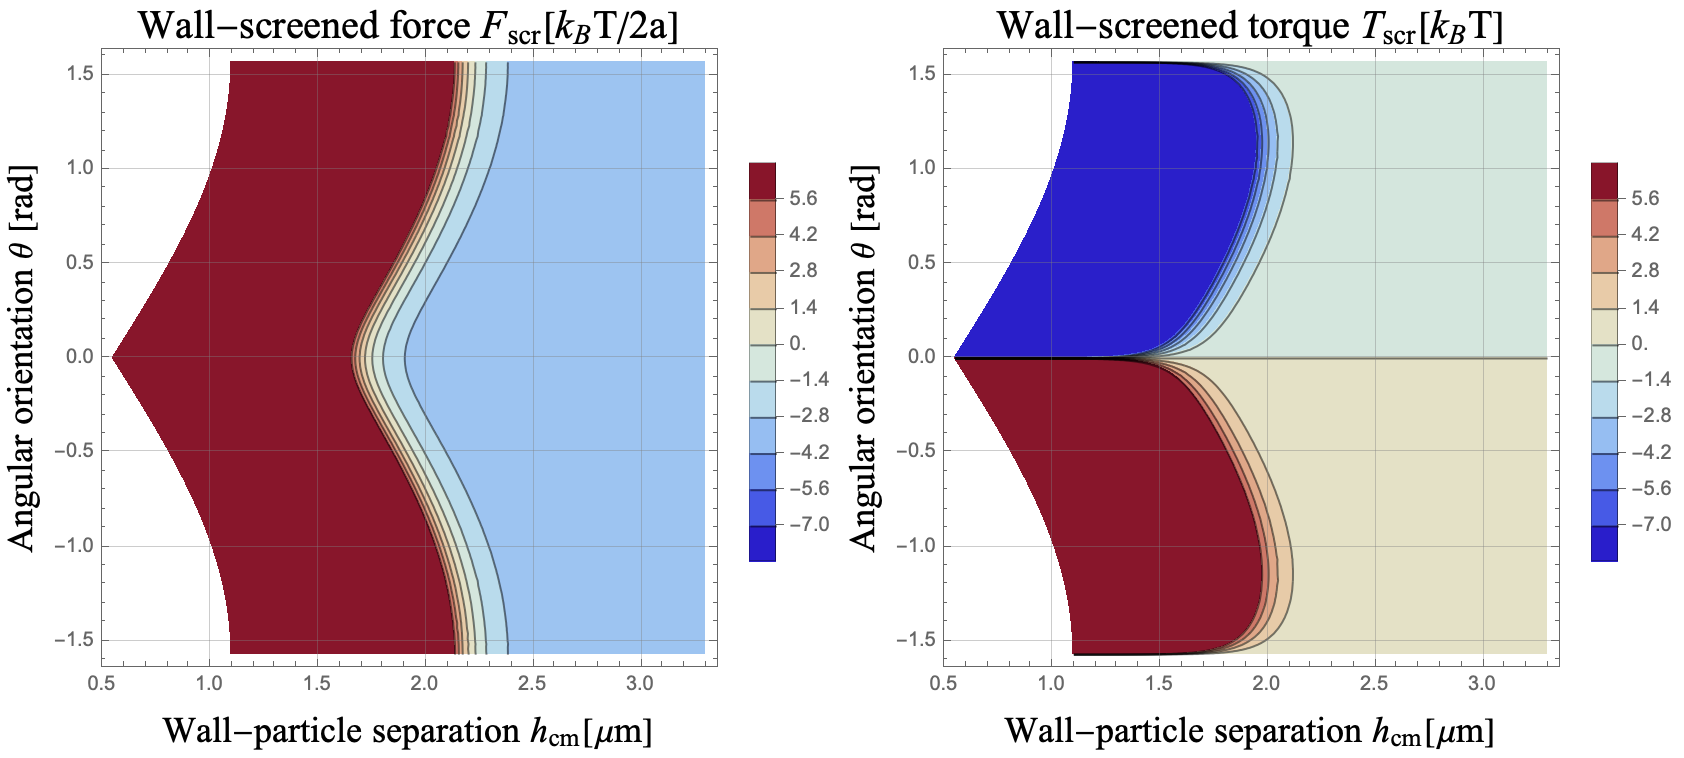
\includegraphics[width=\linewidth]{figures/walls_screening.png}
    \caption{\textbf{Left:} Wall-screened force $F_{\textrm{scr}}$ on a dumbbell particle with the second-sphere-screening term (see Eq. \eqref{eqn:force_benesch}) included in the equations. \textbf{Right:} Wall-screened torque $T_{\textrm{scr}}$ for the dumbbells of the force model extended with the approach of Benesch \textit{et al.} \cite{benesch2005}.}
    \label{fig:walls_screening}
\end{figure}

Even though the model of Benesch \textit{et al.} provides the screening terms for both spheres, it cannot explain the observations of the preferred angles in the experiment of Ref. \cite{verweij2021}. It might be possible to obtain satisfactory probability densities of $h_{\textrm{c.m.}}$ with the screening model. However, due to the lack of potential in finding the twisting force, we should try to consider other unexplored phenomena and not focus on modifying the Eq. \eqref{eqn:dumbbell_height_distribution}. The similar screening models of Qian \& Bowen \cite{qian1999} and some other approaches developed especially for this research could also not reproduce the twisting effect.

It is important to note that the models mentioned above are still relatively simple and often designed for the separated sphere case. They still do not consider the shapes (or their superpositions) of EDL other than the planar and spherical ones (see Eq. \eqref{eqn:edl_potential_wall} and \eqref{eqn:edl_potential_sphere}). We could try to study some more complex shapes numerically, for example, with the finite elements method (FEM). However, this is a relatively difficult task beyond the scope of the research presented here. While numerical FEM-based solutions are discussed in Section \ref{sec:other_hypotheses}, let's first inspect the assumptions on the shperes' surface potentials.

\subsection{Surface potentials}

Another simplification included in the model of Ref. \cite{verweij2021} is the assumption of constant Stern potential values at the surfaces of both dumbbell spheres. However, in real-life situations, it is likely that the values of $\Psi_{\textrm{S}}$ for each sphere are at least slightly different. Therefore, we can introduce a coefficient $\alpha$ as a measure of the disproportion between both spheres' potentials. The scaled electrostatic force $\boldsymbol{F}_{\textrm{el,}\alpha}(h_{\textrm{c.m.}})$ would then become
\begin{equation}
    \boldsymbol{F}_{\textrm{el,}\alpha}(h_{\textrm{c.m.}}) = 64 \pi \varepsilon \kappa a \left( \frac{k_B T}{e} \right)^2 \textrm{tanh} \left( \frac{e \Psi_w}{4 k_B T} \right) \textrm{tanh} \left( \frac{e \alpha \Psi_p}{4 k_B T} \right) \textrm{exp} \left(- \kappa h_{\textrm{c.m}.,i} \right) \hat{\boldsymbol{n}},
\label{eqn:scaled_electrostatic_force}
\end{equation}
and the total force would be $\boldsymbol{F}_{\alpha}=2\boldsymbol{F}_{\textrm{g}} + \boldsymbol{F}_{\textrm{el,}1} + \boldsymbol{F}_{\textrm{el,}\alpha}$, where $\boldsymbol{F}_{\textrm{el,}1}$ is the force on the sphere of an unchanged potential. For now, let's assume the scaled surface potential $\alpha \Psi_{\textrm{p}}$ to be smaller than the original one and, therefore, $\alpha \in (0, 1\rangle$. An example plot of $F_{\alpha}(h_{\textrm{c.m.}, \theta})=|\boldsymbol{F}_{\alpha}(h_{\textrm{c.m.}, \theta})|$ is presented in the left panel of Fig. \ref{fig:different_sterns_force_torque}. The calculations were conducted for $\alpha=0.01$, which is a striking disproportion. However, we see that for such an extreme case, the isoline of zero force is indeed shifted towards non-zero $\theta$. For comparison, the violet dot symbolises the most common experimentally observed configuration ($h_{\textrm{c.m.}}=1.30$ $\mu$m, $\theta \simeq 0.56$ rad). For this value of $\theta$, the black point is clearly higher than the one of $F_{\textrm{el,}\alpha}=0$. Therefore, although introducing a simple potential disproportion might be a clue in our considerations, it is not enough to fully reproduce the observed phenomenon.

\begin{figure}
    \centering
    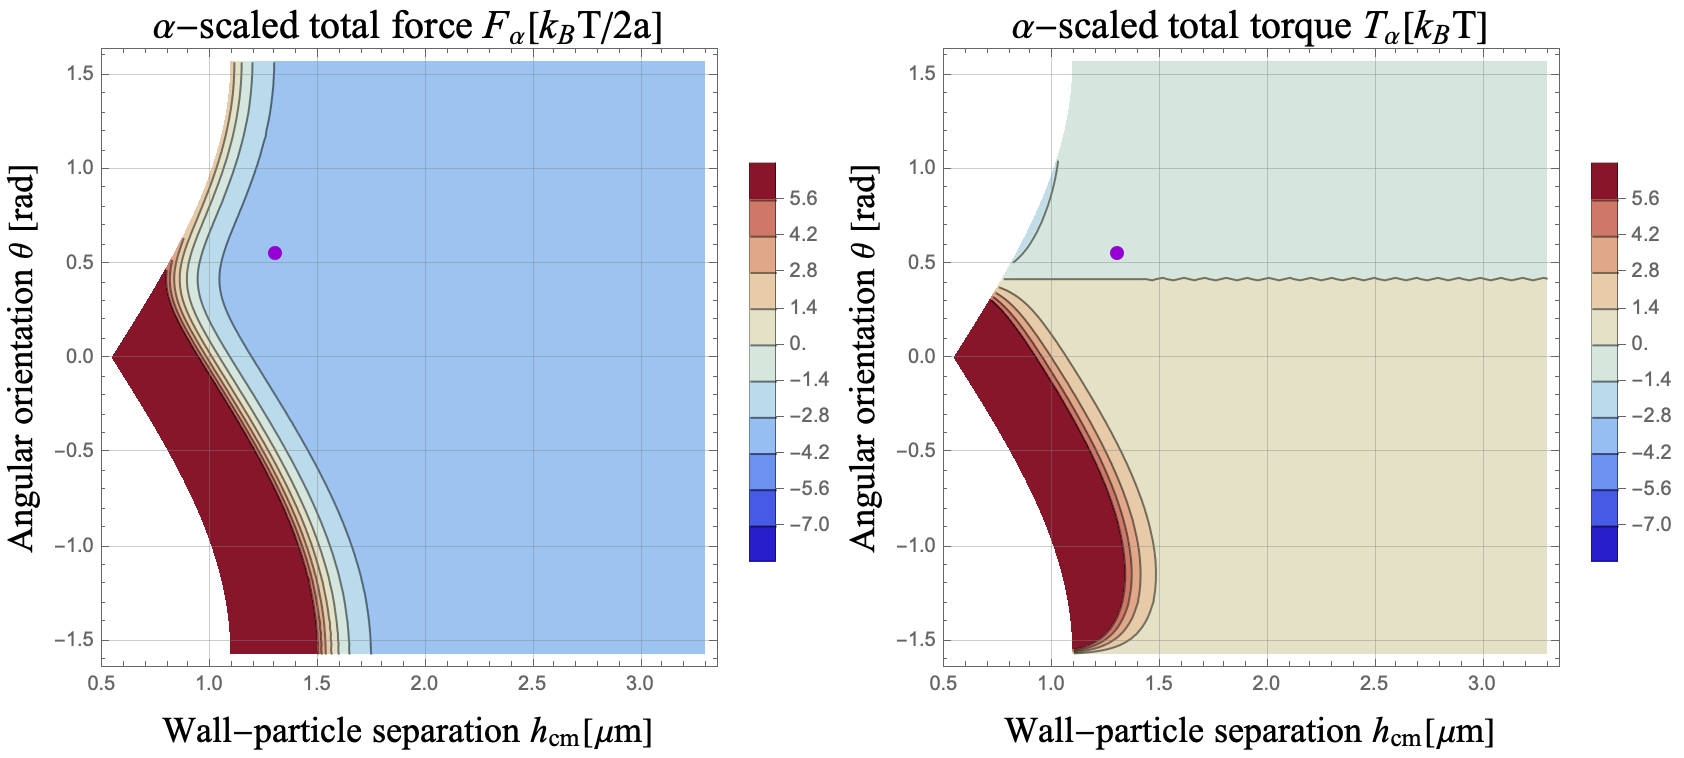
\includegraphics[width=\linewidth]{figures/different_sterns_force_torque.png}
    \caption{\textbf{Left:} Total force on a dumbbell $F_{\alpha}$ for the $\alpha$-scaled forces model (see Eq. \eqref{eqn:scaled_electrostatic_force}). Violet dot symbolises the most common experimentally-observed configuration of wall-particle separation $h_{\textrm{c.m.}}=1.30$ $\mu$m and orientation $\theta=32^{\circ}\simeq 0.56$ rad. The white regions are the geometrically restricted configurations. \textbf{Right:} Analogous plot for the $\alpha$-scaled torque $T_{\alpha}$.}
    \label{fig:different_sterns_force_torque}
\end{figure}

The right panel of Fig. \ref{fig:different_sterns_force_torque} shows how the resultant total torque $T_{\alpha}=|\boldsymbol{T}_{\alpha}|$ depends on the particle's ($h_{\textrm{c.m.}}$,$\theta$) when $\alpha=0.01$. Here, the isoline of zero torque is horizontal, which means that the torque balance is independent of $h_{\textrm{c.m.}}$, and there is only one value of $\theta$ where the particle is rotationally stable.  Similarly to the right panel of Fig. \ref{fig:walls_screening}, the plot is divided into two parts, with negative torque in the upper part and positive in the lower part. As we focus on the upper part of both Fig. \ref{fig:walls_screening} plots, we see that the regions of low repulsive force and low negative torque (comparable with the thermal fluctuations energy) are relatively close to the wall's boundary. Some isolines are even covered by the white region of the geometrically forbidden configurations. Therefore, it is worth considering a model's extension that would include some short-range interactions like the Lennard-Jones potential or simply the hard-core interactions that would forbid the possible intersection of a wall.

The drift term drives the dumbbells to some specific orientation and tries to preserve it. However, the presence of Brownian motion expands the probability distributions $p(h_{\textrm{c.m.}})$ and $p(\theta)$, previously described with Eq. \eqref{eqn:dumbbell_height_distribution} and \eqref{eqn:dumbbell_orientation_distribution}. For the dissimilar Stern potentials analysis, we need to introduce a modified version of dumbbell's potential energy $\phi(h_{\textrm{c.m.}}, \theta)$, previously described with Eq. \eqref{eqn:dumbbell_potential_energy}. The new formula for $\phi_\alpha(h_{\textrm{c.m.}}, \theta)$ is given as
\begin{equation}
    \phi_\alpha(h_{\textrm{c.m.}}, \theta) = -2 F_\textrm{g} h_{\textrm{c.m.}} + \frac{ F_{\textrm{el},i}(h_{\textrm{c.m.}})}{\kappa} \textrm{exp}\left( -\kappa a \textrm{sin}(\theta) \right) + \frac{ F_{\textrm{el,}\alpha}(h_{\textrm{c.m.}})}{\kappa} \textrm{exp}\left( \kappa a \textrm{sin}(\theta) \right),
\label{eqn:scaled_dumbbell_potential_energy}
\end{equation}
Then, the new probability distributions $p_\alpha(h_{\textrm{c.m.}})$ and $p_\alpha(\theta)$ can be calculated through integration of $\phi_\alpha(h_{\textrm{c.m.}}, \theta)$ with respect to one of the variables. These scaled probabilities are presented as the black curves in Fig. \ref{fig:different_sterns_simulation}. The left panel shows the height distribution, whereas in the right one, there are dumbbells' angular orientations. The cyan histograms represent the numerical simulation outcomes for the same algorithm as in Section \ref{sec:wall_results}, with the changed formula for the electrostatic force on one of the spheres.

As we see, in both of the Fig. \ref{fig:different_sterns_simulation} panels, the agreement between the simulation and black lines of $p_\alpha(h_{\textrm{c.m.}})$ and $p_\alpha(\theta)$ is relatively good. However, we can see certain disparities compared to our previous analysis of Fig. \ref{fig:different_sterns_force_torque}. First of all, the maximum of heights probability distribution $p_\alpha(h_{\textrm{c.m.}})$ is at $\sim 1.30$ $\mu$m, whereas the point of $F_{\alpha}=T_{\alpha}=0$ is at less than $1.00$ $\mu$m. The difference between these heights is due to the significantly larger gradient of $\phi_{\alpha}(h_{\textrm{c.m.}},\theta)$ in the wall's proximity. While dumbbell sedimentation is a relatively peaceful process with constant acceleration $g$, the electrostatic repulsion can be very rapid, especially when the Brownian motion drives the particle significantly close to the interface. In other words, even though the particle tends to the point of zero force, the distribution is strongly limited and pushed away from the wall's side. In contrast, the other side's moderate potential gradient makes the diffusion less suppressed.

When we look at the right panel of Fig. \ref{fig:different_sterns_simulation}, we see a distribution shift towards a certain angle, relatively close to the most common angle of $32^{\circ}$. However, we still obtain many configurations of the orientations close to wall-parallel $0^{\circ}$. This is contrary to the measurements of Ref. \cite{verweij2021}, depicted with the violet curve, where none of such configurations were observed. Moreover, the simulated distribution has one maximum, whereas the experimental results form a double-peaked structure. There is no possibility that simple scaling of one of the dumbbell's Stern potentials would separate the $p_{\alpha}(\theta)$ distribution into two regions. Therefore, this simple approach is not enough to truly reproduce the experimental distributions.

It is worth mentioning that the $\alpha$-modified simulations model, results of which are presented in Fig. \ref{fig:different_sterns_simulation}, experienced slight particle intersections into the wall's body. However, the preliminary results show different behaviours from the experimentally observed one, and the short-range interactions would even enhance wall-parallel reorientation. Since the motivation of this thesis is to find the source of preferred non-parallel orientations, no specific developments were applied to the case of the wall-penetrating particles.

\begin{figure}
    \centering
    \includesvg[width=\linewidth]{figures/different_sterns_simulation.svg}
    \caption{Numerical simulation results (cyan histograms) for the system of $10^5$ dumbbell particles with the $\alpha$-scaled surface potential on one of the spheres. The histograms were calculated for the simulation's last timestep, namely $t = 30$ s. The black lines are analytical expressions for $p_{\alpha}(h_{\textrm{c.m.}})$ (left panel) and $p_{\alpha}(\theta)$ (right panel). The violet line symbolises the experimental histogram of Ref. \cite{verweij2021} obtained for the particles of sphere radius $a=0.55$ $\mu$m.}
    \label{fig:different_sterns_simulation}
\end{figure}

At first, it might be surprising that for such a dramatic change of one sphere's potential ($\alpha=0.01$), the equilibrium point is still relatively similar to that of $\alpha=1$. However, when we return to Eq. \eqref{eqn:scaled_electrostatic_force}, we notice that, in fact, there are two terms that change in this expression. The first one is the potential $\alpha\Psi_{\textrm{p}}$, that we change intentionally. Due to this modification, for the case of $\alpha\in (0,1\rangle$, the scaled-potential sphere receives less repulsion from the wall and the equilibrium between $\boldsymbol{F}_{\textrm{g}}$ and $\boldsymbol{F}_{\textrm{el},\alpha}$ shifts to the lower values of $h_{\textrm{c.m.}}$. Therefore, the exponential term in Eq. \eqref{eqn:scaled_electrostatic_force} also changes. The exponential function grows more rapidly as the $h_{\textrm{c.m.},i}$ decreases (see Fig. \ref{fig:influence_of_kappa}) in comparison with the $\textrm{tanh}$ of the scaled potential. This is why the coefficient $\alpha$ needs to be so low to allow the less-charged sphere to achieve such close proximity to the wall, even though the relative change of $h_{\textrm{c.m.}}$ is not so significant.

In this Section, our calculations have already shown that the potential disproportion can indeed result in some kind of a dumbbell-twisting effect. However, the new distributions do not seem to capture the whole phenomenon observed in Ref. \cite{verweij2021}. To make sure whether we can at least obtain the distributions for which their maxima coincide with the point of most-common $h_{\textrm{c.m.}}=1.30$ $\mu$m and $\theta=0.56$ rad (black point in Fig. \ref{fig:different_sterns_force_torque}), we can numerically find these maxima, namely $\textrm{max}(p_\alpha(h_{\textrm{c.m.}}))$ and $\textrm{max}(p_\alpha(\theta))$, for certain chosen values of $\alpha\in\{ 0.01, 0.1, 0.2, \dots, 0.9, 1 \}$. They are represented with the green dots in the left panel of Fig. \ref{fig:different_sterns_max_and_ratio}. For the relatively similar values of potentials, the dots are relatively close, and the dumbbell remains rather wall-parallel than twisted. However, when the disproportions get more prominent, the points of maximum become more separated. However, the dashed green line connecting the point for $\alpha=1$ and $\alpha=0.01$ clearly does not coincide with the violet point of the experimental results. We see that it is impossible to reproduce the experimental distributions with simple manipulations of $\alpha$. However, this is not the only way to manoeuvre the system's parameters.

While we have analysed the $\alpha\in (0, 1\rangle$ case, we might wonder what would happen for the case of $\alpha>1$. This would lead us to a configuration where the scaled-potential sphere tends to be at higher separations than the one of unchanged $\Psi_{\textrm{p}}$. However, the exponential nature of the EDL repulsion is crucial in this scenario as well. While large disproportion of $\alpha \ll 1$ can cause the dumbbell to rotate, the magnitude of $F_{\textrm{el},\alpha}$ decays so fast that the scaled-potential sphere stays at nearly the same heights for even large values of $\alpha \gg 1$. In other words, for the values of $\alpha>1$, the red points of Fig. \ref{fig:different_sterns_max_and_ratio} left panel would not change their locations to a noticeable extent.

Until now, we have been only changing the Stern potential of one of the dumbbell's spheres. A different approach is changing both values of $\Psi_\textrm{p}$ values to obtain a specific torque. To investigate this, we can look at the right panel of Fig. \ref{fig:different_sterns_max_and_ratio}. It shows the total torque calculated for two modifiable Stern potentials -- $\Psi_{\textrm{L}}$ on the lower sphere  and $\Psi_{\textrm{U}}$ on the upper one. While the force Equations \eqref{eqn:electrostatic_force} and \eqref{eqn:scaled_electrostatic_force} are using the Stern potentials explicitly, the authors of Ref. \cite{verweij2021} are fitting values of the $\zeta$-potential $\Psi_{\zeta}$ to the experimental data. Therefore, the axes of Fig. \ref{fig:different_sterns_max_and_ratio} right panel are adjusted to $\Psi_{\zeta,\textrm{L}}$ and $\Psi_{\zeta,\textrm{U}}$. In fact, the connection between the scaling of the Stern potentials and the $\zeta$-potentials is linear. Nonetheless, looking at the plot, we see that the torque nearly completely does not depend on the absolute value of $\Psi_{\zeta,\textrm{U}}$; it is only the case of $\Psi_{\zeta,\textrm{L}}$ or the ratio between the potentials. The plot's isolines for two different potential values are predominantly vertical. Therefore, we can exclude the approach of changing both $\Psi_{\textrm{L}}$ and $\Psi_{\textrm{U}}$ and focus on some other system's parameters.

\begin{figure}
    \centering
    \includegraphics[width=\linewidth]{figures/different_sterns_max_and_ratio.png}
    \caption{\textbf{Left:} Points of maxima of $p(h_{\textrm{c.m.}},\theta)$ for various coefficients of Stern potentials disproportion $\alpha$ (green dots), with the points of $\alpha=0.01$ and $\alpha=1$ joined with the green dashed line. The violet dot symbolises the most common configuration observed in Ref. \cite{verweij2021}, equal to $h_{\textrm{c.m.}}=1.30$ $\mu$m and $\theta=0.56$ rad. \textbf{Right:} Total torque on a dumbbell with two different $\zeta$-potentials on the lower $\Psi_{\zeta,\textrm{L}}$ and upper $\Psi_{\zeta,\textrm{U}}$ sphere. The violet dot represents the configuration of the equal potential $\Psi_{\zeta\textrm{,p}} = -0.03$ V, as fitted in Ref. \cite{verweij2021}.}
    \label{fig:different_sterns_max_and_ratio}
\end{figure}

The Stern potential is related to $\kappa^{-1}$, especially in the methodology of Verweij \textit{et al.} \cite{verweij2021}, where the authors were fitting both of these parameters, determining their initial values based on the Eq. \eqref{eqn:edl_potential_sphere}. This suggests that when we change one sphere's potential, we might also need to change its corresponding Debye length. A slightly simpler idea is to investigate how the probability distributions change with $\alpha$ and $\kappa^{-1}$ based on a few example calculations of the distributions $p_{\alpha}(h_{\textrm{c.m.}})$ and $p_{\alpha}(\theta)$ for various values of $\kappa^{-1}$. Fig. \ref{fig:different_sterns_and_kappas} shows how the scaled probabilities $p_{\alpha}(h_{\textrm{c.m.}})$ (top panels) and $p_\alpha(\theta)$ (bottom) change with different values of $\kappa^{-1}$ (left) and $\alpha$ (right). We see that for the relatively small $\kappa^{-1}=103$ nm, the potential disproportion does not largely influence the heights at which the dumbbells float. For example, for the relatively large potentials disparity $\alpha=0.01$, the distribution's shift is actually less than $0.5$ $\mu$m in comparison with the $\alpha=1$ curve. Conversely, the choice of $\kappa^{-1}$ strongly changes $p_{\alpha}(h_{\textrm{c.m.}})$. The brown and dashed black curve in the top right panel are plotted for the same $\kappa^{-1}$ but for different $\alpha$, namely equal to $1$ (black) and $0.1$ (brown). While the difference between them is not significant, the Debye length value change makes dumbbells float much higher above the wall. The green line represents a configuration where the value of the Debye length $\kappa^{-1}$ is the same as for larger dumbbells. Indeed, the distribution resembles the one of Fig. \ref{fig:dumbbell_shortcomings} right panel, even though it was calculated for the smaller particles. Once again, we see that the choice of $\kappa^{-1}$ is the most important out of all parameter fittings performed by Verweij \textit{et al.} \cite{verweij2021}.

When it comes to angular distributions $p(\theta)$ (bottom panels of Fig. \ref{fig:different_sterns_and_kappas}), we see that the change of $\alpha$ has more impact on the strength of the dumbbell-twisting effect than $\kappa^{-1}$. In fact, we introduced the scaling factor to force our dumbbells to change their orientations. As shown in Fig. \ref{fig:different_sterns_max_and_ratio}, the dumbbells remain wall-parallel for the relatively similar sphere potentials. However, it changes in the case of significant disparities. However, as we see in the bottom right panel, for the spheres of different potentials ($\alpha=0.1$), the larger values of $\kappa^{-1}$ can shift $p(\theta)$ towards the larger angles as well. Obviously, this does not happen for the case of $\alpha=1$, where both spheres are repelled by the wall with the same force, and the distribution is always centred at $\theta=0$.

\begin{figure}[h]
    \centering
    \includesvg[width=\linewidth]{figures/different_sterns_and_kappas.svg}
    \caption{Probability densities for the $\alpha$-scaled forces model on a dumbbell particle, for various values of $\kappa^{-1}$ and $\alpha$. Top panles show the height distributions $p_{\alpha}(h_{\textrm{c.m.}})$, whereas the bottom ones present the angular orientation distributions $p_{\alpha}(\theta)$. The black lines represent the original fits of Ref. \cite{verweij2021} to the data gathered for the smaller dumbbells of $a=0.55$ $\mu$m. The violet curves represent the $\theta$-histogram for the smaller dumbbell measurements. All the curves are normalised by their maximum value.}
    \label{fig:different_sterns_and_kappas}
\end{figure}

The violet histograms in the bottom panels of Fig. \ref{fig:different_sterns_and_kappas} represent the experimental results of Ref. \cite{verweij2021}. Whereas the maximum values of angular distributions seem to coincide for very large potential disproportions and the largest $\kappa^{-1}$ of the ones considered in Ref. \cite{verweij2021}, the wall-parallel configurations are still largely present. For the smaller dumbbells of single sphere radius $a=0.55$ $\mu$m, these orientations were unobserved. Moreover, there is still no phenomenon that would result in the double-peaked probability curve. This suggests that while we could modify specific system parameters to make dumbbells tilt, the nature of the original phenomenon seems to be different. The torque that we search for maintains the particle in the preferred position with the magnitude of at least few $k_{\textrm{B}}T$ (see Fig. \ref{fig:force_torque_distributions}), which is unachievable with the methods we have considered for now. 

In this section, we have shown that various manipulations of $\Psi_{\textrm{L}}$, $\Psi_{\textrm{U}}$ and $\kappa^{-1}$ can indeed cause the dumbbells to orient at some preferred angles. It is possible that another degree of freedom, namely two possible values of $\kappa^{-1}$ for each sphere, would bring us even closer to the experimental distributions. However, this approach does not capture the whole nature of the phenomenon we search for. Moreover, the potential disparity of the order $\alpha=0.01$ seems unrealistic and probably impossible to achieve in the aforementioned experimental setup. Therefore, we should explore some phenomena of a different nature rather than the EDL distortion alone. One such is a geometrical dissimilarity between the spheres, already analysed by the authors of Ref. \cite{verweij2021}.


\subsection{Polysized dumbbells}

Another simple guess of the potential reason for the disparity between our theoretical model and the experimental results is the idea that the spheres of a dumbbell could be of different sizes, for example, due to the inhomogeneities in the manufacturing process. Intuitively, this would indeed shift the minimum energy configuration to $\theta \neq 0^{\circ}$. The authors of Ref. \cite{verweij2021} have performed such an analysis themselves in a supplementary Section V of their work. In this Section, we will examine their analysis.

By modifications of $p(h_{\textrm{c.m.}},\theta)$, the authors find a new expression for the probability distribution $p(a_1,a_2)$ of the polysized dumbbells of sphere radii $a_1$ and $a_2$ (see Eq. 11 and Eq. 14-20 in Ref. \cite{verweij2021}). They plot it for the case of $5\%$-difference in the sphere radii, which could be possible due to possible inaccuracies in the colloidal spheres production process. The $ 5\%$ difference also corresponds to the potential error in the particle size measurements. While there is nearly no change in the probability distribution for this case compared to the equally-sized spheres, interesting observations emerge for the extreme cases where one sphere is approximately twice the size of a second one. Fig. \ref{fig:polysized_distributions} shows other plots of Ref. \cite{verweij2021}, where authors calculate $p(a_1, a_2)$ for the sphere sizes $a_1=0.33$ $\mu$m, $a_2=0.65$ $\mu$m (left panel) and for the larger $a_1=0.63$ $\mu$m, $a_2=1.26$ $\mu$m (right panel). While none of these radii is equal to $0.55$ $\mu$m nor $1.05$ $\mu$m, which were used in the experiment, the overall particle volumes are equal to the ones of the setup. Therefore, the gravity force acting on a smaller and larger polysized dumbbell is the same as for the smaller and larger unisized ones. The only force that changes in this model is the electrostatic repulsion.

\begin{figure}
    \centering
    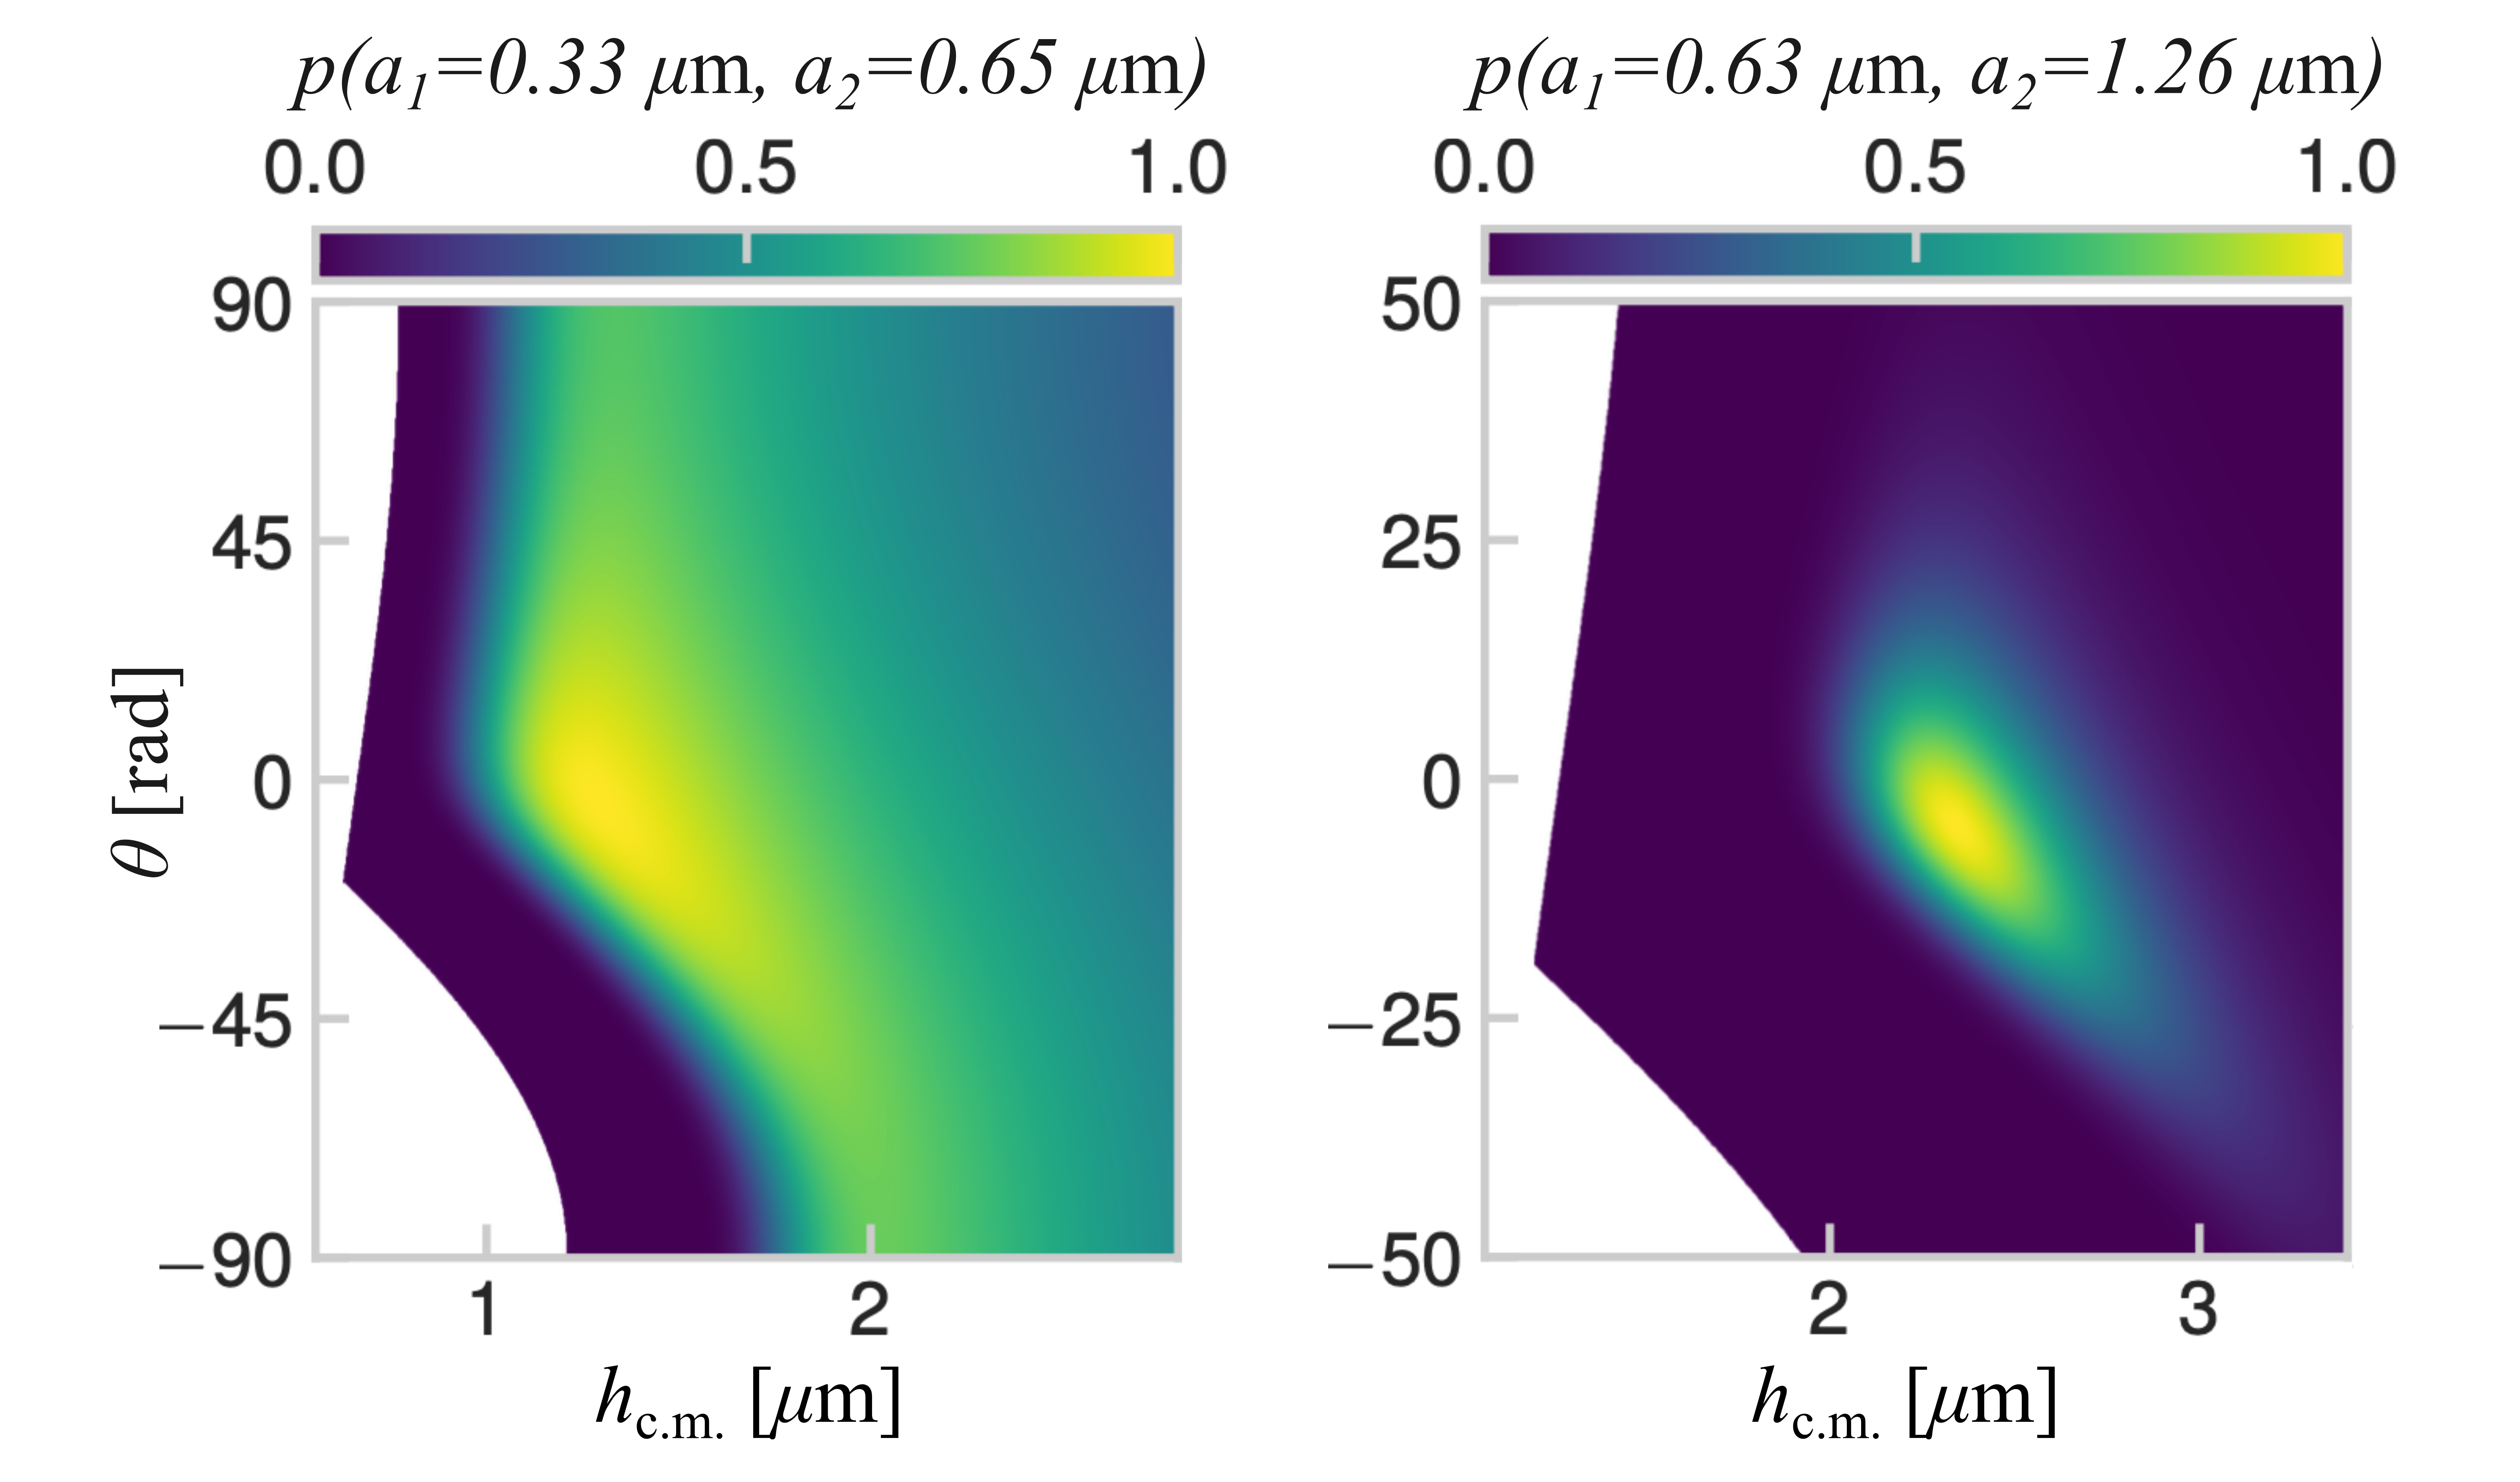
\includegraphics[width=0.8\textwidth]{figures/polysized.png}
    \caption{Probability distributions $p(a_1,a_2)$ for the polysized dumbbells of the single sphere radii $a_1=0.33$ $\mu$m, $a_2=0.65$ $\mu$m (left) and $a_1=0.63$ $\mu$m, $a_2=1.26$ $\mu$m (right). The results were obtained using Eq. 14-20 from Ref. \cite{verweij2021}. Attribution: Verweij \textit{et al.} \cite{verweij2021} (Fig 6j and 7j). These plots are directly reproduced from the original source.}
\label{fig:polysized_distributions}
\end{figure}

Looking at the smaller polysized dumbbell distribution, we see that even such a large disparity in sphere sizes does not bring us close to the experiment results. Even though $p(a_1,a_2)$ became asymmetrical, the distribution maximum is still relatively close to $\theta=0^{\circ}$. The ideally-parallel configurations are still highly probable, contrary to the complete lack of such in the observations. However, the results of larger polysized dumbbells (right panel) are more similar to those of the experimental ones. The median measured orientation for a sphere radius $a=1.05$ $\mu$m was $6^{\circ}$, which resembles the right panel plot. However, the most frequently observed separation was $h_{\textrm{c.m.}}\simeq2.0$ $\mu$m. For the polysized dumbbell, nearly whole $p(0.63\textrm{ }\mu \textrm{m},1.26\textrm{ }\mu \textrm{m})$ is above $2$ $\mu$m. Moreover, the probabilities are again single-peaked, whereas the experimental outcomes form the two-peaked structures.

The analysis of Verweij \textit{et al.} \cite{verweij2021} shows that the potential disparities in sphere sizes could shift the probability distributions towards non-zero values of $\theta$. However, the disproportion would need to be so large that the authors would actually need to connect smaller spheres with the larger ones in each dumbbell particle. Therefore, while we again see that various dissimilarities between the spheres can seem to bring us closer to the experimental results, they are too weak to be the primary cause of the dumbbell-twisting phenomenon.


\subsection{Other hypotheses and comparison} \label{sec:other_hypotheses}

While various dissimilarities between the dumbbell's spheres can induce some kind of reorientation to the preferred angles, they do not reproduce the observation of lack of wall-parallel orientations of the smaller particles nor the double-peaked distribution structures. In the following paragraphs, we will discuss a few other hypotheses that could explain the surprising dumbbell-twisting behaviour and, in the end, summarise all our efforts of this long Section.

According to the observations of Zöttl \textit{et al.} \cite{zottl_2019}, the shear channel flow can make the rod-like Brownian particles rotate and maintain non-parallel orientations. In particular, it is possible for the particle to perform the 'kayaking' motion, which is the authors' name for the paddling-resembling movement of the rod. In fact, it is possible that the experiment of Verweij \textit{et al.} \cite{verweij2021} was not free from, i.e. spontaneous convection that would influence the dumbbell behaviour. However, the 'kayaking' pattern contains also the configurations of $\theta=0^{\circ}$, unobserved for the particles of $a=0.55$ $\mu$m. Moreover, it would be even more surprising if the uncontrolled convection would not cause any single dumbbell to orient parallel to the wall. Finally, the shear rate applied in Ref. \cite{zottl_2019} is $\dot{\gamma}=18$ s$^{-1}$, which was surely impossible to achieve in our system. The possible uncontrolled flows in the experimental sample holder of Ref. \cite{verweij2021} do not seem to explain the preferred-angles phenomenon.

To investigate the short-range interactions between the colloidal particles and the walls, one can apply the Lennard-Jones potential $\Psi_{\textrm{LJ}}$ (see Eq. \eqref{eqn:lennard_jones}) to the simulations, as in the work of Lambert \textit{et al.} \cite{lambert_2024}. As mentioned in Section \ref{sec:electr_theory}, the length scales of $\Psi_{\textrm{LJ}}$ are significantly smaller than $\kappa^{-1}$. However, an interesting observation is that if we set $\sigma$ as equal to the Debye length and replace the electrostatic potential in our model $\Psi_{\textrm{el}}$ with $\Psi_{\textrm{LJ}}$, we can still achieve very similar results. While it cannot be connected to any real-life system, the shape of our potential can be less important in our computations than one could have expected.

Another guess about the reason for the preferred-angles observation is the polarisation of the dumbbell particle. Since the particle is made of dielectric material, it can get polarised in the presence of the electric field of the wall's EDL. Since the polarised material tends to maintain its state, a strong polarisation could be the only phenomenon considered here to sufficiently preserve the preferred angular orientation and prevent the smaller dumbbells from reaching the wall-parallel configurations. Moreover, the lower electrostatic potential at larger separations characteristic for the larger dumbbells would cause less significant polarisation, which aligns with the observations for $a=1.05$ $\mu$m. The larger dumbbells were also obtained from a different source than the smaller ones. The differences in the manufacturing process could also influence the polarisation patterns.

However, even if the polarisation explains the strong maintenance of specific angles, there is still a question why these particular angles are preferred. In previous sections, we have shown that various dissimilarities in spheres' properties might lead to slight rotation of the whole particle. It is possible that the polarisation process can enhance the shift of preferred $\theta$ to even larger values. Moreover, a polarised particle would indeed violate the assumptions of equal Stern potentials of the spheres, constant potential at the surface of each sphere, and equality of the Debye lengths. The various inhomogeneities of the particle seem to be an inseparable consequence of the particle's polarisation. However, accurate estimation of this phenomenon in such proximity between the particle and the wall is definitely not straightforward. It should be performed numerically, i.e. with the finite elements method (FEM). While the FEM-based solutions were presumed to be above the scope of this thesis, this field should be the most important one to explore in further analysis of the experiment of Verweij \textit{et al.} \cite{verweij2021}.

Finally, we cannot exclude various possible shortcomings of the discussed experiment, which we thoroughly discussed in Section \ref{sec:shortcomings}. The most significant potential improvements are the finer time resolution of the measurements, availability of more data than just one trajectory per dumbbell size, exploration of other sphere radii and electrolyte strengths, and more accurate measurements of $\kappa^{-1}$. Moreover, the phenomenon observed in Ref. \cite{verweij2021} does not seem to resemble any other observations in the literature. The work's authors also do not cite any publication with similar or contradictory outcomes. Even a simple repetition of the experiment could be crucial in our understanding of the system.

Through this Section, we have investigated multiple aspects of the colloidal dumbbell complex motion in the vicinity of an impenetrable wall. At first, we assured that our previous approximations of the mobility coefficients did not noticeably impact our numerical model. The numerically expensive application of a more accurate mobility matrix resulted in equilibrium distributions nearly identical to the ones obtained with the analytical approximation. Then, we investigated our current theoretical model in more detail to find its weaknesses and disparities compared to the experiment results. We noticed that while we can predict the height distribution $p(h_{\textrm{c.m.}})$ relatively well, provided we have found a correct estimation of the Debye length, the torque resulting from the forces balance completely does not match the experiment outcomes. Then, we explored possible improvements of the electrostatic interactions model. At first, we ensured that even though some of our system's length scales are comparable with $\kappa^{-1}$, the Debye-Hückel approximation remains sufficiently accurate for our calculations and there is no need to apply more complex solutions of the Poisson-Boltzmann equation. Then, we attempted to introduce to our force equation a term that would be acquired for the wall-mediated screening between the dumbbell's spheres. However, even though this approach could be more accurate than the original one once we find the proper value of $\kappa^{-1}$, it cannot explain the preferred-angles phenomenon. Then, we strongly focused on possible dissimilarities between the properties of each sphere. We showed that different values of Stern potential on each sphere can indeed shift the minimum energy configuration towards non-zero angles. The dissimilar potentials can result in different values of $\kappa^{-1}$, which, especially for the smaller dumbbells, seem to be the crucial parameter in our model. Later, we have shown that differences in the sphere radii can also lead to the preferred-angles distributions. Finally, we have discussed the possible phenomenon of dumbbell's polarisation. This effect might be the most suitable one to explain the strong maintenance of the preferred angles, even though the reorienting torque in our model is expected to be even $>4k_{\textrm{B}}T$ for some configurations. The polarised particle will likely have local dissimilarities that could enhance the twisting. However, the reason for the polarisation happening at particular inclinations to a wall remains unknown. After considering various improvements and excluding multiple hypotheses, further research is still needed, in particular, to find the possible dumbbell polarisation with the finite elements method. Moreover, the experiment of Ref. \cite{verweij2021} should be recreated to ensure the unexpected results that were yet not described in any other publication.

\chapter{Summary} \label{chapter:summary}

This thesis explores complex interactions between the colloidal dumbbell-shaped particles in the vicinity of an impenetrable wall. It provides a detailed theoretical basis to understand various aspects of the system -- hydrodynamic interactions, electric double layers formation and repulsion, and colloidal particle's Brownian motion. All these topics are crucial to understanding the surprising outcomes of the experiment of Verweij \textit{et al.} \cite{verweij2021}. The colloidal dumbbells of single sphere radius $a=0.55$ $\mu$m floating above the glass wall were observed to incline at certain preferred angles with respect to the boundary. While the authors could predict the particle-wall separations with a simple DLVO-based theory, they could not explain the specific dumbbell orientations. Here, the experiment is thoroughly discussed, considering the applied theory's possible shortcomings and potential developments.

This work also provides a methodology for the numerical reconstruction of the experimental setup. The non-trivial mobility matrix of a dumbbell-shaped colloidal particle at a wall was found numerically with the advanced, highly accurate \code{HYDROMULTIPOLE} code \cite{ekiel_2009}. To accelerate further simulations, the precise results were used to find correct analytical approximations of the mobility coefficients, inspired by the work of Lisicki \textit{et al.} \cite{lisicki2016}. Since the standard description of the angular orientation with the Euler angles can cause robust numerical errors, an innovative approach of Evensen \textit{et al.} \cite{evensen2008} was applied to the simulation model. In these formulations and the ones of Ilie \textit{et al.} \cite{ilie2014}, we have found various typographical errors and corrected them. The motion of a colloidal dumbbell in an unbounded fluid body was successfully simulated with the \code{pychastic} package \cite{waszkiewicz2023} and proven to align with the theoretical findings of Cichocki \textit{et al.} \cite{cichocki2015}. Finally, the code was supplied with the model of electrostatic interactions between the particle and a wall, inspired by the theory of Ref. \cite{verweij2021}. The results again agreed with the theoretical predictions. As a result, we have developed a complex algorithm that can successfully simulate the motion of colloidal particles of various sizes and shapes close to a wall. The algorithm is written in a user-friendly Python environment, is easily adjustable, and its small-sized particle version with the polynomial approximations of mobility coefficients is available to download from the GitHub repository: \url{https://github.com/kxmalz/dumbbell-dynamics}.

Section \ref{sec:developments_results} of this work focuses on the striking disparity between the experimental results of Verweij \textit{et al.} \cite{verweij2021}, their simple theory and the numerical model inspired by this theory. The mobility coefficient approximations of Ref. \cite{lisicki2016} were once again confronted with the more accurate numerical outcomes, and the Debye-Hückel approximation was proven sufficient for the analysed system. The high importance of proper estimation of $\kappa^{-1}$ was shown multiple times. Various developments of the electric double layer repulsion (Ohshima \cite{ohshima1998}, Benesch \textit{et al.} \cite{benesch2005}, Qian \& Bowen \cite{qian1999}) were shown as inadequate to explain the preferred-angles phenomenon. However, various dissimilarities between the properties of the dumbbell spheres, like Stern potential, Debye length or radius, were shown to be able to shift the angle of minimum energy towards the non-parallel regime. However, none of these hypotheses could explain the strong maintenance of the preferred orientation and the observation of zero wall-parallel dumbbells of the small radius $a=0.55$ $\mu$m. At the end of this work, some alternative hypotheses are discussed (Zöttl \textit{et al.} \cite{zottl_2019}, Lambert \textit{et al.} \cite{lambert_2024}), together with the yet unexplored topic of the dielectric polarisation. A silica-made particle could indeed get polarised in an electric field of the wall's double layer. In fact, strong polarisation could be responsible for maintaining the preferred angles. However, this phenomenon is not estimated in this thesis. Further research on this topic, as well as the development of the implemented algorithm, should begin with the exploration of the polarisation scenarios. Another way of further development is an experimental reconstruction of Ref. \cite{verweij2021} setup and verification of their results.


\bibliography{references}

\end{document}